\documentclass[oneside]{book}
%If you're going to print this, perhaps get ride of oneside so that \parts{} will have their own page!
\title{ 
	\begin{huge}
		\bf{Everything You Need To Know About MAT457}
	\end{huge}
	}
\author{Nathanael Chwojko-Srawley}
%\date{} % If you want to specify a date
\usepackage[a4paper, total={6in, 8in}]{geometry}
\usepackage{inputenc}         % Used to compile any UTF-8 Character (and supports Unicode)
\usepackage{microtype}        % makes nice text. Fixes some under-/over- filled box problems.
\usepackage{xcolor}           % Colour text.
\usepackage{amsmath, amssymb} % Used to write better mathematical expressions (ex. \mathbb{R})
\usepackage{mathtools}
\usepackage{euscript}
\usepackage{enumitem}
\usepackage{amsthm}           % Used to create theorem enviroments.
\usepackage{tcolorbox} 	      % Makes nice boxes for thms, cor, prop, or anything else.
\tcbuselibrary{most}
\usepackage{thmtools}         % Customize theorem environment (in preamble).
\usepackage{graphicx}         % Let's you use images in LaTeX; ex the \includegraphics command.
\usepackage{hhline}
\usepackage{dsfont}
\usepackage{wasysym}          % emoji's!
\usepackage{float}            % package with ``H'' for figures and tables, ex. Images, tables, etc
%\usepackage{subcaption}      % More options with sub-captions.
\usepackage{setspace}         % More flexibility on spacing in document.
\usepackage{hyperref}         % let's me put hyperlinks
\usepackage{tikz-cd}         % for commutative diagrams https://tex.stackexchange.com/questions/419221/how-to-do-the-pushout-with-universal-property
\usepackage{bookmark}         % creating heading shortcut bar on the left as in word
\usepackage{longtable}        % create tables that extend past one page
%\usepackage{siunitx}         % required for alignment
%\usepackage{multirow}        % for multiple rows
%\usepackage{fancyvrb}        % Let's you write code (different style than listings).
%\usepackage{enumitem}        % More flexibility on enumeration (don't know much).
\usepackage{wrapfig}          % To wrap text around figure
\usepackage{listings}         % Create nice colour code blocks (customized in preamble)
\usepackage{biblatex}
%\usepackage{marvosym}        % Provide ``basic'' symbols (hazard, religious, smiley face etc.)
\usepackage{array}            % \begin{table}{>{\em}c c} -> 1st column italic (bfseries for bold)
%\usepackage[english]{babel}  % If I want to blindtext in english.
\usepackage{blindtext}
%\usepackage[symbol]{footmisc} % For daggers and asteriks for footnoes. 1: *, 2: dagger, etc.
\usepackage{fancyhdr} 

%Define colours
\definecolor{dkgreen}{rgb}{0,0.6,0}
\definecolor{gray}{rgb}{0.5,0.5,0.5}
\definecolor{mauve}{rgb}{0.58,0,0.82}
\definecolor{lightyellow}{rgb}{1,1,0.6}
\definecolor{reddish}{HTML}{A01A3A}

%Define Header/footer style
\pagestyle{fancy}
\setlength\headheight{20pt}
\renewcommand{\sectionmark}[1]{\markright{\thesection.\ #1}}
\renewcommand{\chaptermark}[1]{\markboth{#1}{}}
\fancyfoot[C,CO]{\textcolor{gray}{Nathanael Chwojko-Srawley}}
\fancyfoot[R,RO]{\thepage}{}

%Define preffered indentation
\setlength{\parindent}{0pt} % don't like indentation infront of paragraphs
\setlength{\parskip}{1ex}   %so that there is still space between paragarphs

%Define Math Environments
%% thm, lem, def, cor
\tcbuselibrary{theorems}
\newtcbtheorem[number within=section]{thm}{Theorem}%
{colback=green!5,colframe=green!35!black,fonttitle=\bfseries}{th}
\newtcbtheorem[number within=section]{lem}{Lemma}%
{colback=black!5,colframe=black!35!black,fonttitle=\bfseries}{lm}
\newtcbtheorem[number within=section]{defn}{Definition}%
{colback=red!5,colframe=red!35!black,fonttitle=\bfseries}{df}
\newtcbtheorem[number within=section]{prop}{Proposition}%
{colback=white!5,colframe=white!35!black,fonttitle=\bfseries}{pr}
\newtcbtheorem[number within=section]{cor}{Corollary}%
{colback=blue!5,colframe=blue!35!black,fonttitle=\bfseries}{co}

\declaretheoremstyle[
spaceabove=6pt, spacebelow=6pt,
headfont=\normalfont\bfseries,
notefont=\mdseries, notebraces={(}{)},
bodyfont=\normalfont,
postheadspace=1em,
numberwithin=section
]{exstyle}

\declaretheoremstyle[
spaceabove=6pt, spacebelow=6pt,
headfont=\normalfont\bfseries,
notefont=\mdseries, notebraces={(}{)},
bodyfont=\normalfont,
postheadspace=1em,
headpunct={},
qed=$\blacktriangledown$,
numbered=no
]{solstyle}

\declaretheoremstyle[
spaceabove=6pt, spacebelow=6pt,
headfont=\normalfont\bfseries,
notefont=\mdseries, notebraces={(}{)},
bodyfont=\normalfont,
postheadspace=1em,
headpunct={},
numbered=no
]{questyle}

\declaretheorem[style=solstyle]{solution}
\declaretheorem[style=questyle]{question}
%\declaretheorem[style=solstyle]{remark} (got a ``Note'' enviroment at the bottom``)
%\declaretheorem[style=solstyle]{intuition}

%$ note, quote, intuition, box, example, proof
 \newenvironment{note}
 {\begin{tcolorbox}[enhanced, sharp corners, colback=white , borderline={0.2pt}{0pt}{black}]
   \begin{quote}\textbf{Note}:
   }{
   \end{quote}\end{tcolorbox}}

 \newenvironment{intuition}
 {\begin{quote}\textbf{Intuition}:
   }{
   \end{quote}}

\newenvironment{titledBox}[1] 
 {\begin{tcolorbox}[enhanced, sharp corners, colback=white , borderline={0.2pt}{0pt}{black}]
   \begin{quote}\textbf{#1}
   }{
   \end{quote}\end{tcolorbox}}

%\newtcbtheorem[number within=section]{thm}{Theorem}%
%{colback=green!5,colframe=green!35!black,fonttitle=\bfseries}{th}

\def\exampletext{Example} % If English
\colorlet{colexam}{red!55!black} % Global example color

%\newtcbtheorem[autocounter, number within=chapter, number freestyle={\tcbcounter}]{example}{Example}{% \newtcolorbox[use counter=testexample]{testexamplebox}{%
\newtcbtheorem[auto counter, number within=chapter]{example}{Example}{% \newtcolorbox[use counter=testexample]{testexamplebox}{%
% Example Frame Start
empty,% Empty previously set parameters
title={\exampletext \thetcbcounter #1},% use \thetcbcounter to access the testexample counter text
% Attaching a box requires an overlay
attach boxed title to top left,
   % Ensures proper line breaking in longer titles
   minipage boxed title,
% (boxed title style requires an overlay)
boxed title style={empty,size=minimal,toprule=0pt,top=4pt,left=3mm,overlay={}},
coltitle=colexam,fonttitle=\bfseries,
before=\par\medskip\noindent,parbox=false,boxsep=0pt,left=3mm,right=0mm,top=2pt,breakable,pad at break=0mm,
   before upper=\csname @totalleftmargin\endcsname0pt, % Use instead of parbox=true. This ensures parskip is inherited by box.
% Handles box when it exists on one page only
overlay unbroken={\draw[colexam,line width=.5pt] ([xshift=-0pt]title.north west) -- ([xshift=-0pt]frame.south west); },
% Handles multipage box: first page
overlay first={\draw[colexam,line width=.5pt] ([xshift=-0pt]title.north west) -- ([xshift=-0pt]frame.south west); },
% Handles multipage box: middle page
overlay middle={\draw[colexam,line width=.5pt] ([xshift=-0pt]frame.north west) -- ([xshift=-0pt]frame.south west); },
% Handles multipage box: last page
overlay last={\draw[colexam,line width=.5pt] ([xshift=-0pt]frame.north west) -- ([xshift=-0pt]frame.south west); }%
}{ex}



\def\prooftext{Proof} % If English
\NewDocumentEnvironment{Proof}{ O{} }
{
	\colorlet{colexam}{black!55!black} % Global example color
	\newtcolorbox[number within=section]{testproofbox}{% \newtcolorbox[use counter=testexample]{testexamplebox}{%
		% Example Frame Start
		empty,% Empty previously set parameters
		title={\emph{\prooftext} \thetcbcounter: #1},% use \thetcbcounter to access the testexample counter text
		% Attaching a box requires an overlay
		attach boxed title to top left,
		   % Ensures proper line breaking in longer titles
		   minipage boxed title,
		% (boxed title style requires an overlay)
		boxed title style={empty,size=minimal,toprule=0pt,top=4pt,left=3mm,overlay={}},
		coltitle=colexam,fonttitle=\bfseries,
		before=\par\medskip\noindent,parbox=false,boxsep=0pt,left=3mm,right=0mm,top=2pt,breakable,pad at break=0mm,
		   before upper=\csname @totalleftmargin\endcsname0pt, % Use instead of parbox=true. This ensures parskip is inherited by box.
		% Handles box when it exists on one page only
		overlay unbroken={\draw[colexam,line width=.5pt] ([xshift=-0pt]title.north west) -- ([xshift=-0pt]frame.south west); },
		% Handles multipage box: first page
		overlay first={\draw[colexam,line width=.5pt] ([xshift=-0pt]title.north west) -- ([xshift=-0pt]frame.south west); },
		% Handles multipage box: middle page
		overlay middle={\draw[colexam,line width=.5pt] ([xshift=-0pt]frame.north west) -- ([xshift=-0pt]frame.south west); },
		% Handles multipage box: last page
		overlay last={\draw[colexam,line width=.5pt] ([xshift=-0pt]frame.north west) -- ([xshift=-0pt]frame.south west); },%
		}
	\begin{testproofbox}
}
{\end{testproofbox}\endlist}


% Custom Commands
\newcommand{\N}{\mathbb{N}}
\newcommand{\Z}{\mathbb{Z}}
\newcommand{\Q}{\mathbb{Q}}
\newcommand{\R}{\mathbb{R}}
\newcommand{\F}{\mathbb{F}}
\newcommand{\V}{\mathbb{V}}
\renewcommand{\C}{\mathbb{C}}
\renewcommand{\H}{\mathbb{H}}
\newcommand{\Dcup}{\sqcup}
\newcommand{\dcup}{\bigsqcup}

\newcommand{\CN}{\mathcal{N}}
\newcommand{\CA}{\mathcal{A}}
\newcommand{\CB}{\mathcal{B}}
\newcommand{\CE}{\mathcal{E}}
\newcommand{\MM}{\EuScript{M}}
\newcommand{\EM}{\EuScript{M}}
\newcommand{\EN}{\EuScript{N}}
\newcommand{\EL}{\EuScript{L}}
\newcommand{\ZZ}{\mathcal{Z}}
\newcommand{\QQ}{\mathcal{Q}}
\newcommand{\RR}{\mathcal{R}}
\newcommand{\CC}{\mathcal{C}}
\newcommand{\OO}{\mathcal{O}}
\newcommand{\HH}{\mathcal{H}}
\newcommand{\FF}{\mathcal{F}}
\newcommand{\VV}{\mathcal{V}}
\newcommand{\BB}{\mathcal{B}}
\newcommand{\TT}{\mathcal{T}}
\newcommand{\GG}{\mathcal{G}}
\newcommand{\PP}{\mathcal{P}}

\DeclareMathOperator*{\esssup}{ess\,sup}
\newcommand{\sse}{\subseteq}
\newcommand{\uniflim}{\operatorname{unif lim}}
\newcommand{\sgn}{\operatorname{sgn}}
\newcommand{\set}[2]{\left\{#1 \ \middle|\ #2\right\}}
\newcommand{\qn}{\quad\newline}
\newcommand{\placeholder}{\_\_\_\_\_}
\newcommand{\nsubg}{\trianglelefteq}
\newcommand{\subg}{\leqslant}
\renewcommand{\mid}{\big|}

\newcommand{\oln}{\overline}
\renewcommand{\bf}[1]{\textbf{#1}}

\newcommand{\Aut}{\text{Aut}}
\newcommand{\Cat}[1]{\text{\textbf{#1}}}
\newcommand{\Hom}{\text{Hom}}
\newcommand{\Inn}{\text{Inn}}
\newcommand{\Out}{\text{Out}}
\newcommand{\Syl}{\text{\emph{Syl}}}

%% Arrows
\newcommand{\rw}{\rightarrow}
\newcommand{\rrw}{\rightrightarrows}
\newcommand{\Rw}{\Rightarrow}
\newcommand{\lw}{\leftarrow}
\newcommand{\Lw}{\Leftarrow}
\newcommand{\lrw}{\leftrightarrow}
\newcommand{\LRw}{\Leftrightarrow}

% Create a command to print the sentence repeatedly.
% Argument #1 is the number of times to repeat it.
%\def\sator{Sator Arepo tenet opera rotas.}
\def\sator{This is a dummy sentence that is made to still approximately a line and a bit so that
    the user of this sentence knows about how much padding he needs.}
\newcount\loopcounter
\def\blindsentence#1{%
    \loopcounter = #1
    \loop
        \sator\ %
        \advance\loopcounter by -1
        \ifnum\loopcounter > 0
    \repeat%
}

% customize "lstlisting" environment preferences (to make code look nice)
\lstset{frame=tb,
  language=Java,
  aboveskip=3mm,
  belowskip=3mm,
  showstringspaces=false,
  columns=flexible,
  basicstyle={\small\ttfamily},
  numbers=left,
  numberstyle=\tiny\color{gray},
  keywordstyle=\color{blue},
  commentstyle=\color{dkgreen},
  stringstyle=\color{mauve},
  backgroundcolor = \color{lightyellow}
  breaklines=true,
  breakatwhitespace=true
  }


%/home/nathanael/Documents/Books/Mathematics/Dummit and Foote - Abstract Algebra.pdf
%/home/nathanael/Documents/Books/Mathematics/

\begin{document}
\maketitle
\tableofcontents

\frontmatter
The goal of this document is to encapsualte all the notes and intuition I will gain taking MAT457. The preliminary
chapter will be a quick reminder on hy we care to generlizatize our notion of integrability. 

Assumptions in reading this text
\begin{enumerate}
	\item basic definition and notions in topology are assumed, covering at least:
		\begin{enumerate}
			\item open/closed sets, closure and interior, Hausdorff space, limit definition of closure (given the space
				if Hausdroff, or at least $T_1$), continuity
			\item Compactness and connectedness. Heine-Borel Bolazno-iestass in $\R^n$. Path-connectedness
				\item subspace topology, product topology, Quotient topology
			\item Metric spaces, many equivalent metric on product spaces,
		\end{enumerate}
	\item A good understanding of Riemann integration
	\item A basic understanding of point-wise convergence and uniform convergence. For point-wise convergence, we'll use
		$f_n \rw f$ notation. For uniform convergence, we'll use $f_n \rrw f$. 
	\item Defining and understanding basic properties of $\sup$, $\inf$, $\limsup$, and $\liminf$. 
\end{enumerate}

Since we are doing analysis, the axiom of choice is assumed. There are some fascinating results we get by assuming the
axiom of choice which we will point out. 

\chapter{Preliminary Integration}

In pre-university education, it is taught how to find the area of some simple shapes like rectangles, triangles, cubes,
spheres, and so on. Later on, You learn how many of these shapes can be captured as the area under a particular graph
(the graph usually being continuous). This means that the notion of area can be represented by functions (in particular
the graph of a functions), and so it becomes a meaningful question to ask about how to find the area under the graph. 

\begin{figure}[H] 
  \centering
  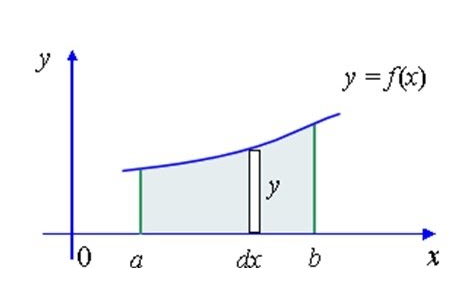
\includegraphics{fig_graphExample}
  \caption{integrating under a graph}
  \label{fig:preliminaryGraph}
\end{figure}

Let's say that $f$ is the 1 (or more) dimensional continuous function over $\R$ (or $\R^n$), and we are trying to find
the area under the graph. The first attempt at this might be the following (called Darboux sums): Given a partition the
domain $P = \{ x_1, x_2, ..., x_n\}$, we can make many rectangles which are all easy to measure. Then, as the partition
gets finner ($\operatorname{size}(P) \rw 0$, $|P| \rw \infty$), we will get a better an better approximation of the area. 

If we take this approach, we will introduce some level of choice: there are many ways in which this partition can be formed,
as well as a choice of the ``height'' of the rectangle. For example, you can choose the lowest or highest point:

\begin{figure}[H] 
  \centering
  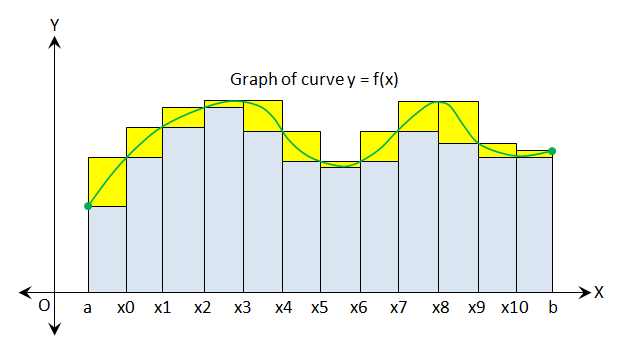
\includegraphics{fig_darbouxSumEx}
  \caption{lower and upper sums}
  \label{fig:darbouxSumEx}
\end{figure}

You can also choose any points in between, though what ``in between'' means starts to get hard to define in higher
dimensional spaces where different orders can be put onto the ``surfaces'' (or hyper-surfaces) of the top of the
rectangles (i.e.  hyper-rectangles). However, maximal and minimal point is always well defined on these surfaces (or
better, $\inf$ and $\sup$ always being well defined on these bounded surfaces), and even better, choosing the maximal
point for each rectangle height upper-bounds all possible other choices of Darboux sums, and the minimal point for each
rectangle's height lower-bounds all possible choices of Darboux sums. To be more precise, we'll replace the maximum and
minimum condition with $\sup$ and $\inf$, in which case the resulting sum is called the \emph{Riemann sum}.

Intuitively, the upper and lower Riemann sums must match up and exist as $\operatorname{size}(P) \rw 0$ and $|P| \rw
\infty$. It would be strange if they don't match up, and so we can (as a start) define a function that is not ``too
weird'' as one where the upper and lower Darboux sums match as $\operatorname{size}(P) \rw 0$, that is
\[
	\lim_{n \rw \infty}\sum_{i=1}^{n-1} \left(\inf_{[x_i, x_i+1]}f(x)\right) \cdot \left(x_{i+1} - x_i\right) = \lim_{n
	\rw \infty}\sum_{i=1}^{n-1} \left(\sup_{[x_i, x_i+1]}f(x)\right) \cdot \left(x_{i+1} - x_i\right)
\]
If this is the case, $f$ is said to be \emph{Riemann integrable}. Fortunately, it turns out that if $f$ is Riemann
integrable on one partition, it is Riemann integrable on all partitions, and so we don't need to ``remember'' our initial
choice of partition hen we say $f$ is Riemann integrable (we don't say ``$f$ is Riemann integrable on partition $p$, while
$f$ is not Riemann integrable on partition $q$''). 


All continuous functions over a bounded domains will be integrable (so trigonometric functions, polynomials, $\log$,
$\sqrt{\_\_}$ over the appropriate domain, and so forth). Since any geometric shape learnt in pre-university education
can be bounded by a continuous function, we have just generalized the idea of measuring those areas\footnote{though we
won't go into the details of finding those areas}. In fact, being continuous \emph{almost} encapsulates all possible
functions. To understand the generalization, consider 
\[
	f_{\text{no }1}: [-1,1] \rw \R, \qquad f_{\text{no }1}(x) \begin{cases}
						x^3 & x \ne 1\\
						0 & x = 1
					\end{cases}
\]
Notice that there is a gap in the line
\[
	\begin{tikzpicture}
	  \draw[->] (-3, 0) -- (4.2, 0) node[right] {$x$};
	  \draw[->] (0, -3) -- (0, 4.2) node[above] {$y$};
	  \draw[scale=0.5, domain=-3:3, smooth, variable=\x] plot ({\x}, {\x*\x});
	  \node[circle,draw, scale=0.1] (c) at (0,0){};
	\end{tikzpicture}
\]

however, this gap has ``zero measure'', we would think that the result should be the same. And in fact it is! The function
$f_{\text{no }1}$ is also Riemann integrable (as can be checked) and will have the same value as $x^3$ on $[-1,1]$. In
general, if finitely (or even countably) many points are ommited, then $f$ will still have the same measure. Since $f_{\text{no }1}$ is no
longer continuous, but it as just off by some finite number of points, we say that $f$ is continuous \emph{almost
everywhere} \footnote{Later, almost every continuous will mean continuous up to a zero measure set once we properly define
a measure}. It should be reviewed that $f$ is Riemann integrable if and only if $f$ is continuous almost everywhere. 

Stepping aside from measuring area under a graph for a moment, we turn to the study of another very common notion in
analysis: limits. Limits are of fundamental importance in Analysis. They are the tool used to construct or define many
different types of analytical objects (ex. $\R$, continuity, differentiability, Fourier series, sequences and series).
More generally, the concept (and formalisation) of a limit is how mathematicians get to study infinites which are
``well-defined''.
In my mind, limits are one of the distinguishing feature between algebra and analysis: many algebraic properties ``break
down''
or are different when we try to bring in more than finitely many objects (ex. products of infinite groups cannot be direct products in
\bf{Grp} since $1+1+\cdots$ is not defined (hence they are direct sums), the dimension of $\Q[x]$ and $\Q[[x]]$ as
$\Q$-algebras differ, etc.). A good definition of limit is important to be able to define objects ``at infinity'', since
if it is not well defined, then we can make the ``result'' non-unique. 

Here is a silly example of that: what is $\infty - \infty$? Maybe we can say that the answer is $0$? or $\infty$? If we are
not careful with our definition, it can actually be any number. First, ``notice'' that $1 + 1/2 + 1/3 + \cdots ``=''
\infty$, or more precisely, the series $S_{n} = \sum 1/n$ is unbounded from above. Since these two are ``equal'', we can
treat them as the same. Then assuming the usual algebraic
properties of distributivity work over countably many components, we hvae
\[
	(1 + 1/2 + 1/3 + \cdots) -  (1 + 1/2 + 1/3 + \cdots) = (1 + 1/2 + 1/3 + \cdots) - 1 - 1/2 - 1/3 - \cdots
\]
Now, pick any $ x \in \R$. Then this sequence can be ``rearranged'' to converge to that number. Start by picking $1$. If $x
> 1$, pick $1/2$, if it's less pick $-1$. Keep doing this, and this will evidentially converge to $x$! Thus $\infty
- \infty$ can be any real number we want!

This is why the idea of a limit is important: If the limit exists, we mean that there is a unique value for which the limit
will converge to. This is why limits are used to define objects with some ``countably infinite'' properties
\footnote{Object with some ``uncountably infinite'' or larger properties use a generalisation of a limit called an
\emph{ultra-filter} which we don't need to study in this course}. 

One important consequence of limits being unique is when we use limits to construct new functions from a limit of
functions! As review, you should check the construction of a \emph{continuous but nowhere differentiable function}. Another
example is with Fourier series and Fourier transformations which are used to encode and decode signals. Another example
the definition of compact exhaustion for imperfect integrals. There are many more yet to come as well!

Now, returning to integrals for a moment, we can ask ourselves if integrals commute with limits, that is
\[
	\lim_{n \rw \infty} \int f_n = \int \lim_{n \rw \infty} f_n
\]
where the limit here is \emph{pointwise limit}. Note that uniform limits (if it exist) will sort of commute:
\[
	\uniflim_{n \rw \infty} \int f_n = \int \lim_{n \rw \infty} f_n
\]

However, point-wise limit doesn't generally do

\begin{example}{Limit Doesn't Commute}{limitNoCommuteEx}
	Take $\chi_\Q: [0,1]\rw [0,1]$ to be the indicator function on $\Q$, that is
	\[
		\chi_\Q(x) = \begin{cases}
			1 & x \in \Q\cap [0,1]\\
			0 & \text{otherwise}
		\end{cases}
	\]
	Notice that $\chi_\Q$ is nowhere continuous, and hence is not Riemann integrable. We can see this more clearly by
	noticing that the upper Riemann sum is $1$ and lower Riemann sum is $0$. However
	\[
		g_n(x) = \begin{cases}
			1 & \text{if } \frac{p}{q},\ p,q \in \N, p \le n\\
			0 & \text{otherwise}
		\end{cases}
	\]
	is integrable, and $g_n \rw \chi_\Q$, that is $\lim_{n \rw \infty} g_n = \chi_\Q$. Notice that each $g_n$ are
	integrable, but $\chi_\Q$ is not, that is
	\[
		\lim_{n \rw \infty} \int g_n \ne \int \lim_{n \rw \infty} g_n
	\]
	Since the right hand side is not defined. 
\end{example}

Thus, our notion of integrability does not work will with limits! Thus, since integrals gives us useful ways of
analyzing our functions, and many functions are constructed as the limit of functions, we are going to spend lots of
time upgrading our notion of integrability to make it commute (under appropriate circumstances) with limits.To upgrade the notion of integration, there must be some
requirements we must keep in mind while finding a suitable replacement. In particular
\begin{enumerate}
	\item The area under the graph should be the same as the Riemann Integral
	\item Geometric intuition's should still be consistent, in particular
		\begin{enumerate}
			\item  if $f \le g$ then $\int f \le \int g$
			\item $\int af + bg = a\int f + b\int g$
		\end{enumerate}
	\item A set $A$ can be thought to be ``integrable'' if we define
		\[
			\chi_A(x) \begin{cases}
				1 & x \in A\\
				0 & x \notin A
			\end{cases}
		\]
		and $\int \chi_A$ is defined. 
\end{enumerate}

This last criterion is actually very interesting as it allows us to generalize the question from finding the area's
under graphs (or measuring the area under the graph) to figuring out how to measure sets in general! In fact, starting
by defining how to measure sets and then defining how to integrate function turns out to be a fruitful order in which we
can learn about this generalisation of integration. The reason this order is as actually an insight by Lebesgue:
defining the properties of something being ``measurable'' will allow us to re-define the integral with more rigour. Even
better, many different spaces can have different notions of a ``measure'' (for example, finite spaces where we measure
points, or probability spaces where sets represent the probability of an event, or physics where we might want to
measure the average density of a set), which the integral is the wrong concept (it's no longer strictly about ``area''),
but follows the same geometric intuitions as these other spaces (as we will show). Therefore, we will start by defining
the spaces over which we will want to define a way to measure sets. 

%Of course, we can try to redefine Riemann integration in terms of a measure too. This as done by Camille Jordan:

%\begin{defn}{Jordan Measure [Content]}{jordanMeasure}
	%Let $A \sse \R$. THen $A$ is said to be \emph{Jordan measurable} if $\int \chi_A$ exists. If that is the case, then
	%\[
		%m(A) := \int \chi_A
	%\]
%\end{defn}

%The definition puts in square bracekts the ord content since it will turn out that the Jordan measure fails to hold
%properties we will want measures to have. We will get back to this shortly 



\mainmatter
\chapter{Measures}

As a start, we might want to define a reasonable definition of what it means to measure any subset of $\R^n$. Such
a function would be of the form $\mu: P(\R^n) \rw [0, \infty]$. If $\mu$ were to exist, we would want our common
geometric intuitions to hold, that is:
\begin{enumerate}
	\item If $E_1, E_2, ..., E_n, ...$ is a countable collection of pair-wise disjoint subsets, then
		\[
			\mu \left(\bigcup_i E_i\right) = \sum_i \mu(E_i)
		\]
		\item If $E$ and $F$ are sets such that there is a function that only translates, rotates, and reflects $E$ to
			get to $F$ (i.e. a rigid motion), then $\mu(E) = \mu(F)$
		\item If $C$ is a unit cube in $\R^n$, then $\mu(C) = 1$
\end{enumerate}

However, these three axioms are inconsistent with one another! We have actually shown this by showing if $\mu$ is
defined on $P(\R^n)$ (even when $n = 1$), then we can construct \emph{Vitali sets} that will have to be both $0$ and
$\infty$ in measure -- a contradiction.

\begin{thm}{Vitali Sets Are Unmeasruable}{vitaliSetsAreUnmeasruable}
	Vitali sets are un-measurable
\end{thm}

\begin{Proof}
	Take $[0,1]$. Partition this set as follows:
	\[
		x\sim y \ \LRw\ x-y \in \Q
	\]
	In a sense, this is the set of cosets of $\R/\Q$ restricted to $[0,1]$; we will rely on this intuition to label the
	equivalence classes. Since $\R/\Q$ is the set of irrational numbers modulo rational numbers, let $N_q$ be an
	equivalence class of contains $x$ that is equivalent to the irrational number $q$. Notice that there are uncountably
	many such equivalence relations. 

	Now, pick one $p \in N_q$ for each equivalence class, and let $N$ be the collection of all these $p$'s, so $N$
	contains one point from each equivalence class (notice that the axiom of choice must be used to create a non-empty
	$N$). We'll show that $N$ is unmeasurable. 

	First, for each rational number $ r\in \Q\cap [0,1)$, define:
	\[
		N+r = \set{x+r}{x \in N\cap [0, 1-r)}\cup \set{x+r}{x \in N\cap (1-r,1)}
	\]
	Then clearly, $N+r \sse [0,1)$ for each $r \in \Q\cap [0,1)$, and furthermore, for each $x \in [0,1)$ there exists an $r$ such that $x \in N + r$.
	To show this, let's say $y \in N$ is the element that was picked from the equivalence class of of $[x]$. Then by our
	choice of $y$, $x \in N+r$ since $r = x-y$ if $x \ge y$, or $r = x-y+1$ if $x < y$. Next, notice that the $N+r$ also
	forms a partition: if $(N+r)\cap (N+s) \ne \emptyset$ then $x-r $(or $x-r+1$) would equal $x-s$ (or $x-s+1$), but
	they belond to distinct equivalence classes, and so $(N+r)\cap (N+s) = \emptyset$. 

	We have no reached the point where we can declare our contradiction. If $\mu$ satisfies the three wanted properties,
	by $(1)$ and $(2)$:
	\[
		\mu(N) = \mu(N\cap [0,1-r)) + \mu(N\cap (1-r, 1)) = \mu(N+r)
	\]
	for any $r \in \Q \cap [0,1)$. Since $\Q\cap [0,1)$ is countable and $[0,1)$ is the disjoint union of the $N+r$'s:
	\[
		1 = \mu([0,1)) = \sum_{r \in \Q\cap [0,1)}\mu(N+r)
	\]
	where $1 = \mu([0,1))$ comes from $(3)$. Now, we have two possibilities:
	\begin{enumerate}
		\item Either $\mu(N) = 0$, in which case each $\mu(N+r) = 0$ but then $0 = 1$ -- a contradiction
		\item Either $\mu(N) \ne 0$ (say $k$, so $\mu(N+r) = k$, but then $0 = \infty$ -- a contradiction
	\end{enumerate}
	In other words, no mater what $\mu(N)$ is, we will run into a contradiction!
\end{Proof}

As you can verify, this construction required that we take advantage of the countability condition (the 1st property).
You might ask if weakening it to only finitely many will fix the issue, but sort of crazily it does not! In 1924, Banach
and Tarski proved the following paradox now known as the \emph{Banach Tarski Paradox}: 

\begin{quote}
	Let $U$ and $V$ be open subsets of $\R^n$, $n \ge 3$. Then there exists a $k \in \N$ and subsets $E_1, E_2, ...,
	E_k$, $F_1, F_2, ..., F_k$ such that 
	\begin{enumerate}
		\item all $E_j$'s are disjoint and their union is $U$
		\item all $F_j$'s are disjoint and their union is $V$
		\item There exists a rigid motion from $E_j$ to $F_j$ for $j = 1, ..., k$
	\end{enumerate}
\end{quote}

This is kind of insane: this means that we can take a pea-size ball, and make into the size of the earth! This means
that the notion of ``geometry'' is not actually a consistent concept in general set theory! 

Fortunately for us, The sets $E_j$ and $F_j$ are very strange sets; most sets that are in fact measurable. To be more
precise, it is consistent to say that the axiom of choice fails and that all sets are Lebesgue measurable (which will be
the measure that will replace the Riemann integrability). For the purposes of this course, that means that any set
we construct without the axiom of choice (and just doing normal ZF  without any sneaky logical cheating) will be measurable.
For more details, see
\begin{center}
	\url{https://math.stackexchange.com/questions/1847052/most-functions-are-measurable}
\end{center}
	
\section{Sigma-Algebras and Properties}
Since the axiom of choice is the source of the problem of unmeasurability in the previous problems, we start by defining
a space on which we avoid unmeasurable sets, namely, we want to limit ourselves to \emph{countable} choices. The
definition should be pretty general, as it should accommodate measures in more general spaces. It should also be
``arithmetically expandable'', as in we should be able to measure smaller parts of the space (perhaps in more convenient
orientations) and add them all up. Thus, we define an \emph{algebra}:
\begin{defn}{Algebra and $\sigma$-Algebra}{algAndsigmaAlg}
	Let $X$ be an arbitrary set. Then let $\mathcal{A} \sse P(X)$ be a non-empty collection of subsets such that 
	\begin{enumerate}
		\item for any finite set of sets $A_1, A_2, ..., A_n \in \mathcal{A}$, $\bigcup_i A_i \in \mathcal{A}$
		\item For any $A \in \mathcal{A}$, $A^c \in \mathcal{A}$. 
	\end{enumerate}
	If it is closed under countable union, we call it a $\sigma$-algebra. We will usually denote $\sigma$-algebra on $X$
	as $\MM(X)$.
\end{defn}

The $\sigma$-algebra will be our natural space in which we will show in the next section we can define a ``measure
function'' without the previous contradiction. 

I like to think of the finite closure as a more general way of saying that a space is ``closed under
a function'', the function here being $\cup$. In this way, it's sort of the most general algebraic structure. Adding
the fact that it's closed under countable union brings us further way from the realm of algebra, and hence it's
a $\sigma$-algebra. The term sigma is very common to mean countable, for example, a space $\sigma$-compactness if it is
the countable union of compact subspaces. 

\begin{defn}{Measurable Space}{measurableSp}
	Let $X$ be a set and $\MM \sse P(X)$ be a $\sigma$-algebra. Then $(X, \MM)$ is called a \emph{measurable space} and
	a set in $\MM$ is called a \emph{measurable set}
\end{defn}


\begin{prop}{Properties of $\sigma$-algebra}{propSigmaAlg}
	Some immediate properties of a $\sigma$-algebra:
	\begin{enumerate}
		\item It is closed under countable intersection, since $\bigcap_i X_i = \left( \bigcup_i X \right)^c$, and by
			difference, since $X\setminus Y = X\cap Y^c$. 
		\item $\emptyset$ and $X \in \CA$, since for any $E \in \CA$, $E\cap E^c = \emptyset \in \CA$ and $E\cup E^c
			= X \in \CA$
		\item Any countable collection of subsets $\{E_i\}_{i=1}^\infty \sse \CA$ can be turned into a countable disjoint
			union, where
			\[
				F_k = E_k \setminus \left( \bigcup_{i=1}^{k-1}E_i\right) = E_k \cap \left(\bigcup_{i=1}^{k-1}E_i\right)^c
			\]
			and by what we've just shown, every $F_k \in \CA$, and by construction $\cup_i E_i = \cup_i F_i$. We will use
			this technique often very soon (note that not all sets are nonempty, that proof requires more set-theory
			manipulation).
		\item Given any family of $\sigma$-algebras on $X$, their intersection is also a $\sigma$-algebra. Because of this,
			given $Y \sse X$, there is always a unique smallest $\sigma$-algebra $\MM(Y)$ that contains $Y$ (there is at
			least always one, $P(Y)$, and so this concept is well-defined). $\MM(Y)$ is called the $\sigma$-algebra
			generated by $Y$. 
	\end{enumerate}
\end{prop}


A lemma we'll point out right now to simplify future proofs is the following:

\begin{lem}{}{sigmaAlgGeneratingSetContainement}

	If $Y \sse \MM(X)$, then $\MM(Y) \sse \MM(X)$
\end{lem}

\begin{Proof}
	Since $\MM(X)$ is a $\sigma$-algebra that contains $Y$, then it will contain all countable unions and compliment of
	$Y$, and hence it will contain $\MM(Y)$ (i.e. proposition~\ref{pr:propSigmaAlg}[4]). 
\end{Proof}

\begin{example}{$\sigma$-Algebras}{sigma-AlgebrasEx}
	\begin{enumerate}
		\item If $X$ is any set, then $\{\emptyset, X\}$ and $P(X)$ are trivially $\sigma$-algebras. Once we define
			measurable function, these will be the initial and final object in measurable spaces. 
		\item If $X$ is any set, then $P(X)$ is also a $\sigma$-algebra. Usually, we will use
			proposition~\ref{pr:propSigmaAlg}[5] and other tools to construct a smaller $\sigma$-algebra to not work with $P(X)$ since
			it's too big for most cases. 
		\item  If $X$ is an uncountable set, define
			\[
				\CA = \set{E \sse X}{\text{$E$ is countable or $E^c$ is countable}}
			\]
			this set is called the $\sigma$-algebra of countable and co-countable sets. It is useful when we want to make
			sure that the countable union of sets is still countable (or it's compliment is) \footnote{Sneakily, we use
			the axiom of choice for countably many choices to prove this is true}
	\end{enumerate}
\end{example} 

Another common $\sigma$-algebra generated on a set $X$ is related to a topology on $X$, that is, if $\TT(X)$ is
a topology, of $X$, we will define the following $\sigma$-algebra:
\begin{defn}{Borel $\sigma$-Algebra}{borelsigma-Algebra}
	Let $X$ be a set and $\TT(X)$ be a topology on $X$. Define the \emph{Borel $\sigma$-algebra} to be
	\[
		\BB_X := \MM(\set{U \sse X}{\text{$U$ is an open set contained in $X$}}
	\]
	The elements of $\BB_X$ are called \emph{Borel sets}
\end{defn}

The set $\BB_X$ will include the open sets, closed sets, countable union and intersection of closed sets, and the
countable union of countable intersections of open/closed sets, et cetera. 

Since the countable intersection of open sets and countable union of closed sets are not necessarily  open or closed sets
respectively\footnote{it is possible that the countable intersection/union of open/closed sets are open/closed, and so
the word ``necessarily'' is required}, but are members in $\BB_X$, we will give them names: A countable intersection of open sets is called
a $G_{\delta}$ set , and a countable union of closed sets is called a $F_\sigma$ set (F for \emph{ferm\'e}  in french,
$G$ because it's after $F$ in the alphabet). The $\sigma$ is for \emph{Summe} (sum in German) since it's a union
and the $\delta$ is for \emph{Durchschnitt} (intersection in German) since it's an intersection. We can continue this
pattern and define $G_{\delta \sigma}$ to be the countable union of countable intersection of open sets, $F_{\sigma
\delta}$ to be the countable intersection of countable union, and so and so on and so forth for any length of
interchanging $\sigma$'s and $\delta$'s. In general, this ``chain'' of unions and intersections does not need to
terminate, and a $F_{\sigma \delta}$ (as a simple example for a chain of length $2$, $\R\setminus \Q$ is
a $F_{\sigma\delta}$ set, but not a $F_\sigma$ set; use Baire's Categories theorem).
There will be cases in which it will terminate (in fact, the majority of measure's we'll work with will have this
terminate after at just $F_\sigma$ or $G_\delta$ ``up to a zero set'', see theorem~\ref{th:subsetOfRRepresentation}, and
example ref:HERE for a measure that does not terminate)

One of the most common Borel sets we will be working with is $\BB_\R$ with the usual euclidean topology on $\R$. It is
useful to have an of different generating sets for $\BB_\R$:

\begin{prop}{Generators For $\BB_X$}{generatorsForBorelSets}
	Let $\R$ be the real numbers and $\BB_\R$ be the Borel $\sigma$-aglebra on $\R$ given the standard euclidean
	topology $\TT(\R)$. Then the following generate $\BB_\R$:
	\begin{enumerate}
		\item The set of open intervals
		\item the set of closed intervals
		\item the set of half-open intervals
		\item the set of open rays
		\item the set of closed rays
	\end{enumerate}
\end{prop}

\begin{Proof}
	These proofs are quite easy to prove, and should be done as an exercise. A fact that you might need to recall is
	that every open set in $\R$ can be written as a countable union of open intervals (hint: $\R$ has a countable basis). 
\end{Proof}

\subsection*{Products and $\sigma$-Algebras}

Recall that the product between two sets is defined as $A\times B := \set{(a,b)}{a \in A, b \in B}$, or more generally
$\{X_\alpha\}_{\alpha \in A}$ for a collection of non-empty sets $X_\alpha$\footnote{If they were empty, then the
product would be empty}, with $X = \prod_{\alpha \in A} X_\alpha$,. As we
know from Category Theory, the product comes equipped with set functions $\pi_\alpha$ that satisfy the universal property of
products (or more generally, this is a limit over the discrete category). Though we have yet to give a category where
$\sigma$-algebras are the objects (we need to define what the morphisms are\footnote{this is done in chapter~\ref{cha:integration}}), we can already construct our set $\prod_\alpha X_\alpha$ that will
be the product of the $X_\alpha$ in the category of measurable spaces.

\begin{defn}{Product $\sigma$-Algebra}{prodSigAlg}
	Let $\{X_\alpha\}_{\alpha \in A}$ be a collection of non-empty sets and $X = \prod_{\alpha \in A} X_\alpha$. Let
	\[
		\bigotimes_{\alpha \in A} M_\alpha = \MM(\set{\pi_\alpha^{-1}(E_\alpha)}{E_\alpha \in M_\alpha,\ \alpha \in A})
	\]
	to be the \emph{product $\sigma$-Algebra} on $\{M_\alpha\}_{\alpha \in A}$, i.e., it is the $\sigma$-algebra
	generated by all of the pre-images of the sets in $M_\alpha$. 
\end{defn}

It is not difficult to check that the product $\sigma$-algebra is indeed a $\sigma$-algebra. If $|A|$ is countable we usually write $\bigotimes_{i=1}^\infty M_i$, and if $|A|$ is finite, we can write
$\bigotimes_{i=1}^n M_i$ or $M_1\bigotimes M_2 \bigotimes\cdots\bigotimes M_n$. Notice that since we allow for countable
unions, it is not so easy to represent $\bigotimes_{\alpha \in A} M_\alpha$ as the product of the elements of
$M_\alpha$, (just like for Groups in the category of \bf{Grp}), and hence why we do not use the $\prod$ or $\bigoplus$ notation.
On the other hand, the fact that only a countable union of elements is permitted will still limit the product in the number of non-trivial
components, hence justifying the $\bigotimes$ notation instead of $\prod$. In fact, it is the same as $\bigoplus$, but
instead of ``all but finitely many'', we have ``all but countably many'':
\begin{prop}{Countable Product $\sigma$-algebra}{countableSigAlg}
	Let $M_n = \MM(\CE_n)$ be a $\sigma$-algebra for $n \in \N$ where $\CE_n \sse P(X_n)$. If $X_n \in \CE_n$, then
	\[
		\bigotimes_{n=1}^\infty M_n = \MM\left(\set{\prod_{i=1}^n E_i}{E_i \in M_i}\right)
	\]
\end{prop}

\begin{Proof}
	The $\supseteq$ direction is easy (Take $\bigcap_{i=1}^n \pi_i(E_i)$ for appropriate values). For $\sse$, Since $X_i
	\in M_i$, we have that every element is inside the right hand side. Make sure you see why $X_n \in \CE_n$ makes
	a difference. By lemma~\ref{lm:sigmaAlgGeneratingSetContainement}, the result follows. 
\end{Proof}

We can further simplify our representation of $\bigotimes_{\alpha \in S} M_\alpha$ given a generating set for each
$M_\alpha$ (such a set always exists, namely $M_\alpha$ itself is always a generating set)

\begin{prop}{Generating set for Product $\sigma$-Algebra}{genSetSigAlg}
	Let $\{M_\alpha\}_{\alpha \in A}$ be a non-empty collection of $\sigma$-algebras, and let $\CE_\alpha \sse
	P(X_\alpha)$ be a generating set for $M_\alpha$. If $\FF = \cup_{\alpha \in A} \CE_\alpha$, then:
	\[
		\bigotimes_{\alpha \in A} M_\alpha = \MM(\set{\pi_\alpha^{-1} (E_\alpha)}{E_\alpha \in \CE_\alpha,\ \alpha \in
		A}) = \MM(\FF)
	\]
	Furthermore, if $|A|$ is countable and $X_\alpha \in \CE_\alpha$ for each $\alpha \in A$, then
	\[
		\bigotimes_{\alpha \in A} M_\alpha = \MM\left(\set{\prod_{\alpha \in A} E_\alpha}{E_\alpha \in \CE_\alpha,\
			\alpha \in A}\right)
	\]
\end{prop}

\begin{Proof}
	Dealing with the first case, the $\supseteq$ is clear since $E_\alpha \in \CE_\alpha$ implies $E_\alpha \in
	M_\alpha$, so $E_\alpha \in \bigotimes_{\alpha \in A}M_\alpha$. For the $\sse $ direction, If $E_\alpha \notin
	\CE_\alpha$, then since $\MM(\CE_\alpha) = M_\alpha$, some countable unions and intersections of elements of $\CE_\alpha$ equal
	$E_\alpha$, proving the $\sse$ direction. 

	The countable case follows proposition~\ref{pr:countableSigAlg}
\end{Proof}

\subsection*{Borel Spaces and Products}

A topological space of much study in Analysis is metric spaces. As a reminder, if $\{X_\alpha\}_{i=1}^n$ is
a collection of metric spaces, then $X = \prod_{i=1}^n X_i$ has the product metric which is the generalization of the
euclidean metric. As was seen in a topology class, the following metrics on a product space all define the same product
topology (for notational simplicity, let's work with two metric spaces $X$ and $Y$ and consider $X\times Y$):
\begin{enumerate}
	\item $d((x_1, x_2), (y_1, y_2)) = \max\{d_X(x_1, y_1), d_Y(x_2, y_2)\}$
	\item $d((x_1, x_2), (y_1, y_2)) = \sqrt{d_X(x_1, y_1)^2 + d_Y(x_2, y_2)^2}$
	\item $d((x_1, x_2), (y_1, y_2)) = d_X(x_1, y_1) + d_Y(x_2, y_2)$
\end{enumerate}

We can ask about establishing Borel sets $\BB_X$ on $X = \prod_{i=1}^n X_i$ with $X$ having the product measure. It is
tempting to say that this naturally splits into $\bigotimes \BB_{X_i}$, however, this is not always the case! This is
mainly due to the fact that not all topological spaces have a countable basis, and since we're allowing countable
intersection of open sets, this will actually create more sets than the if we take the product of the Borel spaces:
\begin{prop}{Borel sets on product Metric Space}{borelSetsandMetricSp}
	Let $X_1, ..., X_n$ be metric spaces, and $X = \prod_{i=1}^n X_i$ be the product metric space. Then
	\[
		\bigotimes_{i=1}^n \BB_{X_i} \sse \BB_X
	\]
	If the spaces $X_i$ are separable (i.e. has a countable dense subset, and since it's a metric space it means there
	is a countable basis), then
	\[
		\bigotimes_{i=1}^n \BB_{X_i} = \BB_X
	\]
\end{prop}

\begin{Proof}
	The proof of the $\sse$ direction rather simple. By proposition~\ref{pr:genSetSigAlg}, $\bigotimes_{i=1}^n
	\BB_{X_i}$ is generated by $\CE = \set{\pi_i^{-1}(U_j)}{U_j\text{ is open in $X_j$},\ 1 \le j \le n}$. Since the
	sets of $\CE$ are open in $X$, by lemma~\ref{lm:sigmaAlgGeneratingSetContainement}, $\bigotimes_{i=1}^n \BB_{X_i}
	\sse \BB_X$. 

	For the converse, since each $X_j$ is separable, each have a countable dense subset. Since $X_j$ is a metric space,
	we can form a countable basis with open balls with rational radii around each points in the countable dense subsets. 
\end{Proof}

As a consequence, $\bigotimes_{i=1}^n \BB_{\R} = \BB_{\R^n}$, since $\R$ has a countable dense subset. 

\subsection*{Elementary Sets}

This is a technical result needed for later (maybe introduce it as exercises?)

\begin{defn}{Elementary Family}{elementaryFamily}
	Let $X$ be a set and $\CE \sse P(X)$. Then $\CE$ is called an \emph{elementary family} if 
	\begin{enumerate}
		\item $\emptyset \in \CE$
		\item If $E,F \in \CE$ then $E\cap F \in \CE$
		\item If $E \in \CE$, then $E^c$ is a finite disjoint union of elements of $\CE$
	\end{enumerate}
\end{defn}

\begin{prop}{Elementary Families and Algebra}{ElementaryFamAndAlg}
	Let $\CE$ be an elementary family. Then the collection of finite disjoint unions of element of $\CE$ forms an
	algebra
\end{prop}

\begin{Proof}
	(TBD)
	Let $U, V \in \CE$, and consider $V^c = \dcup_{j=1}^J F_j$ (for disjoint $F_j \in \CE$). Then 
	\[
		U\setminus V = U\cap V^c = \dcup_{j=1}^J (U \cap F_j)
	\]
	notice that each $U\cap F_j \in \CE$. So
	\[
		U\cup V = (U\setminus V)\cup V = \dcup_{j=1}^J (U\cap F_j) \dcup V
	\]
	where $\dcup_{j=1}^J (U\cap F_j) \in A$

	Continuing inductively, 
\end{Proof}



(also, remember that separable means countable dense subset)
Once the course starts
\begin{enumerate}
	\item There is an interseting example ith logical statements!!
		\begin{figure}[H] 
		  \centering
		  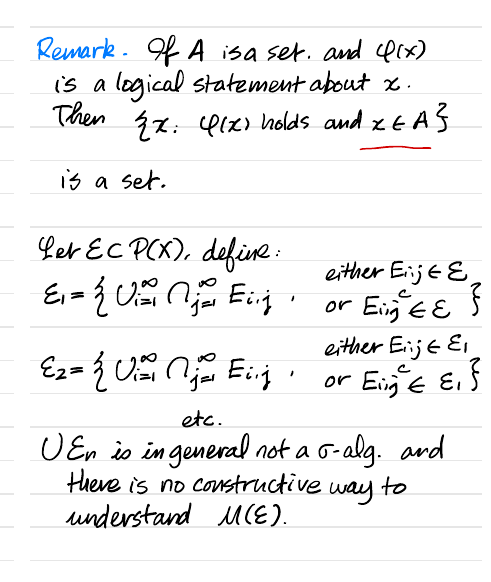
\includegraphics{fig_notSigmaAlgebraLogicEx}
		  \caption{fascinating!}
		\end{figure}
\end{enumerate}

\section{Measure}

We can finally define the function which will give us an idea of the ``size'' of sets:

\begin{defn}{Measure}{measure}
	Let $X$ be a set along with a $\sigma$-algebra $\MM$. A function $\mu: \MM \rw [0,\infty]$ is called
	a \emph{measure} on $\MM$ (or $(X, \MM)$ or even $X$ if the measure is clear from context) if
	\begin{enumerate}
		\item $\mu(\emptyset) = 0$
		\item \bf{(Countably Additivity)} If $\{E_i\}_{i=1}^\infty$ is a sequence of disjoint sets, then
			$\mu\left(\bigcup_{i=1}^\infty E_i\right) = \sum_{i=1}^\infty \mu(E_i)$ 
	\end{enumerate}

\end{defn}

Given that $(X, \MM)$ is a measurable space, along with a $\mu$ we can say the space has a measure:

\begin{defn}{Measure Space}{measureSp}
	Let $(X, \MM)$ be a measurable space. Then if $\mu$ is a measure on $X$, then $(X, \MM, \mu)$ is a \emph{measure
	space}
\end{defn}

If the 2nd condition of a measure was limited to a finite sequence (or more generally, all but countably many of the sets in the
sequence or nonempty), then we would say that it respects finite additivity. If $\mu$ respects finite but not countable
additivity, $\mu$ is called a \emph{finite additive measure}. 

Most measure's that we will work with have some finiteness condition associated with it:
\begin{defn}{Finiteness Condition on $\mu$}{finiteCondOnMu}
	Let $(X, \EM, \mu)$ be a measure space.
	\begin{enuemrate}
		\item If $\m(X) < \infty$, then $\mu$ is called a \emph{finite measure}
		\item if there exists sets $\{E_i\}_{i=1}^\infty \sse \EM$ such that $\bigcup_i^\infty E_i = X$ and $\mu(E_i)
			< \infty$ for all $E_i$, then $\mu$ is called a \emph{$\sigma$-finite measure}. More generally, if $E
			= \bigcup_{i=1}^\infty E_i$ for some sequence of $E_i$, then $E$ is called $\sigma$-finite on $\mu$ (some
			say that $E$ is said to be $\sigma$-finite on $\mu$)
		\item if for for all $E \in \EM$ such that $\mu(E) = \infty$, there exists a $D \sse E$, $D \in \EM$ such that $\mu(D) < \infty$, then $\mu$ is
			called a \emph{semi-finite measure}
	\end{enuemrate}
\end{defn}
If $\mu(X) < \infty,$ then this implies for all $S \in \MM$, $\mu(S) < \infty$ (as can quickly be checked). Naturally,
all finite measure's are $\sigma$-finite, and all $\sigma$-finite measure are semi-finite, but the converses are not
true (as we'll explore in the following examples). Note too that most measure's we will be working over will be
$\sigma$-finite (think of $\R$ with the intuitive notion of length of an interval). 


\begin{example}{Measures}{meauresEx}
	\begin{enumerate}
		\item Let $X$ be nonempty, $\MM = P(X)$, and $f: X \rw [0,\infty]$. Then we can define 
			\[
				\mu_f(E) = \sum_{e \in E} f(e)
			\]
			where the sum can be infinite (the domain of $f$ is the positive part of the extended real numbers). Notice
			that $f$ is semifinite if and only if $f(x) < \infty$ for all $x \in X$, and $\mu$ is $\sigma$-finite if and
			only if $\mu$ is semi-finite and $\set{x}{f(x) > 0}$ if countable. 

			If $f(x) = 1$ for all $x \in X$, then $\mu_f$ is called the \emph{counting measure}. On the other hand, if
			for some $x_0 \in X$, $f(x_0) = 1$ and $f(x) = 0$ if $x \ne x_0$, then $\mu_f$ is called a \emph{point mass}
			or \emph{Dirac measure} at $x_0$
		\item Let $X$ be an uncountable set an $\MM$ be the $\sigma$-algebra of countable or co-countable sets (recall
			example~\ref{ex:sigma-AlgebrasEx}). Define
			\[
				\mu(E) = \begin{cases}
					0 & \text{$E$ is countable}\\
					1 & \text{$E$ is co-countable}
				\end{cases}
			\]
			Then $\mu$ is a measure!
		\item An example of an finite additive measure that is not a measure is the following: let $X$ be some infinite
			set and $\MM = P(X)$. Define $\mu$ to be
			\[
				\mu(E) = \begin{cases}
						0 & \text{$E$ is finite}\\
						\infty & \text{$E$ is infinite}
					\end{cases}
				\]
				Then $\mu$ is an finite additive measure, but not a measure
	\end{enumerate}
\end{example}


\begin{prop}{Properties of Measures}{propMeasure}
	Let $(X, \MM, \mu)$ be a measure space. Then
	\begin{enumerate}
		\item \bf{(Monotonicity)} Let $E, F \in \MM$ and $E \sse F$. Then $\mu(E) \le \mu(F)$
		\item \bf{(Subadditivity)} if $\{E_i\}_{i=1}^\infty \sse \MM$, then $\mu\left(\cup_i\mu(E_i)\right) \le \sum_i \mu(E_i)$
		\item \bf{(Continuity from Below)} if $\{E_i\}_{i=1}^\infty \sse \MM$, and $E_1 \sse E_2 \sse \cdots$, then
			\[
			\mu \left(\cup_i E_i\right) = \lim_{i \rw \infty} \mu(E_i)
		\]
	\item \bf{Continuity from Above} if $\{E_i\}_{i=1}^\infty \sse \MM$ and $E_1 \supseteq E_2 \supseteq$
		\emph{and} $\mu(E_1) < \infty$. Then
			\[
				\mu \left(\cap_i E_i\right) = \lim_{i \rw \infty} \mu(E_i)
		\]
	\end{enumerate}
\end{prop}

\begin{Proof}
	here. Do them as exercises!
\end{Proof}

Notice that for (d), we can instead limit it to $\mu(E_i) < \infty$ for some $i$, and the proof remains the same. We
still require that some $i$ exists such that $\mu(E_i) < \infty$, for it's possible that all $\mu(E_i)$ is infinite, but
$\mu(\cap_i E_i) < 0$. For example, take the measurable space $(\N, P(\N))$ with the counting measure. Then the sets
\[
	E_i = \set{n \in \N}{ n \ge i}
\]
then every $E_i$ is infinite but their intersection is empty and thus has measure $0$ in the counting measure. 

\subsection*{zero measure sets}

Frequently, there are sets in our measure that have a ``trivial size'' in the current measure. This is akin to when we
integrate, the border has no effect on the value of the integral. Such sets are said to be zero sets or null set:
\begin{defn}{Null Set}{nullSet}
	Let $(X, \MM, \mu)$ be a measure space and $E \in \MM$. Then if $\mu(E) = 0$, $E$ is said to be a \emph{null set} or
	\emph{zero set}. 
\end{defn}

By countably subadditivity, the countable union of null sets is a null set, hence null sets are ``invariant'' under
countable union. Due to this, we can work with measurable sets in $\MM$ \emph{up to null sets}. We shall often state in
proofs that a statement is true \emph{almost everywhere} (often abbreviated to a.e.) if it is true on the sets except
for the null sets. 

If we take $E \in \MM$ such that $\mu(E) = 0$, then by monotonicity, if $F \sse E$ the $\mu(F) = 0$, \emph{provided that
$F \in \MM$}. This is not always the case:

\begin{example}{Not Complete Space}{notComplSp}
	Partition $[0,1]$ into 10 (really any number) of subintervals, $\left[ \frac{i}{n}, \frac{i+1}{n}\right]$ for $0 \le
	i \le 9$, and let each of their measures be $0$. Take $\EM$ to be the $\sigma$-algebra defined on this set. Then
	is clearly an uncountable number of sets that do not have a measure defined on them that are subset of zero-measure
	sets.
\end{example}

However, adding all of these $F$'s that are subsets of null sets does not break our measure. A measure who's domain
includes all subsets of null sets is a \emph{complete measure} (i.e. the $\sigma$-algebra is closed under subsets of
null sets). Proving that this is still a measure is useful to eliminate future ``trivial obstructions'' to our proofs:

\begin{thm}{Completing a Measure}{measureCompleting}
	Let $(X, \MM, \mu)$ be a measure space. Let $\EN = \set{N \in \MM}{\mu(N) = 0}$ and $\oln{\MM} = \set{E\cup F}{E \in
	\MM\text{ and } F \sse N\text{ for some $N \in \EN$}}$. Then $\oln{\MM}$ is also a $\sigma$-algebra, and there is
	a \emph{unique} extension $\oln{\mu}$ of $\mu$ that is a complete measure on $\oln{\MM}$ that restricts to the
	measure of $\mu$ on $\MM$
\end{thm}

\begin{Proof}
	First of all, since $\MM$ and $\EN$ are both closed under countable union, so $\oln{\MM}$ is closed under countable
	union. To show it's closed under compliments, consider some $E\cup F \in \oln\EM$ ($E \in \EM$, $F \sse N \in \EN$).
	Without loss of generality, assume $E\cap N = \emptyset$ (if not, take $F\setminus E$ and $N\setminus E$ and
	continue the proof, then this will have he same value as our original $E\cap N$). Then 
	\[
		E\cup F = (E\cup N) \cap (N^c \cup F)
	\]
	So we get
	\[
		(E\cup F)^c = (E\cup N)^c\cup (N\setminus F)
	\]
	Since $E\cup N \in \EM$, $(E\cup N)^c \in \EM$. Since $N \setminus F \in \EN$, Since it's closed under union,
	$(E\cup F)^c \in \oln\EM$. Thus $\oln\EM$ is a $\sigma$-algebra. 

	Since $\oln\EM$ is a $\sigma$-algebra, we can try to define a measure, and indeed
	\[
		\oln\mu(E\cup F) = \mu(E)
	\]
	is a well-defined measure. If 
	\[
		E_1 \cup F_1 = E_2 \cup F_2
	\]
	Then $E_1 \sse E_2 \cup F_2$, and so by monotonicity:
	\[
		\mu (E_1) \le \mu (E_2 \cup F_2) \le(E_2 \cup N_2) = \mu(E_2) + \mu(N_2) = \mu(E_2)
	\]
	Similarly, $\mu(E_1) \ge \mu(E_2)$. Thus $\oln\mu (E_1\cup F_1) = \oln\mu(E_2\cup F_2)$, and so $\oln\mu$ is
	well-defined. Since $\oln\mu$ has all subsets of zero-sets in its domain, it is a complete measure. 

	Furthermore, if $\oln\nu$ was another complete measure on $\EM$, then it is easy to see that $\oln\nu = \oln\mu$,
	(since if it were different, then some subset of a zero-set must have non-zero measure, a contradiction to
	monotonicity) showing that $\oln\mu$ is unique. 
\end{Proof}

\begin{defn}{Completion of Measure}{measureCompletion}
	Let $(X, \MM, \mu)$ be a measurable space. Then $\oln{\MM}$ and $\oln{\mu}$ is called the \emph{completion of $\MM$
	with respect to $\mu$} and the \emph{completion of $\mu$} respectively
\end{defn}

\section{Outer Measure}

We now move on to constructing a particular type of measure which is draws inspiration from how we measured area's when
we calculated Riemann Integrals. In the abstract, when we tried defining a Jordan measure (or content\footnote{since
``Jordan measures'' only allow finite additivity, some don't like to use the word measure and opt for the word
content. In this book, we would say \emph{finite additive measure} as has already been stated earlier}), we
approximated the inner area of a shape $E$ in $\R^n$ by the limit of sums of rectangles contained in $E$, and the outer-area of $E$ in
$\R^n$ by the limit of the sums of rectangles containing $E$. The two numbers are called the inner and outer area of
$E$. If the two matched, we would call the result the area of $E$. This intuition can be generalized to the countable
case, except we can replace rectangles with some other ``basic sets'' that we might want that form an algebra.
Furthermore, the intuition of having the ``inner area'' and ``outer-area' is actually a bit restricting to work with in
the general measure case, and so that condition will be replaced with a different measureability condition we will soon
introduce. 

For the sake of generality, we will start by definition a more general notion of the measure called the outer-measure,
and then build-up on how form the outer-measure, we can get a measure that satisfies this generalization of Riemann
integration:

\begin{defn}{Outer Measure}{outerMeas}
	A function $\mu^*: P(X) \rw [0,\infty]$ is called an \emph{outer measure} if
	\begin{enumerate}
		\item $\mu^*(0) = \emptyset$
		\item if $A \sse B$, then $\mu^*(A) \le \mu^*(B)$
		\item $\mu^*\left(\bigcup_{i=1}^\infty A_i\right) \le \sum_{i=1}^\infty \mu^*(A_i)$ (even if the sets are
			disjoint!)\footnote{We will return to see when equality holds in definition~\ref{df:muStarMeasurable}}
	\end{enumerate}
\end{defn}

Note that we have not yet proven that an outer-measure is a measure; in particular notice that the domain is the
powerset. What we will do is define a generalization of the Riemann integral that will be our ``base-line'' for the
outer-measure:
\begin{prop}{Outer Measure Construction}{outMeasConstr}
	Let $\CE \sse P(X)$ where $\emptyset, X \in \CE$, and let $\rho: \CE \rw [0,1]$ where $\rho(\emptyset) = 0$. For any
	$A \sse X$, define
	\[
		\mu^*(A) = \inf\set{\sum_{1}^\infty \rho(E_j)}{E_j \in \CE\text{ and } A \sse \bigcup_{1}^\infty E_j}
	\]
	Then $\mu^*$ is an outer measure
\end{prop}

\begin{Proof}
	First, this measure is well-defined since for any $A \sse X$, If we take $E_i = X$, then $A \sse \cup_i E_i$. Next,
	we verify the 3 properties
	\begin{enumerate}
		\item Clearly, $\mu^*(\emptyset) = 0$ by taking $E_i = \emptyset$ for all $i$
		\item If $A \sse B$, then let $\CA$ and $\CB$ sets that correspond to $\mu^*(A)$ and $\mu^*(B)$. Then since all
			of the elements of $\CA \supseteq \CB$, by the property of the infimum $\inf \CA \le \inf \CB$, which
			transferring notations gives us $\mu^*(A) \le \mu^*(B)$
		\item Let $\{E_i\}_{i=1}^\infty \sse P(X)$ be a collection of (not necessarily disjoint) subsets. Let $\epsilon
			> 0$. Consider $\mu^*(E_k)$ for some $E_k \in \{E_i\}_{i=1}^\infty$. By the property of the infimum, there
			must exist some $\{F_j^k\}_{j=1}^\infty$ such that $E_i \sse \cup_j F_j^k$ where $\sum_{j=1}^\infty
			\rho(F_j^k) \le \mu^*(E_k) + \epsilon 2^{-k}$. 

			Now, let $E = \cup_i E_i$. By construction, $E \sse \cup_{i,k = 1}^\infty F_j^k$, and 
			\[
				\sum_{j,k} \rho(F_j^k) \le \mu^*(A) + \epsilon
			\]
			Since $\epsilon$ can be arbitrarily small, this completes the proof. 
	\end{enumerate}
\end{Proof}

As mentioned before, an outer-measure is not necessarily a measure. What we will do to allow this to be a measure is
single out sets that have the following property

\begin{defn}{$\mu^*$-measureable}{muStarMeasurable}
	Let $E \sse X$ be a set and $\mu^*$ be an outer measure on $X$. Then $E$ is called \emph{$\mu^*$-measurable} if 
	\[
		\mu^*(S) = \mu^*(S\cap E) + \mu^*(S\cap E^c) \quad \forall S \sse X
	\]
	In other word, if $E$ can naturally ``split'' a set $S$ into a part that's ``inside'' $E$ or ``outside'' $E$. The
	set $S \sse X$ is called the \emph{test set}. 
\end{defn}

By definition of the outer measure, since $S = (S\cap E)\cup(S\cap E^c)$:
\[
	\mu^*(S) \le \mu^*(S\cap E) + \mu^*(S\cap E^c) \quad \forall S\sse X
\]
Therefore, what is more important is to check the $\ge$ direction. Furthermore, if $\mu^*(A) = \infty$. Then $\ge$ holds
trivially, so to show a set is $\mu^*$ measurable, it is equivalent to show that for all finite measure sets $A$,
$\mu^*(S) \ge \mu(S\cap E) + \mu(S\cap E^c)$. 

As mentioned in the definition, this gives us a sense of being able to measure the ``inside'' and ``outside'' of a set.
If $E \sse A$, that is the $\mu^*$-measurable set belong in a better set, then $\mu^*(S) = \mu^*(S\cap E)
+ \mu^*(S\setminus E)$ which can be thought of as saying that we are measuring $S$ from the ``inside'' of $E$ and the
``outisde'' of $E$, and getting the same result. In fact, if $\mu^*(X) < \infty$, then we can define $\mu_*(E) = \mu^*(X)
- \mu(E^c)$, and have that $E$ is $\mu^*$-measurable if and only if $\mu_*(E) = \mu^*(E)$ aligning with our intuition
for inside equalling outside (see exercise ref:HERE). We do not do this method since it requires some finiteness condition on $\mu$. We can
conversely define $\mu_*$ in terms of supremums and need that $E$ contains the collection of $\cup_i A_i$, and that the
elements of $\{A_i\}_{i=1}^\infty$ must be disjoint (see exercise ref:HERE).

The big thing that is in the way of saying that an outer measure is a measure is that its domain is $P(X)$, which can
cause problems when $X$ is uncountable. However, all sets that satisfy  $\mu^*$-measureability turn out form
a $\sigma$-algebra and make $\mu^*$ a complete measure!

\begin{thm}{Carath\'eodory's Theorem}{carathThm}
	Let $\mu^*$ be an outer measure on $X$, and let $\MM$ be the collection of $\mu^*$-measurable sets. Then $\MM$ forms
	a $\sigma$-algebra, and the restriction of $\mu^*$ to $\MM$ is a complete measure 
\end{thm}

Notice that in the process of defining this measure, we started with the powerset, and then simply choose all sets that
restrict (which we will show forms a $\sigma$-algebra). In this way proving a function is an outer-measure is a little
less finicky since we don't need to be so careful in defining over which $\sigma$-algebra we want to define it over: the
$\sigma$-algebra comes with $\mu^*$

\begin{Proof}
	Let $\MM$ be the collection of $\mu^*$-measurable sets. Clearly, $\emptyset \in \MM$ since for all $S \sse X$:
	\[
		 \mu^*(S\cap \emptyset) + \mu^*(S\cap X) = 0 + \mu^*(S)
	 \]
	 implying $\mu^*$-measureability. Next, $\MM$ is closed under compliments, since if $E \in \MM$, then
	 \[
		 \mu^*(S) = \mu^*(S\cap E) + \mu^*(S\cap E^c) = \mu^*(S\cap E^c) + \mu^*(S\cap E)
	 \]
	 which also shows that $X \in \MM$. Finally, we need to show that $\MM$ is closed under countable unions. We'll
	 start by showing finite unions, which then means it suffices to show the union of two sets is closed (due to
	 induction). Let $A,B \in \MM$. As we remarked, it suffices to show that for any $E \sse X$ such that  $\mu^*(E)
	 < \infty$ that $\mu^*(E) \ge \mu^*(E\cap (A\cup B)) + \mu^*(E\cap(A\cup B)^c)$. Since $A$ and $B$ are $\mu^*$ measurable, we have
	 \begin{align*}
		 \mu^*(E) &= \mu^*(E\cap A) + \mu^*(E\cap A^c) & \text{$E$ is the test set}\\
				  &= \mu^*(E\cap A\cap B) + \mu^*(E\cap A\cap B^c)\\
				  &\quad + \mu^*(E\cap A^c\cap B) + \mu^*(E\cap A^c\cap B^c) & \text{$E\cap A$ and $E\cap A^c$ are the
				  test sets}
	 \end{align*}
	 Then notice we can write
	 \[
		 A\cup B = (A\cap B) \cup (A\cap B^c) \cup (A^c\cap B)
	 \]
	 Thus, using subadditivity, we can re-write 3 of the terms in the previous expression as:
	 \[
		  \mu^*(E\cap A\cap B) + \mu^*(E\cap A\cap B^c) +\mu^*(E\cap A^c\cap B)\ge \mu^*(E\cap A\cup B)
	 \]
	 Since $E\cap A^c\cap B^c = E\cap(A\cup B)^c$, we get:
	 \[
		 \mu^*(E) \ge \mu^*(E\cap (A\cup B)) + \mu^*(E\cap(A\cup B)^c)
	 \]
	 showing that $\MM$ is closed under finite union. Since $\MM$ is closed under compliment and contains $\emptyset$,
	 $\MM$ is an algebra. Even better, If we let $A$ and $B$ be disjoint, and let $A\cup B$ be the test set, then since
	 $A$ is $\mu^*$ measurable:
	 \[
		 \mu^*(A\cup B) = \mu^*((A\cup B)\cap A) + \mu^*((A\cup B)\cap A^c) = \mu^*(A) + \mu^*(B)
	 \]
	 showing that $\left.\mu^*\right|_\MM$ is a finitely additive measure. 

	 Next, we must show that $\MM$ is a $\sigma$-algebra, which as a consequence will show that $\left.\mu^*\right|_\MM$
	 is a measure. Let $\{E_i\}_{i=1}^\infty \sse \MM$. To simplify our task, re-construct $\{E_i\}_{i=1}^\infty$ to
	 be the set of disjoint sets $\{D_i\}_{i=1}^\infty$. Let $B_n = \bigcup_{i=1}^n D_i$ and $B
	 = \bigcup_{i=1}^\infty D_i$. Our goal is to show that for any $E \sse X$ such that $\mu^*(E) < \infty$ that
	 $\mu^*(E) \ge \mu^*(E\cap B) + \mu^*(E\cap B^c)$. We will start by considering $\mu^*(E\cap B_n)$:
	 \begin{align*}
		 \mu^*(E\cap B_n) &=  \mu^*(E\cap B_n\cap D_n) + \mu^*(E\cap B_n\cap D_n^c) & \text{$E\cap B_n$ is the test
		 set}\\
						  &= \mu^*(E\cap D_n) + \mu^*(E\cap B_{n-1})
	 \end{align*}
	 Notice that on the right hand side we have diminished to the case of $E\cap B_{n-1}$ from $E\cap B_n$. Using
	 induction, we can see that the expression simplifies to
	 \[
		 \mu^*(E\cap B_n) = \sum_{i=1}^n \mu^*(E\cap D_i)
	 \]
	 Continuing, since $B_n$ is measurable
	 \[
		 \mu^*(E)  = \mu^*(E\cap B_n) + \mu^*(E\cap B_n^c) \overset{!}{\ge} \mu^*(E\cap B_n) + \mu^*(E\cap B^c)
		 = \sum_{i=1}^n \mu^*(E\cap D_i) + \mu^*(E\cap B_n^c)
	 \]
	 where $\overset{!}{\ge}$ comes from monotonicity after switching $B_n^c$ to $B^c$. Since this equality holds true
	 for all $n$, we get:
	 \begin{align*}
		 \mu^*(E) &\ge \sum_{i=1}^\infty \mu^*(E\cap D_i) + \mu^*(E\cap B^c)\\
				  &\ge \mu^*\left(\bigcup_i E\cap D_i\right) +\mu^*(E\cap B^c)& \text{subadditivity}\\
				  &= \mu^*(E\cap B) +\mu^*(E\cap B^c) &\text{by construction of $E\cap B$}\\
				  &\ge \mu^*(E) & \text{subadditivity}
	 \end{align*}
	 Since we got $\mu^*(E) \ge \mu^*(E)$, we see that in fact all inequalities are equalities, getting us that
	 \[
		 \mu^*(E) = \mu^*(E\cap B) + \mu^*(E\cap B^c)
	 \]
	 showing us that $B \in \MM$. Furthermore, replacing $E = B$ in the previous proof shows us that
	 \[
		 \mu^*(B) = \sum_{i=1}^\infty \mu^*(D_i)
	 \]
	 giving us that $\mu^*$ is a measure on $\MM$. 

	 Finally, we must show that $\MM$ is complete, that is, if $E \in \MM$ such that $\mu^*(E) = 0$, then all subsets of
	 $E$ are in $\MM$. Notice that since $\mu^*$ is defiend on all of $P(X)$, it is equivalent to show that if $\mu^*(A)
	 = 0$, then $A \in \MM$. Then for any test set $E$, by monotonicity:
	 \[
		 \mu^*(E) \le \mu^*(E\cap A) + \mu^*(E\cap A^c) = 0 + \mu^*(E\cap A^c) \le \mu^*(E)
	 \]
	 meaning equality holds, showing that $A \in \MM$. Thus, $\left. \mu^*\right|_{\MM}$ is a complete measure, as we
	 sought to show. 
\end{Proof}

Carath\'eodory's Theorem is quite useful being able to state the existence of a measure given an outer-measure, but it's
not good to construct a measure (for example, can you tell me a non-trivial element in $\MM$ without directly appealing
to the definition?). The following concept is used to more systematically construct the set $\MM$ and the measure $\mu$
induced by $\mu^*$:

\begin{defn}{Premeasure}{preMeas}
	Let $(X, \CA)$ be an algebra. Then $\mu_0$ is called a \emph{premeasure} if
	\begin{enumerate}
		\item $\mu_0(\emptyset) = 0$
		\item \bf{``Respects'' countable union}: If $\{A_i\}_{i=1}^\infty \sse \CA$ is a collection of disjoint such
			that $\cup_i A_i \in \CA$, then $\mu_0(\cup_i A_i) = \sum_i \mu_0(A_i)$
	\end{enumerate}
\end{defn}

Note that the premeasure is automatically finitely additive since we can let all but finitely many of the terms in $(2)$
be $\emptyset$ (and hence are a stronger condition than finitely additive measure). However, it is not yet a measure
since it's domain is not necessarily closed under countable union. However, if it is closed for countable union for
a particular collection, that collection must satisfy the ``countable'' condition. Interestingly, by the definition of
an algebra, this implies that the countable union can be represented as a finite union and intersection of elements from
$\CA$. 

As before, we can define semifinite and $\sigma$-finite in a similar way. Using $\mu_0$, we can define the following
outer-measure:
\[
	\mu^*: P(X) \rw [0, \infty]\quad \mu^*(E) = \inf \set{\sum_i^\infty\mu_0(A_i)}{A_i \in \CA,\ E \sse \cup_i A_i}
\]

\begin{prop}{Premeasure To Measure}{preMeasToMeas}
	Let $\mu_0$ be a premeasure on $\CA$, and let $\mu^*$ be defined as above. Then
	\begin{enumerate}
		\item $\left.\mu^*\right|_{\CA} = \mu_0$
			\item Every set in $\CA$ is $\mu^*$-measurable
	\end{enumerate}
\end{prop}

Essentially, $\mu^*$ is an extension of $\mu_0$ and the associated restriction of $\mu^*$ to a measure will contain
$\CA$

\begin{Proof}
	\begin{enumerate}
		\item Let's show $\le$ and $\ge$ for any $E \in \CA$. The $\le$ direction is obvious since $\mu^*(E) \le
			\mu_0(E)$ since $E \sse \bigcup_{i=1}^\infty A_i$ where $A_1 = E$ and $A_i = \emptyset$ for $i > 1$, and so
			it is part of the set over which we take the infimum, and so the result \emph{has} to be smaller. 

			For the $\ge$ direction, let's say $E \sse \bigcup_{i=1}^\infty A_i$ for any $\{A_i\}_{i=1}^\infty \in \CA$.
			Let $B_n = E\cap \left(A_n \setminus \cup_1^{n-1}A_i\right)$. Then the collection $\{B_i\}_{i=1}^\infty$ is
			a disjoint collection of members of $\CA$ whose union is $E$. Thus, by the property of premeasure
			\[
				\mu_0(E) = \sum_1^\infty \mu_0(B_i) \overset{!}{\le} \sum_1^\infty \mu_0(A_i)
			\]
			where the $\overset{!}{\le}$ inequality comes from the fact that $\mu_0(B_i) \le \mu_0(A_i)$. Since this is
			true for any arbitrary collection $\{A_i\}_{i=1}^\infty$, it follows that 
			\[
				\mu_0(E) \le \mu^*(E)
			\]
			Thus establishing equality
		\item We need to show that for any $E \sse X$ and $A \in \CA$, $\mu^*(E) = \mu^*(E\cap A) + \mu^*(E\cap A^c)$.
			As mentioned earlier, it suffice to prove $\ge$ where $\mu^*(E) < \infty$. 

			Let $\epsilon > 0$. By the property of the infimum, there exists a subset $\{B_i\}_{i=1}^\infty \sse \CA$
			where $E\sse \cup_i B_i$ such that $\sum_i^\infty \mu_0(B_i) \le \mu^*(E) + \epsilon$. By part (1), $\mu^*$ is
			[countably] additive on $\CA$ (since it equals the pre-measure)
			\begin{align*}
				\mu^*(E) + \epsilon &\ge \sum_{i=1}^\infty \mu_0(B_i\cap A) + \sum_{i=1}^\infty (B_i\cap
				A^c)&\text{additivity}\\
					&\ge \mu^*(E\cap A) + \mu^*(E\cap A^c) &\text{monotinicity}
			\end{align*}
			and since $\epsilon$ was arbitrary, $A$ must be $\mu^*$-measurable, completing the proof
	\end{enumerate}
\end{Proof}

We can in fact be more precise with the measures that extend a premeasure: 

\begin{thm}{Premeasure Extensions}{preMeasExt}
	Let $\CA \sse P(X)$ be an algebra, $\mu_0$ a premeasure on $\CA$, and $\MM = \MM(\CA)$ (i.e. $\MM$ is the
	$\sigma$-algebra generated by $\CA$). Let $\mu$ be the extension of $\mu_0$ from proposition~\ref{pr:preMeasToMeas}.
	Then if $\nu$ is another measure on $\MM$ that extends $\mu_0$, then
	\[
		\nu(E) \le \mu(E)\qquad \forall E \in \MM
	\]
	with equality when $\mu(E) < \infty$ (i.e., it possible that $\mu$ is infinite while $\nu$ is finite). 

	If $\mu_0$ is $\sigma$-finite, then $\mu$ is the unique extension of $\mu_0$ to a measure on $\MM$
\end{thm}

In other words, we can extend a pre-measure to a measure by knowing what it does on the algebra (which in most cases
will be a collection of simpler sets, like intervals or rectangles), and then what happens on the rest of the measurable
sets we use the infimum definition. If we define another extension of $\mu_0$, then that measure will be \emph{finer}
than the $\mu$ given by $\mu^*$, i.e, $\mu$ is the \emph{coarsest} extension. If $\mu_0$ is $\sigma$-finite, then this
will in fact be the only extension of $\mu_0$

\begin{Proof}
	Let's say $\nu$ is an extension of $\mu_0$ so that $(X, \MM(\CA), \nu)$ is a measure space. To show that $\nu(E) \le
	\mu(E)$, let's say $\{A_i\}_{i=1}^\infty \sse \CA$ where $E \sse \cup_i A_i$. Then since $\nu$ is a measure, it is
	sub-additive on non-disjoint sets, and so
	\[
		\nu(E) \le \sum_i\nu(A_i)
	\]
	Since $\nu$ extends $\mu_0$, by proposition~\ref{pr:preMeasToMeas} $\left.\nu\right|_{\CA} = \mu_0$, so
	\[
		\nu(E) \le \sum_i\nu(A_i) = \sum_i\mu_0(A_i)
	\]
	Since  $\{A_i\}_{i=1}^\infty$ was an arbitrary choice, this works for any collection, and so
	\[
		\nu(E) \le \mu(E)\ \ [=\mu^*(E)]
	\]

	We show that $\nu(E) = \mu(E)$ if $\mu(E) < \infty$. Let $A = \cup_i A_i$ for some collection $\{A_i\}_{i=1}^\infty
	\sse \CA$. Then
	\[
		\nu(A) = \lim_{n \rw \infty} \nu\left(\bigcup_{i=1}^n (A_i)\right) = \lim_{n \rw \infty}
		\mu\left(\bigcup_{i=1}^n (A_i)\right)= \mu(A)
	\]

\end{Proof}

If $\mu$ is not $\sigma$-finite, then there can be more than one extension:

\begin{example}{2 extensions of pre-measure}{2ExtOfPreMeas}
			\begin{enumerate}
				\item Let $\CA$ be the collection of finite unions of the sets of the form $(a,b]\cap \Q$ with $-\infty
					\le a\le b\le \infty$. Then $\CA$ is an algebra on $\Q$ 
		\begin{Proof}
			Recall proposition \ref{pr:ElementaryFamAndAlg} where we can construct an algebra using an elementary family. Thus, we
			will show that the collection $\CA$ satisfies the $3$ properties of an elementary family:
			\begin{enumerate}
				\item To get the empty-set in $\CA$, we will understand the notion of ``finite
					union'' to also include ``no union''. Otherwise, since $\Q$ is dense in $\R$, all
					intervals $(a,b]$ intersected with $\Q$ is nonempty (by MAT157 knowledge). Since $a
					< b$, the singleton interval is not admissible, and so we will have to assume this ``no
					union'' property
				\item Let $E, F \in \CA$. We want to show that $E\cap F \in \CA$. By definition, $E
					= (a,b]\cap \Q$ and $F = (c,d] \cap \Q$. Then by some basic set-theory properties, we
					know that the intersection of two left-open/right-closed intervals is again
					a left-open/right-closed interval or $\emptyset$. If their intersection is $\emptyset$,
					then we're done. If not, let $(e, f] = (a,b] \cap (c, d]$. Then $E\cap F = (e,f]\cap
					\Q$. Thus, $E\cap F \in \CA$
				\item Let $E \in \CA$, so that $E = (a,b] \cap \Q$. Let $i \in \N$ ($0\notin \N$) and:
					\[
						E_i = (a-i, a-(i+1)]\cap \Q \quad F_i = (b+(i-1), b+i]\cap \Q
					\]
					then each $E_i, F_i \in \CA$, $E_i\cap E_j = F_i\cap F_j = \emptyset$ if
					$i \ne j$ and $E_i\cap F_j = \emptyset$ for all $i,j \in \N$. Let $E
					= \{E_i\}_{i=1}^\infty$ and $F = \{F_i\}_{i=1}^\infty$ and let $G = E\cup F$. Then
					\[
						\bigcup_{g \in G} G = E^c
					\]
					since $G$ is a countable union of disjoint elements of $\CA$, this completes the proof.
			\end{enumerate}
			Thus, by proposition 1.7, $\CA$ is an algebra.
		\end{Proof}
	\item The $\sigma$-algebra generated by $\CA$ is $P(\Q)$
		\begin{Proof}
			Let $x \in \Q$ Notice that 
			\[
				\{x\} = \bigcap_{k=1}^\infty \left(x-\frac{1}{k}, x\right] \cap \Q
			\]
			hence, every singleton is inside the $\sigma$-algebra of $\Q$. Since every subset of $\Q$ is
			countable, every subset is the countable union of singletons. Since every singleton is inside
			the $\sigma$-algebra, we have that the $\sigma$-algebra is $P(\Q)$. 
		\end{Proof}
	\item Define $\mu_0$ on $\CA$ by $\mu_0(\emptyset) = 0$ and $\mu_0(A) = \infty$ for $A \ne \emptyset$.
		Then $\mu_0$ is a premeasure on $\CA$, and there is more than one measure on $P(\Q)$ whose
		restriction to $\CA$ is $\mu_0$
		\begin{Proof}
			$\mu_0$ is trivially a pre-measure. By definition, $\mu_0(\emptyset) = 0$. For any nonempty $A
			\in \CA$, we have $ \mu_0(A) = \infty$. When checking countable additivity, unless all the sets
			are empty, we get that both sides are infinite. 

			Thus, we can define $\mu$ to be the $\mu^*$ induced by $\mu_0$ restricted to all measurable
			sets. By construction, all sets are measurable. If a sets is non-empty, then it will always be
			covered by a nonempty set, which has measure $\infty$. Thus, If $E \in P(X)$ for any nonempty
			test set $S \sse \Q$
			\[
				\infty = \mu^*(S)  = \mu^*(S\cap E) + \mu^*(S\cap E^c) = \infty
			\]
			and if $S = \emptyset$
			\[
				0 = \mu^*(S)  = \mu^*(S\cap E) + \mu^*(S\cap E^c) = 0
			\]
			Thus, $\MM_\mu = P(\Q)$. 

			We can define another extension of $\mu_0$ using the counting measure, in particular, let $\mu_C$
			be the counting measure on $P(\Q)$. Then since every $A \in \CA$ has countable cardinality
			\[
				\mu_C(A) = \infty
			\]
			Thus, $\left.\mu_C\right|_{\CA} = \mu_0$. However
				\[
					\mu_C(\{1\}) = 1 \ne \infty = \mu(\{1\})
				\]
			Thus, we have defined two separate extensions of $\mu_0$. 
		\end{Proof}
	\end{enumerate}
\end{example}


\section{Borel Measure on the Real Line}

We now focus on the case of $X = \R$ and $\MM = \BB_\R$. I would say that this is a ``special case'', however, as far as
I can tell by what I know now, this is essentially were we will be spending most of our time in Analysis. Other
measure's like the Haar Measure and the Hausdroff Measure are related to this case (though it might be that $\R$ is
replaced with more general spaces, usually locally compact topological groups, which $\R$ is a special example of). 

Another way of looking at it is that the euclidean topology is central to the study of many fields of mathematics and
physics, and is the basis for our notion of manifolds (which are locally euclidean). Therefore, getting a sense of how
to define notions of ``size'' in $\R$ (and then generalize to $\R^n$ or $\R^\infty$) gives us a solid first step in gaining an intuition on measures.

One way to define a measure in $\R$ is by using our intuition of the fact that the length of $(a,b)$ is $b-a$. This is
a good intuition and will be the basis to the generalization of this idea we'll do in order to be able to define
a larger class of measures based on this idea which will also have more uses outside of $\R$. Here is how we will
motivate the construction of these measures: let $\mu$ be a finite measure on Borel sets (a measure define on Borel sets is called the \emph{Borel Measure}).
Define:
\[
	F(x) = \mu((\infty, x])
\]
$F$ is sometimes called the \emph{distribution function} of $\mu$. Intuitively, it shows the ``accumulated size'' of the
space. Clearly, $F$ is an increasing function, and is right-continuous since 
\[
	(\infty, x] = \bigcap_k \left(\infty, x + 1/k\right]
\]
or any decreasing function, $x_n \searrow x$ (i.e. limits are preserved from the right). Furthermore, if we take $a < b$, then $(-\infty, b] = (-\infty, a] \cup
(a, b]$, thus 
\[
	\mu((a,b]) = F(b) - F(a)
\]
Notice how similar this is to the usual result from Riemann integration! In the following, instead of defining $F$ in
terms of $\mu$, we will define $\mu$ from an increasing right-continuous function $F$ by showing how $F$ define's
a pre-measure and using Carath\'eodory. The special case of $F(x) = x$ will give us our usual notion of length in $\R$. 

Throughout this section, we will use sets of the form $(a,b]$ where $a < b$, along with the edge cases of $(a, \infty)$
and $\emptyset$. Let all intervals of this type be called $h$-intervals ($h$ for half open). It is clear that the union or
compliment of two $h$-intervals are $h$-intervals (or two disjoint $h$-intervals) and that $h$-intervals are closed under finite
operations, and so $h$-intervals from a algebra $\CA$. By proposition~\ref{pr:generatorsForBorelSets}, the
$\sigma$-algebra by the set $\CA$ is $\BB_\R$. Using this, we'll first show that we can define a premeasure $\mu$ based
off of an $F$:

\begin{prop}{Distribution and Premeasure}{distribAndPremeas}
	Let $F: \R \rw \R$ be increasing and right continuous. If $(a_i, b_i]$ is a set of disjoint $h$-intervals. If we
	define $\mu_0$ to be: 
	\[
		\mu_0\left(\bigcup_i^\infty (a_i, b_i]\right) = \sum_{i=1}^\infty F(b_i) - F(a_i)
		\]
		and $\mu_0(\emptyset) = 0$, then $\mu_0$ is a premeasure on the algebra $\CA$
\end{prop}


\begin{Proof}
	We will first show that $\mu_0$ is well-defined, then we simply must show that $\mu\left(\bigcup_i (a_i, b_i]\right)
	= \sum_i \mu_0((a_i, b_i])$. 

	To show it's well-defined, we must show that for any finite representation of $(a,b]$, $\mu_0((a,b]) = F(b) - F(a)$.
	To that end, let $\{(a_i, b_i]\}_{i=1}^n$ be disjoint where $(a,b] = \Dcup{i=1}^n [a_i, b_i)$. Since the co-domain
	is commutative, we can re-arrange the order that we are taking the union (i.e., re-index the set) so that
	\[
		a < a_1 < b_1 = a_2 < b_2 = a_3 < \cdots < b_n = b
	\]
	Then the resulting $\mu_0$ is simply an alternating series:
	\[
		\sum_{j=1}^n F(b_j) - F(a_j) = F(b) - F(a)
	\]
	showing that it is independent of representation of the intervals. Thus, if we have any disjoint collection $\{I_i\}_{i=1}^n$
	and $\{J_j\}_{j=1}^n$ such that $\cup_i I_i = \cup_j J_j$, since we can always form alternative series:
	\[
		\sum_i \mu_0(I_i) = \sum_{i,j} \mu_0(I_i\cap J_j) = \sum_j \mu_0(J_j)
	\]
	and so $\mu_0$ is well-defined. Since it is well-defined, then we also get that $\mu_0$ is finitely additive
	(essentially by definition), and since $\mu_0(\emptyset) = 0$, it is at least a finite measure. 

	Next, we need to show that it is a premeasure. Since $\mu_0(\emptyset) = 0$, it remains to check that if
	$\{A_i\}_{i=1}^\infty \sse \CA$ where $\cup_i^\infty A_i \in \CA$, then
	\[
		\mu_0\left(\bigcup_{i=1}^\infty A_i\right) = \sum_{i=1}^\infty \mu_0(A_i)
	\]
	Since $\cup_i^\infty I_i = I \in \CA$, there exists (at least one) subsets $\{A_i\}_{i=1}^n \sse \CA$ such that
	$\cup_i^\infty I_i = \cup_i^n A_i$. Therefore the elements from $I$ can be partitioned so that the union of each
	partition represents a single $h$-interval. By finite additivity of $\mu_0$, it suffices to consider what happens at
	one of these partitions. So, let $J$ be the union of one of the families so that $(a,b] J = \cup_{j=1}^\infty
	I_{i_j}$. We will show that $\mu_0(\cup_j^\infty J_j) = \sum_j^\infty\mu_0(J_j)$ by showing $\le$ and $\ge$. For the
	$\ge$ direction, notice that 
	\[
		\mu_0(J) = \mu_0\left(\bigcup_j^n J\right) + \mu_0\left(J \setminus \bigcup_j^n J\right) \ge
		\mu_0\left(\bigcup_j^n J\right) = \sum_j^n \mu_0\left(J\right) 
	\]
	Thus, as $n \rw \infty$ we have $\mu_0(J) \ge \sum_j^\infty \mu_0(J_j)$. 

	For the $\le$ direction, we will take advantage of the right-continuity of $F$. 

	(Might not be the case TBD p.34 Folland) First, if either $b$ is infinite,
	the result holds automatically. If $a$ is infinite, then $b$ would have to also be infinite, and so we have the
	zero-intervals. So, let $a$ and $b$ be finite. 

	Let $\epsilon > 0$. Then since $F$ is right-continuous, there exists a $\delta$ such that $F(a + \delta) - F(a)
	< \epsilon$ or similarly $-F(a) < -F(a+\delta) + \epsilon$. Similarly, for the same epsilon, there exists a $\delta_j$ such that $F(b_j + \delta_j) - F(b_j)
	< \frac{\epsilon}{2^n}$. Notice that $(a_j, b_j] \sse (a_j, b_j+\delta_j)$, so the open intervals cover $[a,b]$, and
	since $[a,b]$ is compact, there exists a finite sub-cover! If $\{(a_j, b_j+\delta_j)\}_{i=1}^N$ is the finite
	subcover of $[a,b]$, if we discard all sets that are contained in a bigger set in this family, then we get that 
	\[
		b_j + \delta_j \in (a_{j+1}, \beta_{j+1} + \delta_{j+1}) \quad \text{for $j = 1, ... N-1$}
	\]
	With this, we get the following sequence of inequalities:
	\begin{align*}
		\mu_0(J) &= F(b) - F(a)\\
 				 &\le F(b) - F(a + \delta) + \epsilon\\
 				 &\le F(b_N + \delta_N) - F(a_1) + \epsilon &\text{extrema of cover}\\
 				 &= F(b_N + \delta_N) - F(a_N) + \sum_{j=1}^{N-1} (F(a_{j+1}) - F(a_j)) \epsilon &\text{fancy $0$}\\
 				 &= F(b_N + \delta_N) - F(a_N) + \sum_{j=1}^{N-1} (F(b_{j+1} + \delta_j) - F(a_j)) \epsilon
 				 &\text{expanding}\\
				 &< \sum_{j=1}^N [f(b_j - f(a_j) + \epsilon2^{-n}] + \epsilon\\
				 &< \sum_{j=1}^\infty \mu_0(J_j) + 2\epsilon
	\end{align*}
	and since $\epsilon$ was arbitrary, the result follows. 
\end{Proof}

This result let's us prove that \emph{any} increasing right-continuous function defines a measure!

\begin{thm}{Distributions define Measure}{distribDefinesMeas}
	If $F: \R \rw \R$ is an increasing right-continuous function, there is a unique Borel measure $\mu_F$ on $\R$ such
	that $\mu_F((a,b]) = F(b) - F(a)$ for all $a,b \in \R$. This function is unique up to the following condition: if
	$G$ is another such function, then $F-G$ is constant.  

	Conversely, if $\mu$ is a Borel measure that is bounded on all finite Borel sets, we can define
	\[
		F(x) = \begin{cases}
				\mu((0,x]) &\text{if }x > 0\\
				0 &\text{if }x = 0\\
				-\mu((-x,0]) &\text{if }x < 0
			\end{cases}
		\]
		Then $F$ is an increasing right-continuous function
\end{thm}

\begin{Proof}
	First, by the previous proposition, $F$ induces a premeasure on $\CA$. If $F-G$ is constant, then the sums will
	cancel out in $F(b) - F(a)$, and so $\mu_F = \mu_G$. Similarly, if the two are equal, $F$ and $G$ can only differ up
	to a constant and that these measures are $\sigma$-finite (recall that $\R = \bigcup_{-\infty}^\infty (-i, i+1]$). 

	For the converse, note that if $\mu$ is monotonic, then so is $F$. Next, above/bellow continuity of $\mu$ will imply
	right-continuity of $F$ for $x \ge 0$ and $x < 0$. Therefore, by construction, $\mu = \mu_F$ on $\CA$, and so by
	proposition~\ref{pr:distribAndPremeas}, $\mu=  \mu_F$ on $\BB_\R$ by uniqueness in theorem~\ref{th:preMeasExt}.
\end{Proof}

Note that $F$ need not be left-continuous. Something with the point-density measure that proves the counter-case.

We have been using intervals of the form $(a, b]$ and right-continuous function. The same theory can be developed with
$[a, b)$ intervals and left-continuous functions. If we restrict $\mu$ to being a finite Borel measure, then we get $\mu
= \mu_F$ where $F(x) = \mu((-\infty, x])$ (i.e. it differs up to a constant of the $\mu_F$ when $\mu$ is a Borel
measure). Next, by the construction of the measure from the pre-measure, the resulting measure is in fact a complete
measure. Even better, taking completion of $\mu_F$ and then applying Carath\'eodory is the same as just taking
completion of $\mu$ after applying Carath\'eodory to $\mu_F$, and so taking the completion on
$\mu_0$ or $\mu_F$ does not make a difference! The complete measure is also usually denoted by $\mu_F$ and called the \emph{Lebesgue-Stieljes measure} of
$F$.

As a consequence of the Lebesgue-Stieljes measure $\mu$ being complete, if we have a measure on a Borel space (which we
usually call a Borel measure), then then then the set of measurable sets $\MM^*$ might be larger than the number of
Borel sets (in particular in that it may contain some zero sets that are not Borel sets).

The Lebesgue-Stieljes measure has a couple of nice properties worth exploring. Let $\mu$ be a complete Lebesgue-Stieljes
measure on $\R$ associated to $F$, and let $\MM_\mu$ be the associated $\mu^*$-measurable sets. Then for any $E \in
\MM_\mu$:

\[
	\mu(E) = \inf \set{\sum_1^\infty F(b_i) - F(a_i)}{E \sse \cup_i^\infty (a_i, b_i]} = \inf \set{\sum_1^\infty \mu((a_i, b_i])}{E \sse \cup_i^\infty (a_i, b_i]}
\]
Notice that the contribution of the right end points of every $h$ intervals is clearly negligable and so we can replace
it with open intervals

\begin{lem}{$h$-Intervals to Open Intervals}{hIntToOpenInt}
	Let $\mu$ be the complete Lebesgue-Stieljes measure on $\R$ associated to $F$. Then for any $E \in \MM_\mu$:
	\[
		\mu(E) = \inf \set{\sum_1^\infty \mu((a_i, b_i))}{E \sse \cup_i^\infty (a_i, b_i)}
\]
\end{lem}


\begin{Proof}
	This is the same epsilon trick you have seen before, right it down here as an exercise later
\end{Proof}


In fact, we can write down $\mu(E)$ in even simple terms


\begin{thm}{Lebesgue-Stieljes in Terms of Open and Compact sets}{LebegStieWithOpenAndComp}
	Let $\mu$ be the complete Lebesgue-Stieljes measure on $\R$ associated to $\F$. Then for any $E \in \MM_\mu$:
	\[
		\mu(E) = \inf \set{\mu(U)}{U \supseteq E\text{ and $U$ is open}}
	\]
	\[
		\mu(E) = \sup \set{\mu(K)}{K \sse E\text{ and $U$ is compact}}
	\]
\end{thm}

\begin{Proof}
	By lemma~\ref{lm:hIntToOpenInt}, for all $\epsilon > 0$, there exists open intervals $(a_i, b_i)$ such that $E \sse
	\cup_i^\infty (a_i,b_i)$ and $\mu(E) \le \sum_i^\infty (a_i, b_i) + \epsilon$. If we let $U = \cup_i (a_i, b_i)$, we
	have that $\mu(U) \le \mu(E) + \epsilon$. Conversely, since $E \sse U$, $\mu(U) \ge \mu(E)$, and so the result for
	the first statements follows. 

	For the 2nd equivalence, let's first suppose $E$ is bounded. If $E$ is closed, then it is compact and so $E$ is
	contained in the set that we are taking the sup over, and so equality is immediate. If $E$ was open, then we can
	choose an $\epsilon > 0$ such that $\oln{E}\setminus E \sse U$ and $\mu(U) \le \mu(\oln{E}\setminus E) + \epsilon$.
	Set $K = \oln{E}\setminus U$. Then $K$ is compact, and so
	\begin{align*}
		\mu(K) &= \mu(E) - \mu(E\cap U)\\
			   &= \mu(E) - [\mu(U) - \mu(U\setminus E)]\\
			   &\ge \mu(E) - [\mu(U) - \mu(\oln{E}\setminus E)]\\
			   &= \mu(E) - \mu(U) + \mu(\oln{E}\setminus E)\\
			   &\ge \mu(E) - \epsilon
	\end{align*}
	showing that any compact set arbitrarily approximates $K$.  

	If $E$ is unbounded, let $E_i = E\cap (i, i+1]$ so that $E=  \cup_i E_i$> Then by what we've just shown, for all
	$\epsilon > 0$, there exists a $K_j \sse E_j$ such that $\mu(K_j) \le \mu(E_j) - \frac{\epsilon}{2^n}$. Take $H_n
	= \cup_{-n}^n K_i$. Then $H_n$ is compact, $H_n \sse E$, and 
	\[
		\mu(H_n) \ge \mu(\cup_{-n}^n E_i) - \epsilon
	\]
	Since this equality holds when $n \rw \infty$, the result follows (TBD on how it follows). 
\end{Proof}

This gives us a strikingly easy representation of representing every measurable subset of $\R$! 

\begin{thm}{$E \sse \R$ Representation}{subsetOfRRepresentation}
	Let $E \sse \R$. Then the following are equivalent
	\begin{enumerate}
		\item $E \in \MM_\mu$
		\item $E = V\setminus N_1$ where $V$ is a $G_\delta$ set and $\mu(N_1) = 0$
		\item $E = W\cup N_2$ where $W$ is a $H_\sigma$ set and $\mu(N_2) = 0$
	\end{enumerate}
\end{thm}

\begin{Proof}
	Clearly, (2) and (3) imply (1). For (1) implies (2) or (3), I would highly recommend you try and solve this in the
	$\mu(E) < \infty$ case to jog your memory. 

	For the $\mu(E) = \infty$, TBD (exercise 25 p.37 Folland)
\end{Proof}

This means that all borel sets, or more generally sets in $\MM_\mu$ (also contain all unions of borel sets with measure
zero sets). Note that this theorem and proof would be much harrier if we did not assume the measure was complete. `

I will leave this section with another way of interpreting finite measurable sets that Folland left as an exercise
(we'll use the notation of $A\triangle B = (A\setminus B)\cup (B\setminus A)$)

\begin{prop}{Diminishing Difference}{diminishingDifferenceProp}
	Let $E \in \MM_\mu$ and $\mu(E) < \infty$. Then for every $\epsilon > 0$, there exists a set $A$ which is the finite
	union of open intervals and
	\[
		\mu(E\triangle A) < \epsilon
	\]
\end{prop}

\subsection{Lebesgue Measure}

We will study the case where the measure $\mu$ is defined through the distribution $F(x) = x$, i.e., when $F$ represents
our usual intuition of length! This is arguably the most important measure on $\R$, and most certainly the most used.
For that reason, it has some special symbology: we will denote the measure by $m$ instead of $\mu$ and the set of
measurable sets by $\EL$. If we restrict $m$ to $\BB_\R$, we will also write it as $m$. 

The first properties worth establishing is to see that measurable sets in $\R$ inherit some of our intuitions how
a ``shape'' should act under translation and dilation, that it's invariant under translation (just like we assumed for
the construction of Vitali sets!) and it scales linearly with dilation:

\begin{prop}{Scaling and Dilation}{scalingAndDilation}
	Let $(X, \EL, m)$ be a Lebesgue measure space. Define
	\[
		E + s := \set{e+s}{e \in E} \qquad rE := \set{re}{e \in E}
	\]
	Then $E+s, rE \in \EL$ for all $r,s \in \R$, and:
	\[
		m(E+s) = m(E) \qquad m(rE) = |r|m(E)
	\]
\end{prop}

\begin{Proof}
	We essentially notice that open intervals are invariant under translation and operate in the form described in the
	proposition, then apply theorem~\ref{th:preMeasExt} (which is a really cool application of this theorem!!)

	For any $E \in \BB_\R$ define $m_s(E) = m(E + s)$ and $m^r(E) = M(rE)$. Then $m_s$ and $m^r$ clearly agree with $m$
	and $|r|m$ on finite unions of intervals, and so by theorem~\ref{th:preMeasExt} they agree on all of $\BB_\R$. As
	a consequence, if $m(E) = 0$, then $m(E+s) = m(rE) = 0$. Thus, for all sets in $\EL$ (i.e. all unions of borel sets
	and Lebesgue zero-sets) must be preserved and linearly scaled (respectively) under translation and dilation:
	\[
		m(E+s) = m(E) \qquad m(rE) = |r|m(E)
	\]
	as we sought to show
\end{Proof}

Since we are working over $\MM(\BB_\R)$, the next interesting questions we may ask about $m$ is how it interacts with
the topological sets on $\R$. For starters, it is clear (or should be immediately proven) that any singleton has measure
$0$. Therefore, by countable additivity, every countable set has measure zero; in particular $m(\Q) = 0$. Notice that
the rational are dense which is a ``topologically large'' concept, however it is measure-theoretically small. In fact, we can even have
a collection of \emph{open dense} sets, and still be measure-theoretically small. Take some enumeration
$\{r_i\}_{i=1}^\infty$ of the rational
numbers in $[0,1]$ and let $I$ be the indexing set for this enumeration $i \in I$. Let $I_n$ be the interval of size
$\frac{\epsilon}{2^n}$ which is centered at $r_n$. Then set $U = (0,1)\cup_n I_n$. By construction, $U$ must be dense and
open in $(0,1)$, however
\[
	\mu(U) \le \sum_{i=1}^\infty \mu(I_n) = \sum_{n=1}^\infty \frac{\epsilon}{2^n} = \epsilon
\]
and hence can be as measure-theoretically small as we want. From this we can also find the opposite, where we have
something topologically small but measure-theoretically big, by taking $K = [0,1] - U$. By monotonicity
\[
	\mu(K) \ge 1-\epsilon
\]
and yet $K$ is nowhere dense. 

There is at least one intuition that can remain: a nonempty \emph{open} set will have non-zero measure. However, the
converse, that a non-zero measure set will have an open intervals, is not actually true! For that, we can explore the
concept of \emph{cantor sets}

\subsection*{Cantor Set}
(I copied this directly from my 357 notes)

(was gonna look through: (commented so that this complies%https://www.math.uwaterloo.ca/~xzliu/cantor-set.pdf)

For those who are Categorically inclined, Cantor sets are almost like the initial objects of the category of comapct metric spaces. They are not initial because
there does not exist a unique uniformally continuous function from the cantor set to any compact metric space, but there
always will exist at least 1 such function. 

\begin{defn}{Classical Cantor Set}{cantorSet}
	Let $I = [0,1]$. From this, we'll construct the cantor set iteratively
	\begin{enumerate}
		\item Start by removing the middle third $I_1 = I - \left(\frac{1}{3}, \frac{2}{3}\right)$
		\item Given $I_i$, remove the open middle third of each connected compoennt
	\end{enumerate}
	Let $C = \cap_{n=0}^\infty I_n$ be the Cantor set. In particular, it is the \emph{standard middle thirds Cantor
	set}. We'll usually refer to this set as ``the'' Cantor set.
\end{defn}

Notice that $C$ is measurable by continuity from above since $C_1 \sse C_2 \sse \cdots \sse C_n \sse$. 

\begin{prop}{Properties Of Cantor Sets}{propCantorSets}
	Give $C$ the standard subspace metric of $[0,1]$. Then $C$ is:
	\begin{enumerate}
		\item nonempty and uncountable
		\item compact
		\item nowhere dense $(\operatorname{int}(\oln A) = \emptyset$ for all $A \sse C$
		\item $m(C) = 0$
		\item totally disconnected
	\end{enumerate}
\end{prop}

\begin{Proof}
	Using some topological properties, since $C$ is the intersection of compact spaces,  it is compact.

	Next, the cantor set is nonempty since $0 \in C_k$ for all $k$, and so $0 \in C$. To show $C$ is uncountable, Notice
	that we can represent every element of the uncountable set $[0,1]$ in it's base $3$ expansion, namely for
	appropriate $a_k \in \{0,1,2\}$:
	\[
		x = \sum_{k=1}^\infty a_k3^{-k}
	\]
	Then take:
	\[
		f: [0,1] \rw C \qquad x = \sum_{k=1}^\infty a_k3^{-k} \mapsto 
	\]
	%To show it's uncountableLet $E$ be the set of endpoints of every $C^n$:
	%\[
	%	E = \left\{ 0, 1, \frac{1}{3}, \frac{2}{3}, \frac{1}{9}, \frac{2}{9}, \frac{7}{9}, \frac{8}{9}, ... \right\}
	%\]
	%Since every step eliminates open intervals, then these points will be in $C$: $E \sse C$. Since every intersection
	%adds end points, then $E$ must be infinite. We can also create a bijection between $E$ and $\N$, making it
	%denumerable. 

	%To show $C$ is prefect, we must show $C' = C$. Let $x \in C$. Then for any $\epsilon > 0$, fix $n$ such that
	%$(\frac{1}{3})^n < \epsilon$. Then $x$ lies in one of the $2^n$ intervals of $I$ of length$(\frac{1}{3})^n$ that
	%comprisese $C^n$. Let's say $I$ is the interval $x$ belonges to. Then $E\cap I$ is infinite and contains in the
	%interval $(x-\epsilon, x+\epsilon)$. THus $C$ clusters at $x$, and $C$ is thus perfect!

	To show total disconnectedness, let's take the same $I$ as before. $I$ is closed in $\R$, and thus in $C^n$. Note
	that $I^c$ is the union of finite closed sets, and thus is also closed. Thus, $I$ is clopen in $C^n$. Thus, $C
	\cap I$ is also a clopen neigborhood of $x$ in $C$. Since $x$ was arbitrary, $C$ is totally disconnected. 

	Finally uncountablenss come from $C$ being compact and compelte, since by theorem \ref{th:perfectAndUncountable},
	$C$ is uncountable. 
\end{Proof}

This construction
does not rely on the size of the middle-third; in fact, we can make it converge to any value we want. To see this, first
notice that To do this, we
first prove a lemma:

\begin{lem}{}{lemForCantorSet}
	Suppose $\{\alpha_i\}_{i=1}^\infty \sse (0,1)$.
	\begin{enumerate}
		\item $\prod_1^\infty (1-\alpha_i) > 0$ if and only if $\sum_1^\infty \alpha_i <\infty$ (Compare
			$\sum_1^\infty \log(1-\alpha_i)$ to $\sum_1^\infty \alpha_i$)
		\item Given $\beta \in (0,1)$, there always exists a sequence $\{\alpha_i\}_{i=1}^\infty$ such that $\prod_1^\infty
			(1-\alpha_i)  = \beta$
	\end{enumerate}
\end{lem}

\begin{Proof}
		First, we see that we can convert $\prod_i^\infty (1-\alpha_i)$ to $\sum_i^\infty
		\log(1-\alpha_j)$ by considering 
		\begin{align*}
			\log\left(\prod_i^\infty(1-\alpha_i)\right) &= \log\left(\lim_{n \rw \infty}\prod_i^n
			(1-\alpha_i)\right)\\
														&\overset{!}{=} \lim_{n \rw \infty} \log(\prod_i^n
														(1-\alpha_i))\\
														&= \lim_{n \rw \infty} \sum_i^n \log(1-\alpha_i)\\
														&= \sum_{i=1}^\infty \log(1-\alpha_i)
		\end{align*}
		where $\overset{!}{=}$ comes from continuity of log for $1-\alpha_i > 0$. Notice that it's
		impossible that $1-\alpha_i
		\le 0$ form some $\alpha_i$ terms since $\alpha_i \in (0,1)$, and so this proof works. Thus, we get
		the equivalent condition of
		\[
			\sum_i^\infty \log(1-\alpha_i) > -\infty
		\]
		With this setup, we proceed with the proof
		\begin{enumerate}
			\item[($\Lw$)] Let $\sum_i^\infty \alpha_i < \infty$. Then we know that $\alpha_i \rw 0$. Thus,
				pick an $N$ such that for all $i > N$, $\alpha_i < 0.5$. Then notice that $\log(1-\alpha_i)
				< \alpha_i$. This is easier to see with a visual aid:
				\begin{figure}[H]
					\centering
					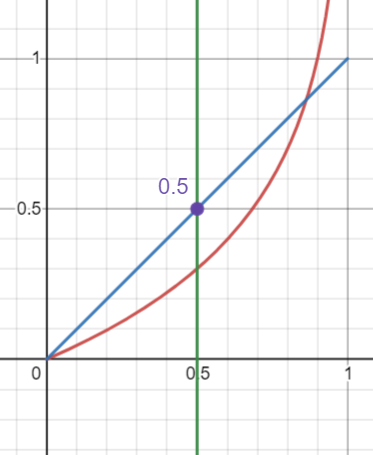
\includegraphics[width=5cm]{q32VisIntuition}
				\end{figure}
				In particular, for all $0 <x < 1/2$, we have $|\log(1-x)| -x > 0$, showing that $x$ is greater
				than $\log(1-x)$ for all $x \in (0,1/2)$.

				Then from here, this is a simple application of the Weiestrass $M$-test. Let $K = \sum_i^N
				\log(1-\alpha_i)$ to eliminate the irregular part. Then since $|\log(1-\alpha_i)| < \alpha_i$,
				for all $i > N$ and $\sum_i^\infty \alpha_i$ converges, by the Weiestrass $M$-test the $\sum_{i=N+1}^\infty
				\log(1-\alpha_i)$ converges. Let's say it converges to $L$. Then
				\[
					\sum_{i=1}^\infty \log(1-\alpha_i) = K + L > -\infty
				\]
				as we sought to show.
			\item[($\Rw$)] let $\prod (1-\alpha_i) > 0$ so equivalently $\sum_i^\infty \log(1-\alpha_i)
				> -\infty$ so $\sum_i^\infty \log(1-\alpha_i) = K$ for appropriate $K \in \R$. Then since the
				series converges, we have that
				\[
					eK = e\sum_i^\infty \log(1-\alpha_i) = \sum_i^\infty e\log(1-\alpha_i)
				\]
				i.e., we can scale the terms by $e$. We will show why this scaling is important in a moment;
				before we do we must setup a little more. 

				Since the series converges, it must be that $e\log(1-\alpha_i) \rw 0$. So pick $N$ such that
				for all $i > N$, $e\log(1-\alpha_i) < 1/2$. Then notice that $\alpha_i < e\log(1-\alpha_i)$.
				This is easier to see with a visual aid:
				\begin{figure}[H]
					\centering
					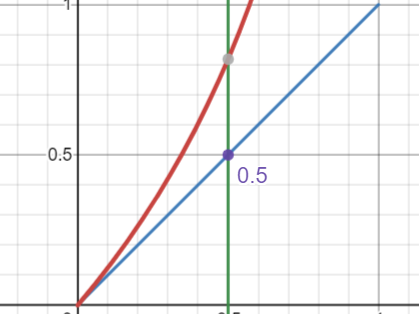
\includegraphics[width=5cm]{q32VisualIntuition2}
				\end{figure}

				Or, to carry out some of the computations, if you raise $e\log(1-\alpha_i) = \log(1-\alpha_i)e$ to the
				power of $e$, you get
				\[
					(e^{\log(1-\alpha_i)})^e  = (1-\alpha_i)^e \ge \alpha_i^e \quad \forall \alpha_i \in (0, 1/2]
				\]
				 and so the inequality holds. Then the proof continues as for the $\Lw$ direction by setting up an
				appropriate constant term to bound the irregularities, then using the Weiestrass $M$
				test bound every $\alpha_i$ by $\log(1-\alpha_i)$, and since $\sum_i^\infty
				\log(1-\alpha_i)$ converges, we get that $\sum_{i=N}^\infty \alpha_i$ also converge, and
				since it will be the sum of a constant plus the convergent value, $\sum_{i=1}^\infty
				\alpha_i$ converges, as we sought to show.
		\end{enumerate}

	Now, let $\beta$ be given. Let $x_i = \prod_{i=1}^n (1-\alpha_i)$. We'll construct a sequence where
	\[
		x_1 = \beta + \frac{1-\beta}{2} \qquad x_2 = \beta + \frac{1-\beta}{4} \quad\cdots\quad x_n = \beta
		+ \frac{1-\beta}{2^n} \cdots
	\]
	to accomplish this, let
	\begin{equation}\label{eq:2}
		\alpha_i = 1 - \frac{\beta + \frac{1-\beta}{2^i}}{\beta + \frac{1-\beta}{2^{i-1}}}
	\end{equation}
	This construction comes from solving the following equation:
	\[
		\left(\beta + \frac{1-\beta}{2}\right)y_2 = \beta + \frac{1-\beta}{4}\ \Rw\ y_2 = \frac{\beta
		+ \frac{1-\beta}{4}}{\beta + \frac{1-\beta}{2}}
	\]
	so $\alpha_2 = 1 - y_2$, and clearly $\alpha_2 \in (0,1)$ since the denominator is bigger than the
	numerator in the above calculations. Generalizing this pattern, we get the that $\alpha_i$ would be of the from
	presented in equation~(\ref{eq:2}) and $\alpha_i \in (0,1)$. Thus, we get that
	\[
		\lim_{n \rw \infty} \prod_i^n (1-\alpha_i) = \lim_{n \rw \infty} \beta + \frac{1-\beta}{2^n}
		= \beta
	\]
	as we sought to show
\end{Proof}

Now, let's say we are starting with $[0,1]$ but on each iteration eliminates intervals that sum to $\alpha_i$. Let $K_i$
be the $i$th step in this itteration. Notice that:
\[
	m(K_{i+1}) = (1-\alpha_i)m(K_i)
\]
Then by what we've just shown, we can make $K = \cap_i^\infty K_i$ be any value up to and including $0$ and $1$. 



\begin{prop}{All Cantor Set Homeomorphism}{allCantorSetHomeomorphism}
	Let $C_n$ be a cantor set where $m(C_n) = n$. Then $C_n \cong C_0$
\end{prop}

\begin{Proof}
	section 9 of Pugh -- will get back to it
\end{Proof}


You can also prove uncountability directly by making a string represent which side of the split interval you go to. TBD

Next, you might've seen many uncountable sets which are dense in $\R$. Here we have an absolutely facsinating result:
$C$ is \emph{nowhere dense in }$[0,1]$. 

\begin{defn}{Dense, Somwehre Dense, Nowhere Dense}{nowhereSomewhereDense}
	If $S \sse M$ and $\oln{S} = M$, then $S$ is dense in $M$. The set $S$ is somehwere dense if there exists an open
	nonemtpy set $U\sse M$ such that $\oln{S\cap U} \supset U$. If $S$ is not somwerhe dense, then it is \emph{nowhere
	dense}
\end{defn}

\begin{prop}{$C$ Nowhere Dense}{cNowhereDense}
	The Cantor set contains no interval and is nowehre dense in $\R$
\end{prop}


\begin{Proof}
	To prove it doens't contian an interval, assume it does, then chose an $n$ alrge enough, that is $(\frac{1}{3})^n
	< b-a$, so that it will not be in the interval. 

	For anowhere dense, assuem ti's somwerhe then, then $\oln{C\cap U}\supset U \supset (a,b)$ -- a contradiction.
\end{Proof}


We know present how Cantor sets are almost initial objects in compact metric space

\begin{thm}{Cantor Surjection Theorem}{cantorSurjectionorem}
	Given a compact nonempty metric space $M$. there is a continuous surjection of $C$ onto $M$
\end{thm}

\begin{Proof}
	In homeowkr, we proved this for $C \rw [0,1]$. Proof in Pugh. starts on p.108
\end{Proof}

Finally, we present how all cantor sets are homeomorphic. 

\begin{thm}{Moore-Kline Theorem}{mooreKlinethm}
	We say $M$ is a Cantor space if it is compact, nonempty, perfect, and totally disconnected (like the cantor set). 
	Every cantor sapce $M$ is homeomorphic to the standard middle-thirds Cantor set $C$.

	In other words, those properties \emph{define} Cantor sets.

\end{thm}

\begin{Proof}
	Pugh. p.112
\end{Proof}

\begin{cor}{Cantor And Fat Cantor Set}{cantorAndFatCantorSet}
	The fact Cantor set is homeomorphic to the standard Cantor set
\end{cor}

\begin{Proof}
	Using \ref{th:mooreKlinethm}, the result is immediate.
\end{Proof}

This is intersting, since it shows that meausre is \emph{not} a topological poperty! This should makes sense with
$(0,1)$ and $\R$ being homeomorphic with the same measures, but different, but this is an even more extreme example. 

\begin{cor}{Product Of Cantor Sets}{prodCantorSets}
	A cantor set is homeomorhic to its own cartesian product; $C\equiv C\times C$. 
\end{cor}

\begin{Proof}
	
\end{Proof}


A fact that Folland added that I thought was cool is that since every subset of the cantor set is Lebesgue Measurable
(since the cantor set has measure zero and the Lebesgue measure is complete), we have that 
\[
	|\EL| = |P(\R)| > \aleph_1\quad\text{but}\quad |\BB_\R| = \aleph_1
\]
so there are a \emph{tone} of zero-measure sets, however, we can essentially ignore them because they are zero measure
sets!!

\chapter{Integration}\label{cha:integration}

In this chapter, we now work with function's between measure spaces that preserve measure structure! I'll add more
intuition here later

Measurable functions are starting to feel like the types of functions we ``usually'' work with, the same way measurable
sets are the sets we ``usually'' work with. Being continuous can be a bit strong (ex. being a monotone function doesn't
imply continuous), but measureability rectifies that by in a sense expanding what are the possible ``pre-images'' we
allow to take (ex. Monotone functions \emph{are} always measurable, as we will demonstrate)

\section{Measurable Functions}

Recall that if $f: X \rw Y$ is a function, then $f^{-1}: P(Y) \rw P(X)$ is a function where $f^{-1}(E) = \set{x \in
X}{f(x) \in E}$ which preserves unions, intersections, and compliments. Thus, if $\EN$ is a $\sigma$-algebra on $Y$,
$f^{-1}(\EN)$ is a $\sigma$-algebra on $X$

\begin{defn}{Measurable Function}{measbleFunc}
	Let $f:X \rw Y$ be a function and $(X, \MM$) and $(Y, \EN)$ be measurable spaces. Then $f$ is called
	a $(\MM, \EN)$-\emph{measurable function} (or just measurable) if for all $E \in \EN$
	\[
		f^{-1}(E) \in \MM
	\]
\end{defn}

Just like in topology, this could be thought of as a surjection of the measurable space on $X$ onto the measurable space
on $Y$. It should be clear that the composition of two measurable functions is measurable, and that the identity
function is clearly a measurable function, and so the collection of measurable functions and measurable spaces from
a category, usually denoted \bf{Meas}. 

Just like lemma~\ref{lm:sigmaAlgGeneratingSetContainement} was useful for simplifying proofs, we proof the following:

\begin{lem}{Measurable Function and Generating Sets}{measFuncAndGenSet}
	Let $\EN$ be generated by $\CE$. Then $f: X \rw Y$ is a $(\MM, \EN)$-measurable function if and only if for all $E
	\in \CE$, $f^{-1}(E) \in \MM$
\end{lem}

\begin{Proof}
	The $\Rw$ direction a-fortiori true by definition. The $\Lw$ direction comes from $f^{-1}$ preserving unions and
	compliments, so $\set{E \sse Y}{f^{-1}(E) \in \MM}$ is a $\sigma$-algebra that contains $\CE$, and so contains
	$\EN$. 
\end{Proof}

From this, there is a very nice corrollary when $\MM$ is a collection of Borel sets:

\begin{cor}{Continuous Function $\Rw$ Measurable Function}{contThenMeasble}
	Let $f: X \rw Y$ be a continuous function. Then it is a measurable function. 
\end{cor}

\begin{Proof}
	Since $f$ is continuous, the pre-image of an open set (in particular, open intervals) is open, and hence by
	proposition~\ref{pr:generatorsForBorelSets} and lemma~\ref{lm:measFuncAndGenSet} it is measurable
\end{Proof}

Naturally, in analysis, the most important measurable functions will be of the form
\[
	f: \R \rw \R \qquad f: \R \rw \C
\]
In this case, we will \emph{always} assume the codomain will have $\BB_\R$ or $\BB_\C$ measure. In fact, if we have
a function $f: X \rw \R$ or $f: X \rw \C$, then we will sometimes say $f$ is $\MM$-measurable instead of $(\MM,
\BB_\C$-measurable. We sometimes distinguish between Borel and Lebesgue measurable for functions of the form $f: \R \rw
\C$ (resp. $f: \R \rw \R$. If it's Borel measurable, the domain has the $\BB_\R$ measure space, and $\EL$ if it is
Lebesgue measurable. 

\begin{titledBox}{Note: }
	Though the composition of two measurable sets is measurable, it does \emph{not} follow that the composition of two
	\emph{Lebesgue} measurable sets are Lebesgue measurable. see p.44 and homework exercise)
\end{titledBox}

\begin{example}{Measurable Functions}{measFuncEx}
	include the composition of two Lebesgue measurable need not be Lebesgue here. Include Monotone function. comment how
	naturally all continuous functions are also here. 
\end{example}

Just like for Borel sets earlier, we have the following equivalences

\begin{prop}{Borel sets and Measurable Functions}{borelsetsAndMeasFunc}
	Let $(X, \MM)$ be a measurable space and $f: X \rw \R$. Then the following are equivalent:
	\begin{enumerate}
		\item $f$ is $\MM$-measurable
		\item $f^{-1}((a, \infty))\in \MM$ for all $a \in \R$
		\item $f^{-1}([a, \infty))\in \MM$ for all $a \in \R$
		\item $f^{-1}((-\infty,a))\in \MM$ for all $a \in \R$
		\item $f^{-1}((-\infty,a])\in \MM$ for all $a \in \R$
	\end{enumerate}
\end{prop}

\begin{Proof}
	This was a 357 homework! In this book, it follows from proposition~\ref{pr:generatorsForBorelSets} and
	lemma~\ref{lm:measFuncAndGenSet}. 
\end{Proof}

Similarly, we will soon be encountering co-domains which are product spaces (ex. $\R^n$ or $\C^n$). In particular, let's
say we had some set $X$, and some family of measurable spaces $\{(Y_\alpha, \MM_\alpha\}_{\alpha \in A}$, and $f:
X \rw Y_\alpha$ is a map for each $\alpha \in A$. Then we can impose a unique smallest $\sigma$-algebra on $X$ that
makes each $f_\alpha$ a measurable function, in particular, $\MM_X = \set{f^{-1}_\alpha(E_\alpha)}{E_\alpha \in
\MM_\alpha,\ \alpha \in A}$. This $\sigma$-algebra on $X$ is called the \emph{$\sigma$-algebra generated by
$\{f_\alpha\}_{\alpha \in A}$}. 


\begin{prop}{Product of Measurable Functions}{measFuncProd}
	Let $(X, \MM)$ be a measurable space and $(Y_\alpha, \EN_\alpha)$ be a collection of measurable spaces, so $Y
	= \prod_{\alpha \in A} Y_\alpha$, $\EN = \bigotimes_{\alpha \in A} \EN_\alpha$, and $\pi_\alpha: Y \rw Y_\alpha$ is
	the coordinate map. Then $f: X \rw Y$ is $(\EM, \EN)$-measurable if and only if $f_\alpha = \pi_\alpha \circ f$ is
	$(\EM, \EN_\alpha)$-measurable. 
\end{prop}

\begin{Proof}
	Let's say $f$ is $(\EM, \EN)$-measurable. Then since the composition of two measurable functions is measurable, so
	are each $f_\alpha$ is measurable (since $\pi_\alpha$ is measurable by proposition~\ref{pr:borelsetsAndMeasFunc}). 

	Conversely, if every $f_\alpha$ is $(\EM, \EN_\alpha)$-measurable, then for each $E_\alpha \in \EN_\alpha$,
	$f^{-1}(\pi_\alpha^{-1}(E_\alpha)) = f^{-1}(E_\alpha) \in \EM$, and since these sets generate $\MM$, we have that
	$f$ is $(\EM, \EN$)-measurable by proposition~\ref{pr:borelsetsAndMeasFunc}
\end{Proof}

This proposition also let's us define what it means to take the ``product'' of two functions. As a consequence, we can
give an easy criterion for when complex functions are measurable:

\begin{cor}{Complex Function Measureability}{complexFuncMeasble}
	Let $f: X \rw \C$ be a complex function. Then $f$ is $\EM$-measurable if and only if $\Re f$ and $\Im f$ are both
	measurable.
\end{cor}

\begin{Proof}
	This is simply taking advantage of the topology of $\C$, namely
	\[
		\BB_\C = \BB_{\R^2} \overset{!}{=} \BB_\R\otimes \BB_\R
	\]
	where the $\overset{!}{=}$ equality comes from the fact that $\R$ is separable (see
	proposition~\ref{pr:borelSetsandMetricSp}). And so proposition~\ref{pr:measFuncProd} completes the proof.
\end{Proof}

Sometimes, we want to work with the extended real line (or in general some compactification of a topological space). If
$\oln\R = [-\infty, \infty]$, Then let 
\[
	\BB_{\oln\R} = \set{E \sse \oln\R }{E\cap \R \in \BB_\R}
\]
Notice that is we put the metric $\rho$ on $\oln\R$ to be $\rho(x,y) = |\tan^{-1}(x) -\tan^{-1}(y)|$, then
$\BB_{\oln\R}$ is indeed the usual definition of a Borel $\sigma$-algebra (exercise)

Next, if the codomain has some notion of $+$ and $\cdot$, we establish that the basic ``$\C$-algebra operations'' work on measurable functions:

\begin{prop}{Arithmetics on Measurable Functions}{measFuncArithmetics}
	Let $f: X \rw \C$ and $g: X \rw \C$ be $\EM$-measurable functions. Then $f+g$, $fg$, and $zf$ for $z \in \C$ are $\EM$-measurable
	functions
\end{prop}

Note that we have limited ourselves to $\C$. This still works with $\oln\R$ with the appropriate care of the
$\infty-\infty$ and $0\cdot \infty$ case (exercise 2 in book)

\begin{Proof}
	Since $f$ and $g$, are measurable, then their ``cartesian product'' is measurable by
	proposition~\ref{pr:measFuncProd}
	\[
		F: X \rw \C\times \C \qquad F(x) = (f(x), g(x))
	\]
	In particular, $F$ is $(\EM, \BB_\C\otimes \BB_\C)$-measurable. Next, consider $p: \C\times \C \rw \C$, $p(x,y)
	= x+y$ and $t: \C\times \C \rw \C$, $t(x,y) = xy$ ($p$ for plus, $t$ for times). Then since $p$ and $t$ are
	continuous, by corrollary~\ref{co:contThenMeasble} $p$ and $t$ are $(\BB_{\C\times \C}, \BB_\C)$-measurable. Thus,
	$p\circ F$ and $t\circ F$ is $(\EM, \BB_\C)$-measurable, and by definition
	\[
		f+g = p\circ F\qquad fg = t\circ F
	\]
	completing the proof
\end{Proof}

Next, we show that $\sup$, $\inf$, $\limsup$ and $\liminf$ are all preserved under measurability

Comment here for future reference: % https://math.stackexchange.com/questions/1131461/if-f-n-are-measurable-and-f-n-to-f-almost-everywhere-then-f-is-measurable#1133946

\begin{prop}{Measurable functions and Limit Bounding}{measFuncAndSup}
	Let $f_i: X \rw \oln\R$ be $\EM$-measurable functions for each $i$ and consider $\{f_i\}_{i=1}^\infty$. Then
	\[
		g_1(x) = \sup_i f_i(x) \qquad g_2(x) = \inf_i f_i(x)
	\]
	\[
		g_3(x) =\limsup_{i \rw \infty} f_i(x)  \qquad g_4(x) = \liminf_{i \rw \infty} f_i(x)
	\]
\end{prop}

The codomain $\oln\R$ was used so that the sup and inf is still considered defined if $\sup = \pm \infty$ or $\inf = \pm
\infty$. 

Also, recall that
\[
	\sup_i f_i(x) = \sup \set{f_i(x)}{i \in \N}
\]
and so this expression means we're taking the set $f_i(x)$ for each $i$ and taking the sup of that set. In other words,
for every point $x$ we're taking the supremum of the set $\{f_1(x), f_2(x), ...\}$. Symmetrically
the same for $\inf$. For $\limsup$, recall that:
\[
	\limsup_i f_i(x) = \lim_{i \rw \infty} \sup\set{f_k(x)}{k \ge i}
\]
that is, we are constantly shrinking the set over which we are doing the supremum, which in a sense means we're trying
to ``hug'' the value from above as close as possible. Symmetrically the same for $\liminf$. If you're visual, I like to
keep this image in mind: Let's say the blue line is the value of $f_i(x_0)$ for a specified $x_0$. Then:

\begin{figure}[H]
	\centering
	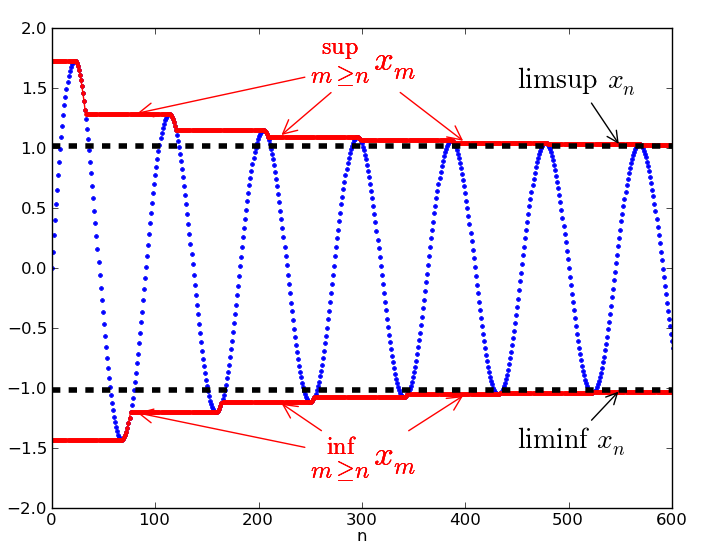
\includegraphics[width=10cm]{limsup}
\end{figure}


\begin{Proof}
	To show $\sup_i f_i$ and $\inf_i g_i$ are measurable, we will do a very clever trick: notice that:
	\[
		g_1^{-1}((a, \infty]) = \bigcup_i^\infty f_i^{-1}((a, \infty]) \qquad g_2^{-1}(-\infty, a])) = \cup_i^\infty
		f_i^{-1}([-\infty, a))
	\]
	since the pre-image of rays going off to infinity must contain and so $g_1$ and $g_2$ are measurable by proposition~\ref{pr:borelSetsandMetricSp}. Next, let 
	\[
		h_k(x) = \sup_{i > k} f_i(x) = \sup\set{f_k(x)}{k > i}
	\]
	then by what we've just established, $h_k$ is measurable for each $k$. Then by construction:
	\[
		g_3 = \inf_k h_k
	\]
	and so $g_3$ is measurable (notice that we applied $\inf$ to $h_k$). Similarly for $g_4$. 

\end{Proof}

as an immediate corrollary

\begin{cor}{}{maxMinMeasurable}
	Let $f,g$ be measurable functions. Then so is $\max\{f,g\}$ and $\min\{f,g\}$
\end{cor}

\begin{cor}{Measurable Preserved under Pointwise limit}{measFuncPointLimt}
	Let $\{f_i\}$ be a sequence of measurable function. If $\lim_{i \rw \infty} f_i(x)$ exists for every $x$, and we define $f: X \rw \oln\R$ to be 
	\[
		f(x) = \lim_{i \rw \infty} f_i(x)
	\]
	then $f$ is measurable (i.e. point-wise convergence preserves measureability)
\end{cor}

Recall that point-wise convergence \emph{does not preserve continuity} (the steeple function's are the usual example).
However, measureability is sufficiently general to be preserved under this weaker form of convergence! Naturally, if the
sequence of functions $\{f_i\}$ are all $\EM$-measurable and uniformally convergent, they are measurable

\begin{Proof}
	If $f$ exists (i.e., every $f_n(x)$ converges pointwise to $f(x)$), then by
	proposition~\ref{pr:measFuncAndSup}, $f = g_3 = g_4$, completing the proof.
\end{Proof}

With this in mind, we will write introduce some new notation which will soon become useful when defining integrable
functions. 

\begin{defn}{Real and Complex Decomposition}{realComplexDecomp}
	Let $f:X \rw \R$ and $g: X \rw \C$ be real and complex measurable functions respectively. Then
	\[
		f^+ = \max\{f, 0\} \qquad f^- = \max\{-f, 0\}
	\]
	and
	\[
		\sgn(g(x)) = \begin{cases}
			\frac{g(x)}{|g(x)|} & g(x) \ne 0\\
			0 & g(x) = 0
		\end{cases}
		\qquad
		|g(x)| = |z| = |x+iy| = \sqrt{x^2 + y^2}
	\]
	which gives the decomposition of:
	\[
		f = f^+ - f^-$, $g = (\sgn g)|g|
	\]
\end{defn}

The functions $f^+$ and $f^-$ are clearly well-defined and measurable. For the complex case, $|\cdot|$ is continuous everywhere and $z \mapsto \sgn z$
is continuous everywhere except $0$. It is measurable since if $U \sse \C$ is open, then $\sgn^{-1}(U)$ is either $V$
for some open set $V$, or $V\cup \{0\}$, meaning $\sgn$ is Borel measurable.

In some textbooks, $\operatorname{arg}$ is used instead of $\sgn$. 

\subsection{Standard Representation}

We now how that every measurable function is in fact simply the limit of a bunch of easy to work with function, in
particular, linear combination of characteristic functions! As a reminder, if $\chi_E: X \rw \R$ (or $\{0,1\}$) where $E \sse X$ and
\[
	\chi_E(x) = \begin{cases}
		1 & x \in E\\
		0 & x \notin E
	\end{cases}
\]
Then $\chi_E$ is called the characteristic (or indicator) function. It is sometimes also denoted as $1_E$ or $I_E$. 

\begin{defn}{Simple function}{simpleFunc}
	Let $E_i \sse \C$ be some finite collection of sets. Then the finite linear combination of characteristic functions
	on $E_i$ multiplied by a complex constant:
	\[
		f = \sum_{i=1}^n z_i\chi_{E_i}
	\]
	is called a \emph{simple function}
\end{defn}

\begin{example}{Simple Functions}{simplFuncEx}
	\begin{enumerate}
		\item Show that $|f(X)| < \infty$ then $f$ is in fact a simple function (hint: let $E_i = z_i$ for each $z_i \in f(X)$).
			In fact, each coefficient can also be distinct (let it be the respective $z_i$ from the range)
		\item Show that if $f$ and $g$ are simple functions, so are $f+g$ and $fg$ 
	\end{enumerate}
\end{example}

Using these, we can now show that any measurable function is simply the limit of simple functions!

\begin{thm}{Simple Function Approximation}{measFuncSimpleRep}
	Let $(X, \EM)$ be a measurable space. Then
	\begin{enumerate}
		\item If $f: X \rw [0,\infty]$ is measurable, there exists a sequence of functions $\{\phi_i\}_{i=1}^\infty$
			such that 
			\[
				0 \le \phi_1 \le \phi_2 \le \cdots \le f
			\]
			where $\lim_{n \rw \infty} \phi_i(x) = f(x)$ (i.e. $\phi_n \rw f$ pointwise). and $\phi_n \rightrightarrows
			f$ on a bounded domain (i.e. uniformally converges)
		\item If $f: X \rw \C$ is measurable, there exists a sequence of functions $\{\phi_i\}_{i=1}^\infty$
			such that 
			\[
				0 \le |\phi_1| \le |\phi_2| \le \cdots \le |f|
			\]
			where $\lim_{n \rw \infty} \phi_i(x) = f(x)$ (i.e. $\phi_n \rw f$ pointwise). and $\phi_n \rightrightarrows
			f$ on a bounded domain (i.e. uniformally converges)
	\end{enumerate}
\end{thm}

\begin{Proof}
	This was a 357 hw! Essentially, you will get indicator functions to converge to the value like so:
	\begin{figure}[h]
		\centering
		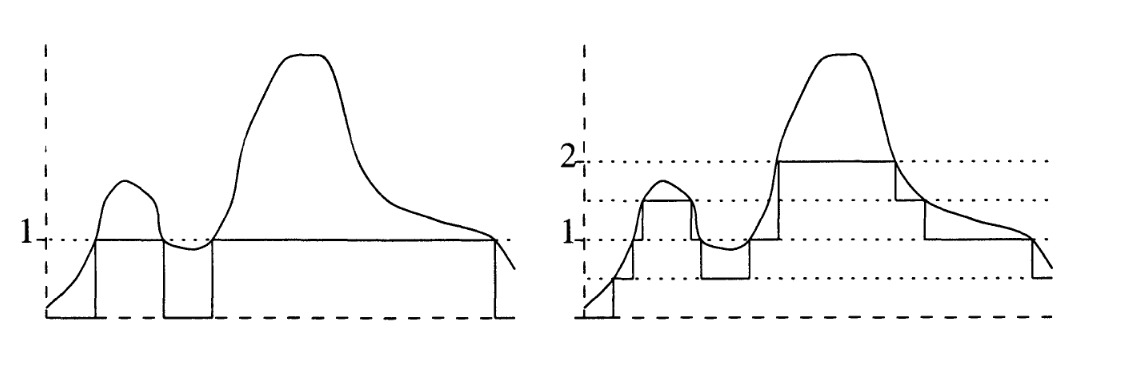
\includegraphics[width=10cm]{indicatorApprox}
	\end{figure}
	In particular, for $n \in \N_{\ge 0}$ and $0 \le k \le 2^{2n}-1$, let
	\[
		E_n^k  = f^{-1}\left( \left(\frac{k}{2^n}, \frac{k+1}{2^n}\right)\right) \qquad F_n = f^{-1}((2^n, \infty])
	\]
	and
	\[
		\phi_n = \sum_{k=0}^{2^{2n}-1} \frac{k}{2^n} \chi_{E_n^k} 2^n\chi_{F_n}
	\]
	then we get that $\phi_n \le \phi_{n+1}$ for all $n$ and $0 \le f-\phi_n \le \frac{1}{2^n}$ where $f\le 2^n$. The
	rest is left to check. 

	Generalizing to $\C$, decomposing to $f = g + ih = (g^+ + g^-) = i(h^+ + h^-)$, where the $+$ and $-$ functions are
	the positive and negative parts of $f$ and $g$, then we can repeat the process for each of these and get $\psi_n^+,
	\psi_n^-, \zeta_n^+, \zeta_n^-$ and let $\phi_n = (\psi_n^+ - \psi_n^-) + i(\zeta_n^+ - \zeta_n^-)$. 
\end{Proof}

Given this, we get a powerfull way of being able to deduce one function is measurable it is equal to a measurable
function up to a zero-measure set (if the measure $\mu$ is complete)

\begin{prop}{Measurability up to Zero Set}{measUpToZeroSet}
	Let $(X, \EM, \mu)$ and $(Y, \EN, \nu)$ be two measure with $\nu$ being a complete measure, and let $f: X \rw Y$ be
	$(\EM, \EN)$-measurable. Then:
	\begin{enumerate}
		\item If $f = g$ up to a zero measure set with respect to $\mu$ (shorthanded to $\mu$-a.e.), then $g$ is measurable
		\item If $f_n$ is measurable for each $n \in \N$ and $f_n \rw f$ $\mu$-a.e, then $f$ is measurable
	\end{enumerate}
\end{prop}


\begin{Proof}
	\begin{enumerate}
		\item Let's say $N$ were the points in $X$ such  
			%I have two proofs for this fact:

			%Take advantage that $f$ has a sequence of simple functions that converges to it. Let $N$ be the set of
			%points in $Y$ that are in the codomain of $g$ and do not match $f$. By assumption $\nu(N) = 0$. Then any
			%subset of $N$ has measure $0$. That also means that if $E$ is a measurable function, $E \setminus F$ where
			%$F \sse N$ is also measurable, and so the simple functions for $f$ can be modified to indicate over
			%$E_i^j\setminus F$. Then, some indicator functions can be made for $N$ so that $\phi_1 \le \phi_2 \le \sdots
			%\le f$ is preserved. 

			Secondly, 
		\item Since $f_n \rw f$ a.e. then $\limsup f_n = \liminf f_n$ a.e., i.e. for every point such Taft $\limsup
			f_n(x) \ne \liminf f_n(x)$, put them in the set $N$, and $\nu(N) = 0$. Since $N$ is measurable, 
	\end{enumerate}
	exercise 10 in book
\end{Proof}

However, if $\mu$ is not complete, it turns out to make little difference since we can complete the measure, produce the
result, and restrict back to the original measure without changing the result:
\begin{prop}{}{muAE}
	Let $(X, \MM, \mu)$ be a measure sapce and $(X, \oln\EM, \oln\mu)$ be its completion. if $f$ is
	a $\oln\EM$-measurable function on $X$, there is a $\EM$-measurable function $g$ such that $f = g$ $\oln\mu$-a.e.
\end{prop}

\begin{Proof}
	If $f$ is a simple function, then we see that the completion will at most remove finitely many points when we
	restrict every $\chi_E$ ($E \in \oln\MM$) to $g$, and so $f = g$ $\oln\mu$-a.e. 

	Now let $f$ be a $\oln\MM$-measurable function, and by theorem~\ref{th:measFuncSimpleRep} choose a sequence of $\oln\MM$-measurable functions
	$\{\phi_i\}_{i=1}^\infty$ that converge pointwise to $f$. The idea is that each $\phi_i = \psi_i$ $\oln\mu$-a.e.,
	that is, there exists a $E_i$ where $\phi_i(x) \ne \psi_i(x)$ for all $x \in E_i$ but $\oln\mu(E_i) = 0$, and the
	countable union of these will still be measure $0$. 

	In particular Let $E = \bigcup_i^\infty E_i$. By definition of completion, there must exist some $N$ such that
	$\mu(N) = 0$ and $E \sse N$. Let $g = \lim_{\chi_X- N}\psi_n$. Then $g$ is measurable by
	corollary~\ref{co:measFuncPointLimt}, and clearly $f = g$ on $N^c$, completing the proof.
\end{Proof}




\section{Integration of non-negative Function}

We are now in a position to how to integrate functions (integrable coming soon)! Throughout this section, let $(X, \EM, \mu)$ be a measure space

\begin{defn}{$L^+$}{measbleFuncSp}
	Let 
	\[
		L^+ = \set{f: X \rw [0, \infty]}{\text{$f$ is a $\EM$-measurable function}}
	\]
\end{defn}

Sometimes, $L^+$ is written as $L^+(X)$, $L^+(\mu)$, or $L^+(\mu, X)$ to emphasize which space of functions we are
dealing with. If it is unambiguous, we use $L^+$. 

\begin{defn}{Integral of Simple Function}{intOfSimpleFunc}
	Let $f = \sum_1^n a_i\chi_{E_i}$ be a simple function. Then define the \emph{integral of $f$ with respect to $\mu$} to be
	\[
		\int fd\mu = \sum_i^n a_i\mu(E_i)
	\]
\end{defn}

In other words, we simply took the measure of the domain of $\chi_{E_i}$ for each $i$. As usual, we take the convention
that $0\cdot \infty = 0$. We will also allow $\int f = \infty$ to be a valid result. If there is no confusion, we will
write $\int f$ instead of $\int fd\mu$. It should also be emphasized that it is the measure of the \emph{domain} and the
coefficient from the \emph{codomain} that we are taking. 

If we want to integrate over just some $A \sse X$ where $A \in \EM$, then $\left.\phi\right|_{A}$ is also a simple
function (simply take $\chi_{E\cap A}$ for each characteristic function). We usually denote this by
\[
	\int_A fd\mu = \int f\chi_A\, d\mu
\]
Because of this notation, we can write $\int fd\mu$ as 
\[
	\int f d\mu = \int_X fd\mu
\]

\begin{prop}{properties of Integrals of Simple Functions}{propIntofSimplFunc}
	Let $\phi$ and $\psi$ be simple functions in $L^+$. Then
	\begin{enumerate}
		\item if $c \ge 0$, $\int c\phi d\mu = c\int \phi d\mu$
		\item $\int(\phi + \psi)d\mu = \int \phi d\mu + \int \psi d\mu$
		\item if $\phi \le \psi$ then $\int \phi \le \int \psi$
		\item The map $A \mapsto \int_A \phi d\mu$ is a measure on $\EM$ (TBD on the $\phi$ being where it is)
	\end{enumerate}
\end{prop}

\begin{Proof}
	Do these as midterm exercises
\end{Proof}


With this definition, we can define integrable function more generally:

\begin{defn}{Integral of Measurable Function}{intOFMeasFunc}
	Let $f \in L^+$. Then define
	\[
		\int f d\mu := \sup\set{\int \phi d\mu}{\text{$\phi$ is a simple function, }0 \le \phi \le f}
	\]
\end{defn}

It's important to see why the integral of a simple function will give the same result as the ``simple integral'' (i.e.
integral over simple functions from earlier), in particular since the set over which we are containing the supremum will
contain the simple function in question, and so the maximum will be achieved by itself (and proposition 2.13c?).
Furthermore, results 1 and 3 from proposition~\ref{pr:propIntofSimplFunc} holds for the definition of integration just
given. The other results, in particular linearity, will be established soon.

Given the supremum definition of the integral, it could be rather hard to find the integral of a function in $L^+$. We
essentially never check this, and treat the following theorem as the de-facto way of finding the integral:

\begin{thm}{Monotone Convergence Theorem (MCT)}{mct}
	If $\{f_n\}_{i=1}^\infty \sse L^+$ is a sequence such that $f_i \le f_{i+1}$ for all $i \in \N$ and $f = \lim_{n \rw
	\infty} f_n$ $(=\sup_n f_n)$, then
	\[
		\int f = \lim_{n \rw \infty}\int f_n
	\]
	or, since $f = \lim_{n \rw \infty} f_n$:
	\[
		\int \lim_{n \rw \infty} f = \lim_{n \rw \infty}\int f_n
	\]
\end{thm}

Note that this is \emph{not} the theorem saying we can move limits through the integral in general (we need more
build-up to sate such a result), but rather it is saying that if we have an non-decreasing sequence, then the limit
seems like it can ``move through'' the integral, but in reality we are just equating two results (which I guess is
what always happens, but somehow clarifying this in my mind feels useful)

\begin{Proof}
	We'll show $\le$ and $\ge$. For $\le$, notice that $\{\int f_n\}$ is an increasing sequence, and so converges
	(possibly to $\infty$). Furthermore, $f_n \le f$ for all $n$, and so by
	proposition~\ref{pr:propIntofSimplFunc} updated for general integral functions, we have:
	\[
		\int f_n \le \int f
	\]
	and so 
	\[
		\lim_{n \rw \infty} \int f_n \le f
	\]

	Conversely, we'll show that if we ``shrink'' the left hand side by a factor of $\alpha \in(0,1)$ so that we get
	$\ge$, then since this will be true for all $\alpha$, we will get the result we want. 

	Fix some $\alpha \in (0,1)$, and choose a simple function where $0 \le \phi \le f$ (such a function exists by
	theorem~\ref{th:measFuncSimpleRep}). Let
	\[
		E_n = \set{x \in \oln\R}{f_n(x) \ge \alpha\phi(x)}
	\]
	Then $\{E_n\}_{n=1}^\infty$ is an increasing sequence (via inclusion) of measurable sets who's union if $X$ (since
	$\lim_{n \rw \infty} f_n = f$ and the $f_n$'s are increasing). Then
	\[
		\int f_n \ge \int_{E_n} f_n \ge \alpha\int_{E_n} \phi
	\]
	Since the map $E_n \mapsto \int_{E_n} \phi$ is measurable by proposition~\ref{pr:propIntofSimplFunc} and the $E_n$'s
	are continuous from above, we have
	\[
		\int_{E_n} \phi = \int \phi
	\]
	and so
	\[
		\lim_{n \rw \infty} \int f_n \ge \alpha\int \phi
	\]
	Since this is true for all $\alpha < 1$, it is true for $\alpha = 1$, and so $\int f_n \ge \int \phi$. Taking the
	supremum over all $\phi$, we get that
	\[
		\lim_{n \rw \infty} \int f_n \ge \int f
	\]
	And since we showed the $\le$ direction, we in fact have:
	\[
		\lim_{n \rw \infty} \int f_n = \int f
	\]
	as we sought to show
\end{Proof}

Thus, to find the value of $\int f$, it suffices to find some sequence of simple functions $\{\phi_n\}$ that converges
to $f$, which always exists since every measurable function has a standard representation
(theorem~\ref{th:measFuncSimpleRep}).

An immediate consequence of the Monotone Convergence Theorem is that linearity also applies to integrals:

\begin{prop}{Linearity of Integrals}{linearityofInt}
	Let $\{f_i\}_{i=1}^N \sse L^+$ where $N \in \N \cup \{\infty\}$ and let $f = \sum_i^N f_i$. Then
	\[
		\int f =  \sum_i^N \int f_n
	\]
\end{prop}

\begin{Proof}
	Let's first consider the case where $n = 2$ so that we have $f_1$ and $f_2$. Let $\{\phi_i\}$ and $\{\psi_i\}$ be
	a sequence for the standard representation of $f_1$ and $f_2$. Then clearly $\{\phi_i + \psi_i\}$ is a sequence for
	a standard representation of $f_1 + f_2$. Then by the Monotone Convergence Theorem
	\begin{align*}
		\int f_1 + f_2 &= \lim_{i \rw \infty} \int \phi_i + \psi_i\\
					   &\overset{\text{MCT}}{=} \int \lim_{i \rw \infty} \phi_i + \psi_i\\
					   &= \int \lim_{i \rw \infty} \phi_i +\lim_{i \rw \infty} \psi_i\\
					   &= \int \lim_{i \rw \infty} \phi_i +\lim_{i \rw \infty} \psi_i\\
					   &= \int \lim_{i \rw \infty} \phi_i +\int \lim_{i \rw \infty} \psi_i\\
					   &\overset{\text{MCT}}{=} \lim_{i \rw \infty}\int  \phi_i +\int \lim_{i \rw \infty} \psi_i\\
					   &= \int f_1 + \int f_2
	\end{align*}

	By induction, it holds that 
	\[
		\int \sum_i^n f_i = \sum_i^n \int f_i
	\]
	Letting $n \rw \infty$, we can once again apply the Monotone Convergence Theorem and get
	\begin{align*}
		\int \sum_i^\infty f_i &=\int \lim_{n \rw \infty} \sum_i^n f_i\\
							   &\overset{\text{MCT}}{=}\lim_{n \rw \infty} \int \sum_i^n f_i\\
							   &= \lim_{n \rw \infty} \sum_i^n \int f_i\\
							   &= \sum_i^\infty \int f_n
	\end{align*}
	completing the proof
\end{Proof}

The next result is a generalization from the same result with Riemann integrals, except we replace the condition of
``finitely many points'' with ``null-set amount of points''

\begin{prop}{Zero Integral}{zeroIntIFFmeas0AE}
	Let $f \in L^+$. Then $\int f = 0$ if and only if $f = 0$ a.e.
\end{prop}

\begin{Proof}
	Starting with simple functions, this is evident in both directions. If $\phi$ was our simple function and $\int \phi
	= 0$, then $\sum_i^n a_i\mu(E_i) = 0$, so either each $a_i = 0$ or each $\mu(E_i) = 0$ which immediately implies
	$\phi$ is zero a.e. (in fact, it is only measure zero). Conversely, if each $\mu(E_i) = 0$, then clearly
	$\int \phi = 0$. 

	Moving onto to a measurable function $f$, the $\Lw$ comes almost immediately. If $f = 0$ a.e., then for every simple
	function $\phi \le  f$, then $\phi = 0$ a.e., which we have established means $\int \phi = 0$. Then by definition of
	$\int f$:
	\[
		\int f = \sup_{\phi \le f} \int \phi = 0
	\]
	For the $\Rw$ direction, assume that $\int f = 0$, and for the sake of contradiction let's say $f \ne 0$ a.e. Let
	\[
		\bigcup_i^\infty E_n =\bigcup_i^\infty \set{x}{f(x) > \frac{1}{n}} = \set{x}{f(x) > 0} = E
	\]
	Since $f \ne 0$ a.e., it must be that $\mu(E) > 0$, and so by construction $\mu(E_n) > 0$. But then
	\[
		f \ge n^{-1}\chi_{E_n} \LRw \int f \ge n^{-1}\mu(E_n) > 0
	\]
	so the supremum of values in $f$ contain simple functions of nonzero measure, showing that $\int f > 0$ --
	a contradiction to our original assumption. 
\end{Proof}

This theorem let's us upgrade the Monotone Conversely Theorem by needing the convergence to happen up to a measure zero
set:

\begin{cor}{MCT a.e.}{mctAE}
	Let $\{f_n\}_{i=1}^\infty \sse L^+$ and $f \in \L^+$. Then if $f_1 \le f_2 \le \cdots \le f$ and $f_n \rw f$ a.e.,
	then 
	\[
		\int f = \lim_{n \rw \infty} \int f_n
	\]
\end{cor}


\begin{Proof}
	Let $f_n(x) \rw f(x)$ for all $x \in E$ such that $\mu(E^c) = 0$. Then $f - \left.f\right|_E = 0$ a.e. which implies
		$f_n - \left. f_n\right|_E = 0$ a.e., so by the Monotone Conversely Theorem
		\[
			\int f = \int \left. f\right|_E \overset{\text{MCT}}{=} \lim_{n \rw \infty}\int \left.f_n\right|_E = \lim_{n
					\rw \infty}\int f_n
			\]
			as we sought to show.
\end{Proof}

We next address the fact that the sequence $\{f_i\}$ must be increasing (at least a.e.) for the MCT. If it were not,
then it need not be the case that the limit passes through the integral!

\begin{example}{not increasing $\not\Rw$ Limit commutes with $\int$}{nonIncreasingCoutnerExampleMctEx}
	Let $X = R$ and $\mu$ be the Lebesgue measure. Consider the two following examples:
	\[
		\{n\chi_{(0, 1/n)}\}_{n=1}^\infty
	\]
	then it is clear that $n\chi_{(0, 1/n)} \rw 0$. However, notice that $\int n\chi_{(0, 1/n)} = 1$ for each element in
	the sequence. Thus:
	\[
		0 = \int \lim_{n \rw \infty} n\chi_{(0, 1/n)} \ne \lim_{n \rw \infty}\int n\chi_{(0, 1/n)} = 1
	\]
	Even if the function is bounded, the problem remains: take $\chi_{(n, n+1)}$ which also converges pointwise to $0$
	but the sequence of the integrals of the functions is a sequence of constants $1$ and so converges to $1$ which is
	clearly not $0$.

	Notice that in both examples, there is some ``escaping to infinity'' going on. We address this when talking about
	the Dominated Convergence Theorem in the next section. 
\end{example}


However, not all hope is lost; there is weakening to only the $\liminf$ and the equality to $\le$ which works in the
general case:

\begin{thm}{Fatou's Lemma}{fatouLem}
	If $\{f_n\} \sse L^+$ is \emph{any} sequence, then
	\[
		\int \liminf_n f_n \le \liminf_n \int f_n
	\]
\end{thm}

This is interesting if we interpret it from a sort of ``physics'' perspective: somehow, we have ``lost our mass'' in the
process of taking our limit. What Fatou's lemma is giving us is a measure of how we might bound this loss of mass. There
In fact, there are essentially 3 ways we can ``lose mass', the first two begin the counter-examples above, the last one
being a function that oscillates faster and faster (this last one requires a function that is also defined in the
negative, and so we will get back to this).

\begin{Proof}
	This comes directly from properties of the $\liminf$. Let $k \ge 1$. Then 
	\[
		\inf_{i \ge k} \le f_i \le f_j \quad \forall\ j \ge k
	\]
	Then by theorem~\ref{pr:propIntofSimplFunc}
	\[
		\int \inf_{i \ge k}\le \int f_i\quad \forall j \ge k
	\]
	and since this holds for all $j \ge k$, we get:
	\[
		\int \inf_{i \ge k}\le \inf_{j \ge k}\int f_i
	\]
	Since the $\liminf$ defines an increasing sequence of function, by letting $k \rw \infty$ and applying the Monotone
	Conversely Theorem:
	\[
		\int \liminf f_n = \lim_{k \rw \infty} \int \inf_{n \ge k} f_n \le \liminf \int f_n
	\]
	as we sought to show
\end{Proof}


Like before, the result holds if we loosen the condition so that $f_n \rw f$ a.e.

\begin{cor}{Fatou's Lemma a.e.}{fatouLemAE}
	let $\{f_n\} \sse L^+$ be any sequence and $f \in L^+$. If $f_n \rw f$ a.e. Then
	\[
		\int f \le \liminf_n \int f_n
	\]
\end{cor}

\begin{Proof}
	Using proposition~\ref{co:mctAE}, make  $f_n \rw f$ everywhere arguing that it is equivalent to do so, and then the
	rest is Fatou's Lemma. 
\end{Proof}

Finally, there is this result which I think is for some future proof:

\begin{prop}{}{propOfFiniteInt}
	Let $f \in L^+$. If $\int f < \infty$, then $\set{x}{f(x) = \infty}$ is a null set and $\set{x}{f(x) > 0}$is
	$\sigma$-finite
\end{prop}

\begin{Proof}
	was left as an exercise to the reader in the book
\end{Proof}


\section{Integration of Real and Complex Functions}

We'll again let $(X, \EM, \mu)$ be the fixed measure space for this section, except the codomain now will be either $\R$
or $\C$. 

For the case of $\R$, we can quickly extend our results from last section by splitting $f$ into $f^+$ and $f^-$ (which
are both measurable if $f$ is by corrollary~\ref{co:maxMinMeasurable}), and if at least one of $f^+$ or $f^-$ is finite,
then
\[
	\int f = \int f^+ -\int f^-
\]
Notice that if they are both minus we have $\infty - \infty$ which is in general not well-defined. Thus, we will limit
our attention to functions where $\int |f| < \infty$ since $|f| = f^+ + f^-$:

For the case of $\C$,  using the triangle inequality we get that:
\[
	|f| = |\Re f + \Im f| \le |\Re f| + |\Im f| \le f|f|
\]
and so both $\Re f$ and $\Im f$ and so we get non-trivial results if each value is finite. In that case, we define
\[
	\int f := \int \Re f + i\int \Im f
\]
We give a name over $\C$ (and with in the special case $\R$) that satisfy this finiteness condition:
\begin{defn}{Integrable Function}{intgbleFunc}
	Let $f:X \rw \C$ be measurable. We say $f$ is \emph{integrable} if 
	\[
		\int |f| < \infty
	\]
	Let $L^1$ represent the set of all integrable functions. 
\end{defn}

If the codomain is $\R$, then we get that $\int |f^+| < \infty$ and $\int |f^-| < \infty$, as we claimed for our
extension of the integral to $\R$. Similarly for $\C$. Furthermore, for any $E \in \EM$, we will say that $f$ is
\emph{integrable on $E$} if $\int_E |f| < \infty$.

The set of $L^1$ functions are well-behaved under addition and scalar multiplication in the sense that they form
a vector-space:

\begin{prop}{Vector Space on $L^1$}{L1VecSp}
	Let $L^1$ be the set of integrable functions. Then with $+$ and scalar multiplication, $L^1$ forms a vector-space
	(over $\R$ or $\C$ respective to the codomain). Furthermore, $\int$ is a linear functional on $L^1$ (i.e. $\int: L^1 \rw \R$ is a linear functional)
\end{prop}

\begin{Proof}
	the proof that $cf + dg$ is bounded comes from the triangle inequality and that $|cf| = |c||f|$. The fact that $cf
	\in L^1$ for any $c \in \R$ comes from proposition~\ref{pr:propIntofSimplFunc} and $f+g \in L^1$ comes from
	manipulating the definition using the linearity of the integral. 

	The fact that $\int $ is a linear functional (i.e. $\int f+g = \int f+ \int g$ and $\int cf = c\int g $) comes
	straight from our previous propositions. 
\end{Proof}

Next, we would like to establish some properties of integrable functions, including a useful inequality, and as in the
previous statement, two integrals are equal if $f = g$ a.e. Furthermore, the set of all ``interesting'' points (points
where $f(x) = 0$) have a very nice finiteness property:

\begin{prop}{Properties of Integrable Functions}{propIntbleFunc}
	Let $f,g \in L^1$. Then:
	\begin{enumerate}
		\item $\left|\int f\right| \le \int |f|$
		\item $\set{x}{f(x) \ne 0}$ is $\sigma$-finite
		\item for all $E \in \EM$, $\int_E f = \int_E g$ if and only if $\int |f-g| = 0$ if and only if $f = g$ a.e.
	\end{enumerate}
\end{prop}

\begin{Proof}
	\begin{enumerate}
		\item The result is essentially immediate in the $\R$ case. In the $\C$ case, I'll do soon.
		\item Notice that $\set{x}{f(x) \ne 0} = \set{x}{f^+(x) > 0}\cup \set{x}{f^-(x) < 0}$, which we've shown in
			proposition~\ref{pr:propOfFiniteInt} to be $\sigma$-finite
		\item The fact that $\int |f-g| = 0$ if and only if $f=g$ a.e. comes from
			proposition~\ref{pr:zeroIntIFFmeas0AE}, (since $|f-g| \in L^+$) so we will prove $\int_E f = \int_E g$ if and only if $\int |f-g|
			= 0$. Let's say $\int |f-g| = 0$. Then to show that $\int_E f= \int_E g$, it is equivalent to show that
			\[
				\left| \int_E f - \int_E g\right| = 0
			\]
			by the epsilon principle (i.e. $a= b$ if and only if $|a-b| < \epsilon$ for all $\epsilon$). Using
			proposition~\ref{pr:propIntbleFunc}, we get that:
			\[
				\left| \int_E f - \int_E g\right| \le \int\chi_E|f-g| \le \int |f-g| = 0
			\]
			completing the $\Rw$ direction. 

			For the other direction, let's argue contra-positively and assume $\int |f-g| \ne 0$ a.e. Let 
			\[
				u = \Re(f-g) \qquad v = \Im(f-g)
			\]
			so that $u^+$, $u^-$, $v^+$, $v^-$ are the corresponding functions. Since $f \ne g$ a.e., at least one of
			these must have a set with positive measure. Without loss of generality, let's say $E = \set{x}{u^+(x) > 0}$
			and $\mu(E) > 0$. Then 
			\[
				\Re\left(\int_E f-g\right) = \Re\left(\int_E f-\int_e g\right) = \int_E u^+ + \int_E u^- = \mu(E)
				+ 0 > 0
			\]
			since $u^- = 0$ on $E$. Thus, the measure will be positive. 
	\end{enumerate}
\end{Proof}

As a consequence of this, we usually think of integrable functions \emph{up to a zero set}. If we wanted to, if $f$ is
\emph{only} defined on a measurable set $E$ whose compliment $E^c$ has measure zero, then we can extend $f$ to $X$ by
letting it be $0$ on $E^c$, and the integral along with all the properties of $f$ in terms of integrability remain the
same. This also means that if we are working with an $\oln\R$-value function that is finite a.e., then it is equivalent
to treat it as a $\R$-value function. 

Proposition~\ref{pr:propIntbleFunc} also allows us to re-define $L^1$ in terms of functions that are equivalent up to
a measure zero set. That is, we form an equivalence relation on $L^1$ if and only if $f = g$ a.e., and label the
collection of equivalence classes as $L^1$. We abuse notation and write  ``$f \in L^1$'' to mean we are selecting a function that is integrable (or
an a.e.-defined integrable function). This is because we will usually be working with functions instead of the
equivalence classes, and so this is a common abuse of notation.

The reason to introduce this new definition of $L^1$ is so that we can define a new metric on $L^1$:

\begin{defn}{$L^1$ metric}{l1Metric}
	Let $L^1$ be the set of equivalence classes as defined above. Then
	\[
		\rho(f,g) = \int |f-g|
	\]
	is a metric on $L^1$
\end{defn}

Symmetry and triangle inequality come immediately without even needing to use the fact that these are equivalence
classes. Where the new construction of $L^1$ comes important is to say $\int |f-g| = 0$ if and only if $f = g$. Since
this is true a.e., then we need these two to be in an equivalence class.  Since we defined a metric, we can define
a notion of convergence, in particular, $f_n$ converges to $f$ in $L^1$ if and only if $\int|f - f_n| \rw 0$, meaning
$f_n \rw f$ almost everywhere. 


We will soon explore more properties of this metric space, in particular, we would want this metric space to be complete
so that the limit of a sequence of $L^1$ function's is $L^1$ (so far, we only have the [point-wise] limit of measurable
function is measurable). To do so, we need more tools to analyze swapping limits and
integrals. The next result we'll cover allows us to generalize the Monotone Conversely Theorem to the general case of $f_n \rw f$
a.e., with the extra condition that each $|f_n|$ is bounded by a single $|g|$ with finite area (in this way, we are
getting rid of the ``escaping to infinity'' cases in example~\ref{ex:nonIncreasingCoutnerExampleMctEx})

\begin{thm}{Dominated Convergence Theorem (DCT)}{dct}
	Let $\{f_n\}_{i=1}^\infty \sse L^1$ be a sequence of integrable functions such that
	\begin{enumerate}
		\item $f_n \rw f$ a.e.
		\item there exists a nonnegative $g \in L^1$ such that for all $n \in \N$, $|f_n| \le g$ a.e. 
	\end{enumerate}
	Then 
	\[
		\int f = \lim_{n \rw \infty} f_n
	\]
	or equivalently:
	\[
		\int \lim_{n \rw \infty}f_n = \lim_{n \rw \infty} \int f_n
	\]
\end{thm}

\begin{Proof}
	By proposition~\ref{pr:measUpToZeroSet} and \ref{pr:muAE} , $f$ is measurable (up to a null set, in which case we
	can appropriately redefine $f$ on that null-set). Since $|f_n| < g$ for all $n \in \N$, $f < g$, and so $f \in L^1$. 

	Since all $L^1$ functions are broken down to real parts, it suffices to show the result for real value $f_n$ and
	$f$. Then by assumption, we have $g + f_n \ge 0$ and $g - f_n \ge 0$. Thus, by Fatou's Lemma:
	\[
		\int g + \int f \le \liminf \int (g + f_n) = \int g + \liminf \int f_n
	\]
	\[
		\int g - \int f \le \liminf \int (g - f_n) = \int g - \limsup \int f_n
	\]
	Therefore, $\limsup \int f_n \le \int f \le \liminf \int f_n$, and so the two value are actually equal and so 
	\[
		\int f = \lim_{n \rw \infty} \int f_n
	\]
	as we sought to show
\end{Proof}

Notice that the result $f$ was in $L^1$, meaning we have just shown $L^1$ is complete!  Dominated convergence theorem
allow's to define a form of countable linearity for $L^1$ functions:

\begin{thm}{Linearity for Integrable Functions}{linForIntgbleFunc}
	Let $\{f_i\}_{i=1}^\infty \sse L^1$ be a sequence of functions, and $f = \sum_{i=1}^\infty f_i$. If
	$\sum_{i=1}^\infty |f_i| < \infty$, then $\sum_{i=1}^\infty f_i$ converges a.e. to a function in $L^1$, and
	\[
		\int_1^\infty \sum_{i=1}^\infty f_i = \sum_{i=1}^\infty \int_1^\infty  f_i
	\]
\end{thm}

\begin{Proof}
	First, since $\sum_{i=1}^\infty |f_i| < \infty$, by proposition~\ref{pr:linearityofInt}, 
	\[
		\int_1^\infty \sum_{i=1}\infty |f_i| = \sum_{i=1}\infty\int_1^\infty  |f_i|
	\]
	Thus, $g = \left|\sum_{i=1}^\infty f_i\right|$ is a function in $L^1$. The function $g$ is finite a.e. by
	propositioN~\ref{pr:propIntbleFunc}[2], so by the dominated convergence theorem, any partial sum of functions will
	commute, and so taking the limit, we get:
	\[
		\int_1^\infty \sum_{i=1}\infty f_i = \sum_{i=1}\infty\int_1^\infty  f_i
	\]
	as we sought to show
\end{Proof}

The dominated convergence theorem also gives us a dense set in $L^1$ to work with, namely the simple functions:

\begin{thm}{Simple Functions Dense in $L^1$}{simpleFuncDenseL1}
	Let $f \in L^1$. Then for all $epsilon > 0$, there exists an integrable simple function $\phi = \sum a_i \chi_{E_i}$
	such that
	\[
		\int |f - \phi|d\mu < \epsilon
	\]
	Furthermore, if $\mu$ is a Lebesgue-Stieljes measure on $\R$, the sets $E_i$ can be taken to be finite union of open
	intervals, and better, there is a continuous function $g$ that vanishes outside a bounded interval (i.e. $g = 0$
	outside the bounded interval) such 
	\[
		\int |f - g|d\mu < \epsilon
	\]
\end{thm}

\begin{Proof}
	p. 55 in the book. Also proven in fuller generality that simple functions are dense in $L^p$ spaces, which includes
	$L^1$.
\end{Proof}

The next fact we want to establish is a quick result to relate differentiable functions and integral of functions:

\begin{thm}{Relating Derivative and Integral}{integralandDerivativeRelation}
	Let $(X, \EM, \mu)$ be a measure space, and suppose $f: X\times [a,b] \rw \C$ for $-\infty < a<b<\infty$ and that
	$f(\cdot, t): X \rw \C$ is integrable for every $t \in [a,b]$, so we can define $F(t) = \int_X f(x,t)\,d\mu$.
	\begin{enumerate}
		\item Suppose that there exists a $g \in L^1$ such that $|f(x,t)| \le g(x)$ for all $x,t$. Then if $\lim_{t \rw
			t_0} f(x, t) = f(x, t_0)$ for every $x$, $\lim_{t \rw t_0} F(t) = F(t_0)$; that is, if $f(x, \cdot)$ is
			continuous at every $x$, so is $F$. 
		\item Suppose $\frac{\partial f}{\partial t}$ exists and there is a $g \in L^1(\mu)$ such that
			$\left|\frac{\partial f}{\partial t}(x,t)\right| \le g(x)$ for all $x,t$. Then $F$ is differentiable and
			\[
				F'(x) = \int \frac{\partial f}{\partial t}(x,t)\,d\mu(x)
			\]
	\end{enumerate}
\end{thm}

The way I like to think about is that there is a system $X$ that at different times $t$ acts/behaves differently. This
difference in how the system acts at any given time $t$ is captured by $f(x,t)$. The function $F$ capture the ``total
value'' of this action/behavior (note that $f$ is non-negative too, so all behavior has a ``non-negative'' output). 

Now, if the behavior varies continuously, then the total output varies continuously, and if the behavior is smooth
smooth enough so that it is differentiable (at any slice), then $F$ is also differentiable, and it is in fact even easy
to compute the value of $F'$. 

\begin{Proof}
	\begin{enumerate}
		\item Since $|f(x,t)|$ is dominated by $g$, simply apply the Dominated Convergence Theorem:
			\[
				\lim_{t \rw t_0} F(t) = \lim_{t \rw t_0}\int f(x, t)\,d\mu(x) = \int\lim_{t \rw t_0} f(x, t)\,d\mu(x) = \int
				f(x,t_0)\,d\mu(x) = F(t_0)
			\]
			where $\{t_n\}$ is any sequence converging to $t$ (since any $f(x,t)$ satisfies the bound, no more
			restrictions are needed on the choice of sequence)
		\item Since $\frac{\partial f}{\partial t}$ exists, the limit of the derivative exists, and so define
			\[
				\frac{\partial f}{\partial t} = \lim_{t_n \rw t_0} h_n(x) \qquad h_n(x) = \frac{f(x, t_n) - f(x, t_0)}{t_n - t_0}
			\]
			$\{t_n\}$ is any sequence converging to $t$. Since $h_n$ difference and division of measurable functions, by
			proposition~\ref{pr:measFuncArithmetics} it is measurable, and by the Dominated Convergence Theorem
			$\frac{\partial f}{\partial t}$ is measurable. Furthermore, by the Mean Value Theorem:
			\[
				|h_n(x)| \le \sup_{t \in [a,b]} \left|\frac{\partial f}{\partial t}(x,t)\right| \le g(x)
			\]
			and so by the Dominated Convergence Theorem again:
			\begin{align*}
				F'(t_0) &= \lim_{t_n \rw t} \left(\frac{F(t_n) - F(t_0)}{t_n - t_0}\right)\\
						&= \lim_{t_n \rw t}\left(\int h_n(x)\,d\mu(x)\right)\\
						&\overset{\text{D.C.T.}}{=} \int\lim_{t_n \rw t} h_n(x)\,d\mu(x)\\
						&= \int \frac{\partial f}{\partial t}\,d\mu(x)
			\end{align*}
			completing the proof
	\end{enumerate}
\end{Proof}

\subsection{Relating Lebesgue and Riemann Integral}

Let's consider $f \in L^1(m)$ to be a Lebesgue integrable function on $\R$. As a preliminary to this book, Riemann
integration of real-valued functions have been studied. So far, we have done nothing to show that the definitions of the
integral will produce the same result. The surely must, since the Riemann integral correctly captures the area under
surfaces. In this section, we show how the Lebesgue integral is in fact an extension of the Riemann integral, meaning if
we restrict to the set of all Riemann integrable functions (which will all be Lebesgue integral), then the Lebesgue and
Riemann integral give the same result. 

As a quick reminder of Riemann integration, choosing to follow Darboux' characterization, let $[a,b]$ be a closed
interval (or more generally a compact subset of $\R^n$) Then for any finite partition $P = \{t_0, ..., t_n\}$ where $a = t_0 < t_1 < \cdots < t_n
= b$, define:
\[
	U_P(f) = \sum_{i=1}^n M_i(t_i - t_{i-1}) \qquad L_P(f) = \sum_{i=1}^n m_i(t_i - t_{i-1})
\]
where $M_i$ and $m_i$ are the supremum and infimum of $f$ on $[t_{i-1}, t_i]$. Then take:
\[
	\oln{I}_a^b(f) = \inf_P U_P(f) \qquad \underline{I}_a^b = \sup_P L_p(f)
\]
over all possible partitions $P$. If $\oln{I}_a^b(f)  = \underline{I}_a^b$, then their common value is denoted as
$\int_a^b f(x)\,dx$ and $f$ is called Riemann integrable on $[a,b]$. 


We'll now compare this to the Lebesgue integral:

\begin{thm}{Lebesgue-Vitali Theorem}{riemannLebesgueComp}
	Let $f$ be a bounded real-valued function on $[a,b]$. 
	\begin{enumerate}
		\item If $f$ is Riemann integrable, then $f$ is Lebesgue measurable (and hence integrable on $[a,b]$ since $f$ is
			bounded) and
			\[
				\int_a^b f(x)\,dx = \int_{[a,b]} f\,dm
			\]
		\item $f$ is Riemann integrable if and only if $\set{x \in [a,b]}{\text{$f$ is discontinuous at $x$}}$ has
			Lebesgue measure $0$. 
	\end{enumerate}
\end{thm}

Note that $\chi_\Q$  on $[0,1]$ is discontinuous everywhere, with discontinuities having Lebesgue measure $1$, was shown
to not be Riemann integrable (this was in fact the example of a non Riemann-integrable function presented in the
preliminary chapter). However, it is certainly Lebesgue integrable!

\begin{Proof}
	\begin{enumerate}
		\item Let $f$ be Riemann integrable. Let $M_i$ and $m_i$ are defined as the supremum and infimum as defined
			above, and for each partition $P$, let:
			\[
				G_P = \sum_{i=1}^n M_i\chi_{(t_{i-1}, t_i]} \qquad g_P = \sum_{i=1}^n m_i\chi_{(t_{i-1}, t_i]}
			\]
			so $U_p(f) = \int G_P\,dm$ and $L_p(f) = \int g_P\,dm$. Now, there exists a sequence of partitions $P_n$
			such that $\max_i (t_i - t_{i-1})$ tends to zero and $P_{n+1}$ is a refinement of $P_n$ (meaning $g_{P_n}$
			increase in value while $G_{P_n}$ decreases) such that $U_{P_n}(f)$ and $L_{P_n}(f)$ converge to
			$\int_a^bf(x)\,dx$. Let $G = \lim G_{P_n}$ and $g = \lim g_{P_n}$. Since $g \le f \le G$, by the dominated
			convergence theorem:
			\[
				\int G\,dm = \int g\,dm = \int_a^b f(x)\,dx
			\]
			Therefore, $\int G - g = 0$ and so $G = g$ a.e. by proposition~\ref{pr:zeroIntIFFmeas0AE}, and so $G = f$
			a.e.

			Finally, since $G$ is measurable (being the point-wise limit of measurable functions)and $m$ is complete,
			$f$ is measurable and 
			\[
				\int_[a,b] f\,dm = \int G\,dm = \int_a^b f(x)\,dx
			\]
		\item This was exercise 23 in the textbook
	\end{enumerate}
\end{Proof}

The big advantage we have with this is that we can now use the computational techniques that were developed for Riemann
integrals to compute particular Lebesgue integrals! In most cases in analysis, functions are locally Riemann integrable,
and so we might what does the generality give us. The main thing it gives us is \emph{completeness}. So though computing
Lebesgue integrals might no be so easy (or if they are not an elementary Riemann integrable function), they are easier
to work with in a theoretical framework, and help us define concepts like $L^p$ space (which are important for Fourier
Analysis). 

(A quick word on the Gamma function)

\section{Modes of Convergence}

So far, we have accumulated the following forms of convergence of functions: 
\begin{enumerate}
	\item uniform convergence $f_n \rrw f$
	\item point-wise convergence $f_n \rw f$
	\item point-wise convergence a.e. $f_n \rw f$ a.e.
	\item $L^1$ convergence $f_n \rw f$  if and only if $\int |f_n-f| \rw 0$
\end{enumerate}

The first 3 are weaker than then the next: uniform convergence $\Rw$ point-wise convergence \Rw a.e. convergence, but the
converse is false in each case. However, $L^1$ convergence. The examples to keep in mind to compare are:
\begin{enumerate}
	\item $f_n = n^{-1}\chi_{[0, n]}$
	\item $f_n = \chi_{[n, n+1]}$
	\item $f_n = n\chi_{[0, 1/n]}$
	\item $f_1 = \chi_{[0,1]}$, $f_2 = \chi_{[0,1/2]}$, $f_3 = \chi_{[1/2,1]}$, $f_4 = \chi_{[0,1/4]}$, $f_5
		= \chi_{[1/4,2/4]}$, and so on
\end{enumerate}

We now introduce another way of thinking about convergence: instead of saying that the $\int f_n$ approaches that of
$f$ (i.e., evaluate the integral and look at the limiting behavior of the integral of the function), we will want there
to exist an $N$ such that $n \ge N$, 
the measure of the difference between $f_n$ and $f$ are epsilon away from the function we are converging to $f$. This
is not the same thing as $L^1$ convergence, since this $(1)$, $(3)$ and $(4)$ all converge to $0$ in this type of
convergence. Before any further analysis let's define our terms:

\begin{defn}{Cauchy in Measure}{cauchyInMeas}
	Let $(X, \EM, \mu)$ be a measure space and $\{f_n\}$ a sequence of measurable functions. Then $\{f_n\}$ said to be
	\emph{cauchy in measure} if:
	\[
		\forall \epsilon > 0,\ \exists N\text{ such that } \forall n,m \ge N,\ \mu(\set{x}{|f_m(x)-f_n(x)| \ge \epsilon})
		< \epsilon
	\]
\end{defn}
Equivalently, we can write the definition as $\forall \epsilon > 0$, 
\[
	\mu(\set{x}{|f_n(x), f_m(x)| \ge \epsilon}) \rw 0 \text{ as } n,m \rw \infty
\]

\begin{defn}{Convergence in Measure}{convInMeas}\
	Let $(X, \EM, \mu)$ be a measure space and $\{f_n\}$ a sequence of measurable functions. Then $\{f_n\}$ said to be
	\emph{convergent in measure} if:
	\[
		\forall \epsilon > 0,\ \exists N\text{ such that } \forall n \ge N,\ \mu(\set{x}{|f(x)-f_n(x)| \ge \epsilon})
		< \epsilon
	\]
\end{defn}

With these definition, notice that $(2)$ is in fact \emph{not} Cauchy in measure: the difference between the two
functions. 

\begin{prop}{$L^1$ convergence Then Measure Convergence}{l1ConvThenMeasConv}
	Let $(X, \EM, \mu)$ be a measure space and let $f_n \rw f$ in $L^1$. Then $f_n \rw f$ in measure
\end{prop}

\begin{Proof}
	Let $\epsilon$ be given, and define
	\[
		E_{\epsilon, n} = \mu(\set{x}{|f_n(x)-f(x)| \ge \epsilon})
	\]
	Then:
	\[
		\int |f -f_n| \ge \int_{E_{\epsilon, n}} |f-f_n| \ge \epsilon \mu(E_{\epsilon, n})
	\]
	Thus:
	\[
		\mu(E_{n, \epsilon}) \le \epsilon^{-1}\int |f-f_n| \rw 0
	\]
	showing that it converges in measure. 
\end{Proof}

Note that convergence in measure does not imply convergence in $L^1$ as we saw in example $(1)$ and $(3)$. 

With this established, we can go onto estalbish why we care about convergence in measure: it gives us another way of
finding point-wise convergent functions by establishing a condition weaker than $L^1$ convergence:

\begin{thm}{Cauchy in Measure Then Pointwise a.e.}{cauchInMeasThenpointwiseAE}
	Let $(X, \EM, \mu)$ be a measure space and $\{f_n\}$ Cauchy in measure. Then there exists a $f$ such that $f_n \rw
	f$ in measure, and furthermore there exists a subsequence $\{f_{n_j}\}$ such that $f_{n_j} \rw f$ a.e.

	If $f_n \rw g$ in measure, then $f = g$ a.e.
\end{thm}

\begin{Proof}
	p. 61 Folland. Ommited for now since professor did not cover
\end{Proof}

\begin{cor}{$L^1$ convergence and Finding Subsequence}{l1ConvAndSubsequence}
	Let $f_n \rw f$ in $L^1$. Then there exists a subsequence $\{f_{n_j}\}$ such that $f_{n_j} \rw f$ a.e.
\end{cor}

\begin{Proof}
	By proposition~\ref{pr:l1ConvThenMeasConv}, $f_n \rw f$ in measure, and by
	theorem~\ref{th:cauchInMeasThenpointwiseAE}, there exists a subsequence that converges to $f$ a.e.
\end{Proof}

As we saw, $f_n \rw f$ a.e. does not imply $f_n \rw f$ in measure, as we saw in example $(2)$. This is due to the
``escape to infinity'' that is happening, which is why we care about the dominated convergence theorem to help us stop
such ``sneaky infinity problem''. However, if $\mu$ was a finite measure, then $f_n \rw f$ a.e. does imply $f_n \rw f$
in measure. In fact, since the area is bounded, we can some even stronger convergent conditions:

\begin{thm}{Ergoff's Theorem}{ergoffThm}
	Let $(X, \EM, \mu)$ be a measure space and suppose that $\mu(X) < \infty$. If $\{f_i\}$ are measurable
	complex-valued functions such that $f_n \rw f$ a.e., then for every $\epsilon > 0$, there exists a $E \sse X$ such
	that $\mu(E) < \epsilon$ and $f_n \rw f$ uniformally on $\mu(E^c)$
\end{thm}

\begin{Proof}
	p. 62 Folland
\end{Proof}

(finish this another time)


\section{Product Measure}

As we defined in definition~\ref{df:prodSigAlg}, If $\EM$ and $\EN$ are $\sigma$-algebras, then we can define a new
$\sigma$-algebra $\EM\otimes \EN$. If $(X, \EM, \mu)$ and $(Y, \EN, \nu)$ are measure spaces, we will show that we can
define a new measure on $\EM\otimes \EN$ using $\mu$ and $\nu$. We will use the tools we have done in constructing
measure to construct this measure, and show that that there is a natural measure $\mu\times \nu$ with respect to the
outer-measure given our space is $\sigma$-finite (this is just the uniqueness clause of theorem~\ref{th:preMeasExt}.

First, we'll give a name to sets in $\EM\otimes \EN$ that will be easier to measure:
\begin{defn}{[Measurable] Rectangle}{measRect}
	Let $A \in \EM$ and $B \in \EN$. Then $A\times B \in \EM\otimes \EN$ is called a \emph{measurable rectangle} or just
	\emph{rectangle} for short
\end{defn}

Notice that if $A\times B$ and $C\times D$ are rectangles, they form an elementary family:
\[
	(A\times B)\cup (C\times D) = (A\cap C)\times (B\cap D) \qquad (A\times B)^c = (X\times B^c) \cup(A^c\times B)
\]
and so by proposition~\ref{pr:ElementaryFamAndAlg}, the collection of finite disjoint unions of rectangles forms an
algebra $\CA$, and they generate $\EM\otimes \EN$.

Furthermore, not all sets in $\EM\otimes \EN$ are measurable rectangles: if we take $(\R, \EL(\R), m)$ and consider
$\EL(\R)\otimes \EL(\R)$, then the set of points $\Delta = \set{(x,x)}{x \in \R}$ is in $\EL(\R)\otimes \EL(\R)$ (being
the countable intersection of ever smaller squares on the line), however it is very far from being the product of two
sets in $\EL(\R)$. 

We'll now define how to integrate simple functions on $X\times Y$ with the associated measure spaces $(X, \EM, \mu)$ and
$(Y, \EN, \nu)$: Let $A\times B$ be a rectangle that is the (finite or
countable) disjoint union of rectangle $A_i\times B_i$. Then notice that:
\[
	\chi_{A\times B}(x,y) = \chi_{A}(x)\chi_{B}(y)
\]
and so:
\[
	\chi_{A\times B}(x,y) = \sum_i \chi_{A_i\times B_i}(x,y) = \sum_i \chi_{A_i}(x)\chi_{B_i}(y)
\]
If we integrate with respect to $x$, treating $\chi_{B_i}(y)$ as some constant, then by theorem~\ref{pr:linearityofInt}
\[
	\int \chi_{A}(x)\chi_B(y)d\mu = \mu(A)\chi_{B}(y)d\mu = \mu(A)\chi_B(y) = \sum_i \mu(A_i)\chi_{B_i}(y)
\]
It might be confusing which variable is associated to which measure, in which case it is common to write:
\[
	\int \chi_A(x)\chi_B(y)d\mu(x)
\]
to emphasize the function with the $x$ variable is the one being measured by $\mu$.
Integrating with respect to $y$ yields:
\[
	\int \mu(A)\chi_B(y)d\nu = \mu(A)\nu(B) = \sum_i \mu(A_i)\nu(B_i)
\]
Thus, we can define $\pi: \CA \rw \R$ where if $E \in \CA$ is a finite disjoint union of rectangles $A_i\times B_i$,
then:
\[
	\pi(E) = \sum_i \mu(A_i)\nu(B_i)
\]
with the usual convention of $0\times \infty = 0$ (i.e., if one of the dimensions is ``$0$'', then we are making the value
$0$). Notice that $\pi$ is independent of representation, since any finite disjoint union of rectangles have a common
refinement. Thus $\pi$ is a pre-measure, and so by theorm~\ref{th:preMeasExt}, $\pi$ generates an outer measure on
$X\times Y$ whose restriction to $\EM\otimes \EN$ is a measure where restricted to $\CA$ is $\pi$ (or conversely, whose
measure extends $\pi$). Such a measure is given a name:

\begin{defn}{Product Measure}{prodMeas}
	Let $(X, \EM, \mu)$ and $(Y, \EM, \nu)$ be measure spaces, and define $\pi$ as in the previous construction. Then
	the induced outer-measure is called the \emph{product measure} and is usually denoted $\mu\times \nu$. 
\end{defn}

Notice further that if $\mu$ and $\nu$ are $\sigma$-finite, so $\mu(X) = \sum_i^\infty \mu(A_i)$ and $\nu(Y)
= \sum_i^\infty \nu(B_i)$, then $(\mu\times \nu)(X\times Y) = \sum_{i,j} \mu(A_i)\nu(B_j)$, and since all terms are
finite, $\mu\times \nu$ is also $\sigma$-finite, in which case by the same theorem as invoked in defining $\mu\times
\nu$, the product measure is the unique measure such that $\mu\times \nu(A\times B) = \mu(A)\nu(B)$. 

Using induction, we can extend this construction to any finite product of measures, that is, for measure spaces $(X_i,
\EM_i, \mu_i)$, we can define $\mu_1\times \cdots \mu_n$ on $\EM_1\otimes \EM_2\otimes\cdots \otimes \EM_n$ such that
\[
	\mu_1\times \mu_2\times\cdots\mu_n(A_1\times A_2\times\cdots\times A_n) = \prod_i^n\mu_i(A_n)
\]
and if every $\mu_i$ is $\sigma$-finite, then the result product measure is the unique extension from the premeasure on
the rectangles of $\prod_i^n \EM_i$. 

Next, (should I prove associativity, it is exercise 45)

With what we've established so far, we can already measure sets using the outer-measure definition. However, this is
very tedious, and ultimately comes down to some measure properties of the respective component measure. There is an
easier way to use these component measure to get the resulting measure: notice in our construction of $\pi$ that we
integrated with respect to one variable first, and then the next. We will ostensibly generalizing this trick so that we
can measure spaces, or more specifically integrate functions on product spaces, by taking by fixing all variables except
one, integrating on it, and then moving the result out (since it's a constant) and integrate the next variable, until we
integrate over all variables. 

Since we can generalise our results by induction, let's take $n = 2$ and consider the measure space $(X\times Y,
\EM\otimes \EN, \mu\times \nu)$. The following definition tries to capture the idea of fixing everything except one
variable:
\begin{defn}{$n$-section}{nSection}
	Let $(X\times Y, \EM\otimes \EN, \mu\times \nu)$ be a product measure space, and consider $E \sse X\times Y$. Then
	for any $x \in X$, $y \in Y$, define the \emph{$x$-section} $E_x$ and \emph{$y$-section} $E^y$ to be:
	\[
		E_x = \set{y \in Y}{(x,y) \in E} \qquad E^y = \set{x \in X}{(x,y) \in E}
	\]
	If $f$ is a function on $X\times Y$, we define the \emph{$x$-section} $f_x$ and \emph{$y$-section} $f^y$ to be:
	\[
		f_x(y) = f(x,y) \qquad f^y(x) = f(x,y)
	\]
\end{defn}

The most simple example of the section of a function would be:
\[
	(\chi_E)x = \chi_{E_x} \qquad (\chi_E)^y = \chi_{E^y}
\]

\begin{prop}{Measure of Section}{sectionsMeas}
	\begin{enumerate}
		\item Let $E \in \EM\otimes \EN$. Then $E_x \in \EN$ and $E^y \in \EM$ for all $x \in X$ and $y \in Y$ (i.e.,
			all sets in a produce $\sigma$-algebra can be broken down into $x$-sections and $y$-section)
		\item If $f$ is $\EM\otimes \EN$-measurable, then $f_x$ is $\EN$-measurable and $f^y$ is $\EM$-measurable
	\end{enumerate}
\end{prop}


\begin{Proof}
	\begin{enumerate}
		\item The proof of this fact comes down to taking advantage of the fact that the pre-measure of rectangles
			generates $\EM\otimes \EN$. Let $\mathcal{R}$ be the collection of all subsets of $E \sse X\times Y$ such
			that $E_x \in \EN$ and $E^y \in \EM$ for all $x \in X$ and $y \in Y$. This clearly contains the empty set,
			and the set must contain all rectangles, since if $A\ne 0 $ and $x \in A$, then $(A\times B)_x = B$ (if $x
			\notin A$, then $(A\times B)_x = \emptyset$). Now, since
			\[
				\left(\bigcup_i^\infty E_i\right)_x = \bigcup_i^\infty (E_i)_x \qquad (E^c)_x = (E_x)^c
			\]
			by some basic set manipulation, we see that $\mathcal{R}$ is a $\sigma$-algebra. Since it contains the
			generating set of $\EM\otimes \EN$, we have that $\mathcal{R} \supseteq \EM\otimes \EN$. Thus, all the sets
			in $\EM\otimes \EN$ can be decompose in this way (note that we have not proved equality: we have not proved
			that if every slice is measurable then $E$ is measurable)
		\item By some set-theory manipulation, and part (1):
			\[
				f_x^{-1}(B) = (f^{-1}(B))_x \qquad f^y{-1}(B) = (f^{-1}(B))^y
			\]
			and so $f_x$ and $f^y$ must be $\EN$ and $\EM$ measurable (respectively)
	\end{enumerate}
\end{Proof}

With this, we are almost ready to start proving we can integrate $A\times B \in \EM\otimes \EN$ with respect to
1 measure at a time. Need to prove a technical result for the next theorem which gives (again) another way of
constructing $\sigma$-algebra:

\begin{defn}{Monotone Class}{monotoneClass}
	Let $X$ be a set and $P(X)$ the powerset of $X$. Then the subset $\CC \sse P(X)$ is called a \emph{monotone class}
	if 
	\begin{enumerate}
		\item it is cosed under countable unions of increasing sets, that is, if $E_1 \sse E_2 \sse \cdots$ where
			$\{E_i\} \sse \CC$, then $\cup_i E_i \in \CC$
		\item it is cosed under intersection unions of decreasing sets, that is, if $E_1 \supseteq E_2 \supseteq \cdots$ where
			$\{E_i\} \sse \CC$, then $\cap_i E_i \in \CC$
	\end{enumerate}
\end{defn}

Clearly, every $\sigma$-algebra is a monotone class (we've even used this property in a couple of proofs). Furthermore,
the intersection of any family of monotone class is again a monotone class, and so we can define the unique smallest
monotone class that contains the set $\CE \sse P(X)$, where $\CE$ is called the monotone class generated set, and the
monotone class is called the monotone class generated by $\CE$, and is dentoed $\CC(\CE)$

\begin{lem}{Monotone Class Lemma}{monotoneClassLem}
	Let $X$ be a set and $\CA \sse X$ be an algebra on some subsets of $X$. Then the monotone class $\CC$ generated by
	$\CA$ is equal to the $\sigma$-algebra $\EM$ generated by $\CA$, that is:
	\[
		\CC(\CA) = \EM(\CA)
	\]
\end{lem}

\begin{Proof}
	Since $\EM$ is itself a monotone class, we automatically have $\CE \sse \EM$, so we'll prove $\CE \supseteq \EM$. 

	This is just a lot of set-theory manipulation, I'll leave it for another time
\end{Proof}

We now are able to start proving the main results:

\begin{thm}{Fubini-Tonelli for Characteristic Functions}{fubiniTonneliBuildUp}
	Let $(X, \EM, \mu)$ and $(N, \EN, \nu)$ be measure spaces with $\mu, \nu$ being $\sigma$-finite. Then if $E \in
	\EM\otimes \EN$, the functions $x\mapsto \nu(E_x)$ and $y \mapsto \mu(E^y)$ are measurable on $X$ and $Y$
	respectively, and
	\[
		(\mu\times \nu)(E) = \int \nu(E_x)d\mu = \int \mu(E^y)d\nu
	\]
\end{thm}

If you are visual, you can think of $\mu(E_x)$ as measuring the area under the slice (inside the appropriate measure so
that it doesn't have measure $0$), and see that are saying there exists a function that maps $x$ to every slice of the
graph:

\begin{figure}[H]
	\centering
	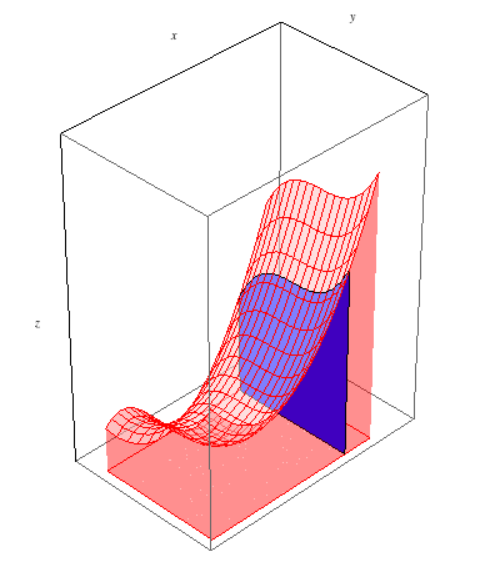
\includegraphics[width=10cm]{FubiniTonelli}
\end{figure}

In particular, it maps $x$ the measure of that slice, so we get a new function which at every slice captures the effect
of the $X$ component. After that, we integrate the function to get the effect from the $Y$ component. 

Furthermore, it will turn out that we can measure the slices with respect to $X$, or with respect to $Y$, and get the
same result, hence the second statement of this theorem! After proving the theorem, we'll go over why the assumption in
the statement of the theorem are important.


\begin{Proof}
	The way we will prove it is by taking advantage that rectangles already satisfy the property of the theorem, and since
	rectangles are a generating set for $\EM\otimes \EN$, we will be able to extend this result any measurable set. 

	We'll first prove it for when $\mu$ and $\nu$ are finite, and then generalize for when they are $\sigma$-finite. The
	way we'll do it is by starting with a subset of $\EM\otimes \EN$ for which we know the conclusion holds, and then
	generalize the result using the MCT and DCT. 


	Let $\CC$ be the subset of $\EM\otimes\EN$ for which the result of the theorem is true, that is, the two maps are
	measurable and we can integrate one way or another. Then if $A \in \EM$ and $B \in \EM$, we have that $A\times B \in
	\CC$. To see this, first compute the values $\nu(E_x)$ and $\mu(E^y)$:
	\[
		\nu(E_x) = \chi_A(x)\nu(B) \qquad \mu(E^y) = \mu(A)\chi_B(y)
	\]
	Then the functions is clearly measurable, being a bump function, and:
	\[
		\int \nu(E_x)d\mu = \int \chi_A(x)\nu(B)d\mu = \mu(A)\nu(B) = \int mu(A)\chi_B(y)d\nu = \int \mu(E^y)d\nu
	\]
	Showing the two integrals are equivalent, and since $(\mu\times \nu)(A\times B) = \mu(A)\nu(B)$, all equality hold,
	and so $E = A\times B \in \CC$. By additivity of the integral, it follows that all finite disjoint
	unions of rectangles are also in $\CC$. Thus, by lemma~\ref{lm:monotoneClassLem}, it suffices to show that $\CC$ is
	a monotone class, for then it is a $\sigma$-algebra containing the generating set of $\EM\otimes\EN$, meaning $\CC
	\supseteq \EM\otimes \EN$, and so all measurable sets can be broken down in this way. 

	First, let $\{E_n\}_{n=1}^\infty \sse \CC$ be an increasing subset and let $E =\bigcup_n^\infty E_n$. We want to
	show that $E \in \CC$. Then since $E_n \in \CC$ for all $n \in \N$, the sequence of $y$-section functions $f_n$,
	$f_n(y) = \mu((E_n)^y)$ are measurable and increase pointwise to $f(y) = \mu(E^y)$. By
	corrollary~\ref{co:measFuncPointLimt}, $f$ is measurable. Thus, we can find the value of $\int \mu(E^y)d\nu$ by
	applying the Monotone Convergence Theorem:
	\begin{align*}
		\int \mu(E^y)d\nu &= \int \lim_{n \rw \infty} \mu((E_n)^y)\nu\\
						  &= \lim_{n \rw \infty} \int \mu((E_n)^y)\nu\\
						  &= \lim_{n \rw \infty} (\mu\times \nu)(E_n) &E_n \in \CC\\
						  &= (\mu\times\nu)(E) & \cup_i E_i = E
	\end{align*}
	Doing the same trick, we can see that:
	\[
		\int \nu(E_x)d\mu = (\mu\times\nu)(E)
	\]
	which combined together shows us that:
	\[
		\int \mu(E^y)d\nu = \int \nu(E_x)d\mu = (\mu\times\nu)(E)
	\]
	and so $E \in \CC$. 

	Next, let $\{E_n\}_{n=1}^\infty \sse \CC$ be a decreasing subset and let $\bigcap_n E_n = E$. Then sine $E_1 \in
	\CC$, the function $f_1$, $f_1(y) = \mu((E_1)^y)$ is measurable. In fact, it's in $L^1$, since:
	\[
		\mu((E_1)^Y) \le \mu(X) < \infty \qquad \nu(Y) < \infty
	\]
	and so the resulting integral must have finite measure. Furthermore, this function will dominate the sequence of
	functions $f_n$, and so we can apply the Dominated Convergence Theorem to do the same limit trick we have just done
	and conclude that $E \in \CC$. Therefore, $\CC$ is a monotone class, hence a $\sigma$-algebra containing the
	generating set of $\EM\otimes\EN$, and the result is true for all measurable sets. 

	Now, suppose that $\mu$ and $\nu$ are $\sigma$-finite. Then we can write $X\times Y$ to be the union of an
	increasing sequence of rectangles $\{X_i\times Y_i\}$ of finite measure. Thus, for any $E \in \EM\otimes \EN$, take
	$E\cap (X_i\times Y_i)$, then this set now has finite measure, and so what we have just proved applies giving us:
	\[
		(\mu\times\nu(E\cap (X_i\times Y_i)) = \int \chi_{X_i}(x)\nu(E_x\cap Y_i)d\mu = \int \mu(E^y\cap
		X_i)\chi_{Y_i}(y)d\nu
	\]
	and so, a final application of the Monotone Convergence Theorem gives us our desired result
\end{Proof}

The hypothesis that $\mu\times \nu$ is $\sigma$-finite is necessary. Without it (see exercise 46 in Folland).

Notice that the functions within the integral are in fact the values of characteristic functions! Hence by the linearity
of the integral, we have the result for simple functions. Thus, with the statement proven for simple functions on
$\EM\otimes\EN$, we move on to proving it for integrable functions in general:

\begin{thm}{Fubini-Tonelli Theorem}{fubiniTonelliThm}
	Let $(X, \EM, \mu)$ and $(N, \EN, \nu)$ be $\sigma$-finite measures. Then:
	\begin{enumerate}
		\item (Tonelli) If $f \in L^+(X\times Y)$, then the functions $g(x) = \int f_xd\nu$ and $h(y) \int f^yd\mu$ are
			in $L^+(X)$ and $L^+(Y)$ respectively, and 
			\[
				\int \left[\int f(x,y)d\nu(y)\right]d\mu(x) = \int f(x,y)d(\mu\times \nu) = \int\left[\int
				f(x,y)d\mu(x)\right]\nu(y)
			\]
		\item (Fubinni) If $f \in L^1(\mu\times \nu)$, then $f_x \in L^1(\nu)$ for a.e. $x \in X$ and $f^y \in L^1(\mu)$
			for a.e. $y \in Y$. Furthermore, the a.e. defined function $g(x) = \int f_xd\nu$ and $h(x) = \int f^yd\mu$
	\end{enumerate}
	The resulting integral is called the \emph{iterated integral}
\end{thm}


\begin{Proof}
	\begin{enumerate}
		\item This essentially comes down to using MCT and the standard representation of measurable functions. By
			theorem~\ref{th:fubiniTonneliBuildUp}, we have the simple functions satisfy the theorem. To extend it to
			integrable functions, take $f \in L^+(X\times Y)$, and let $\{f_n\}$ be some simple representation for it,
			that is, a sequence of simple functions converging upwards to $f$. From $\{f_n\}$, we have a corresponding
			$\{g_n\}$ and $\{h_n\}$ converging upwards to $g$ and $h$: $g_n =$ . By theorem~\ref{th:fubiniTonneliBuildUp},
			these functions are measurable, and so $h$ and $g$ are measurable. With this, we can put together all our
			information to form the following chain of equalities:
			\begin{align*}
				\int \left[\int f_x\,d\nu\right]\,d\mu =\int gd\mu &= \int \lim g_n\,d\mu\\
						   &= \lim\int g_n\,d\mu\\
						   &= \lim \int f_n\, d(\mu\times \nu) & \text{theorem ~\ref{th:fubiniTonneliBuildUp}}\\
						   &= \int f\,d(\mu\times\nu) & \text{MCT}\\
						   &= \lim \int f_n\, d(\mu\times \nu)\\
						   &= \lim\int h_n\,d\nu & \text{theorem ~\ref{th:fubiniTonneliBuildUp}}\\
				\int \left[\int f^y\,d\mu\right]\,d\nu =\int hd\nu &= \int \lim h_n\,d\nu 
			\end{align*}
			Thus establishing the equality of Tonelli's Theorem. Furthermore, since $\int f\,d(\mu\times \nu) <\infty$,
			then $g < \infty$ a.e. and $h < \infty$ a.e., so $\int f_x < \infty$ and $\int f^y < \infty$, and therefore
			$f_x \in L^1(\nu)$ and $f^y \in L^1(\mu)$, which some of the preliminary results for Fubini's Theorem.
		\item Let $f \in L^1(\mu\times \nu)$, so $f^+ \in L^+(\mu\times \nu)$ and $f^- \in L^+(\mu\times \nu)$ (or $\Re
			f$ and $\sgn f$). Thus, the result applies to each component function, and so by linearity applies to $f$
	\end{enumerate}
\end{Proof}

Often, the parenthesis are dropped, and we combine the integrals into a double integral:
\[
	\int \left[\int f(x,y)\,d\mu(x)\right]d\nu(y) = \int\int f(x,y)\,d\mu(x)\,d\nu(y) = \int\int f\, d\mu\,d\nu
\]

Also, you might wonder if instead of assuming $f \in L^+(X\times Y)$ or $f\in L^1(X\times Y)$, we can assume that each
$f_x \in L^+(\nu), f^y \in L^+(\mu)$ ($L^1$ respectively) and that the iterated integrals $\int \int f\,d\mu\,d\nu$ and
$\int \int f\,d\nu\,d\mu$ existed, then $f \in L^+(X\times Y)$ ($L^1$ respectively), that is, is the converse true? The
answer is actually no:

\begin{example}{converse not true}{fubiniConverseCounterEx}
	exercise 48
\end{example}

One practical application of Fubini-Tonelli's Theorem is to solve integrals by integrating over the simpler variable
first. Usually, one first uses Tonelli's theorme to evaluate the integral $\int f\,d(\mu\times \nu)$ as an iterated
integral $\int\int f\,d\mu\,d\nu$ and show that the result is finite, at which point Fubini's Theorem can be invoked to
get $\int\int f\,d\mu\,d\nu =\int\int f\,d\nu\,d\mu$. 

To close off the discussion on product measures, notice that if $\mu$ and $\nu$ are complete measure, $\mu\times\nu$ is
almost never a complete measure. Let $(X, \EM, \mu)$ and $(Y, \EN, \nu)$ be measure spaces, take $A \in \EM$ is
a non-empty set with $\mu(A) = 0$, and suppose $\EN \ne P(Y)$ (For example, choose $(\R, \EL, m)$ for both measure
sapces). If $E \in P(Y)\setminus \EN$, then $A\times E \notin \EM\times \EN$ since not all slices of $A\times E$ (in
particular, the slice $E$) are in the respective measure spaces (proposition~\ref{pr:sectionsMeas}). However, $A\times
E \sse A\times Y$, and $(\mu\times\nu)(A\times Y) = 0$ (since the measure is finite, any out-measure is equal to the
usual outer-measure on these sets, which is $\mu(A)\nu(Y)  = 0\cdot n = 0$, since we take on the convention that $0\cdot
\infty = 0$). Thus, $\mu\times \nu$ is not complete. If we want, we can apply theorem~\ref{th:measureCompleting} to
complete the measure, howver we can no longer directly apply Fubini-Tonelli's Theorem. (Put Why Here!). We thus have to
slightly amend Fubini-Tonelli's theorem for the completion:

\begin{thm}{Fubini-Tonelli's Theorem for Complete Measures}{FubiniTonelliForCompelte}
	Let $(X, \EM, \mu)$ and $(Y, \EN, \nu)$ be complete $\sigma$-finite measures and let $(X\times Y, \EL, \lambda)$ be
	the completion of $(X\times Y, \EM\otimes \EN, \mu\times \nu)$. If $f$ is $\EL$-measurable is either:
	\begin{enumerate}
		\item non-negative, that is $f \ge 0$
		\item $f \in L^1(\lambda)$
	\end{enumerate}
	Then $f_x$ is $\EN$-measurable for a.e. $x$ and $f^y$ is $\EM$-measurable for a.e. y, and if (2) applies as well,
	then $f_x$ and $f^y$ are integrable for a.e. $x$ and $y$. Furthermore, $x \mapsto \int f_x\,d\nu$ and $y \mapsto
	\int f^y\,d\mu$ are measurable (and in the case of (2), also integrable) and
	\[
		\int f\,d\lambda = \int\int f(x,y)\,d\mu(x)\,d\nu(y) = \int\int f(x,y)\,d\nu(y)\,d\mu(x)
	\]
\end{thm}

\begin{Proof}
	homework! Uses Fubini-Tonelli.
\end{Proof}

\section{The n-dimensional Lebesgue Integral}

In this section, we focus on $\R^n = \R\times \R\times \cdots \times \R$ with the completed product measure $m\times
m\times \cdots \times m = m^n$ on $\EL\otimes \EL\otimes \cdots\otimes \EL = \EL^n$. The domain $\EL^n$ of $m^n$ is
called the set of \emph{Lebesgue measurable sets in $\R^n$}: $(\R^n, \EL^n, m^n)$ (sometimes, we will restrict $m^n$ to have domain
$(\BB_\R)^n = \BB_{\R^n}$). If it is unambiguous, we will usually write $(\R^n, \EL^n, m)$, dropping the power on the
$m$, and for the $n = 1$ case, we will often write $\int f(x)\,dx := \int f\,dm$. 

The following 3 theorems are simply generalizations of previous properties of the Lebesgue measure. In the following, let $E
= \prod_{i=1}^n E_i$ where $E_i \sse \R$. We will call each $E_i$ the \emph{sides} of $E$

\begin{thm}{Simplifying outer-measure}{simplifyingLebegueMeasureRn}
	Suppose $E \in \EL^n$
	\begin{enumerate}
		\item $m(E) = \inf\set{m(U)}{E \supseteq U,\ \text{$U$ is open}} = \sup\set{m(K)}{K \sse E,\ \text{$K$ is compact}}$
		\item $E = A_1\cup N_1 = A_2\setminus N_2$ where $A_1 \in F_\sigma$, $A_2 \in G_\delta$, and $m(N_1) = m(N_2)
			= 0$
		\item If $m(E) < \infty$, for all $\epsilon > 0$, there is a finite disjoint collection of rectangles
			$\{R_i\}_{i=1}^n$ whose sides are intervals such that $m(E\Delta \cup_i^n R_i) < \epsilon$
	\end{enumerate}
\end{thm}

\begin{Proof}
	p. 70 in folland
\end{Proof}

\begin{thm}{completeness of $L^1(m)$}{completenessofL1InRn}
	Let $f \in L^1(m)$ and let $\epsilon > 0$. Then there exists a simple function $\phi = \sum_{i=1}^n a_i\chi_R$ where
	each $R_i$ is a product of intervals such that 
	\[
		\int |f-\phi| < \epsilon
	\]
	and there is a continuous function that vanishes outside a bounded set such that 
	\[
		\int |f-g| < \epsilon
	\]
\end{thm}

\begin{Proof}
	Just like in theorem~\ref{th:simpleFuncDenseL1}, approximate $f$ by a simple function, then apply
	proposition~\ref{th:simplifyingLebegueMeasureRn}(3) to approximate $\phi$ appropriately. Finally, approximate $\phi$
	by continuous functions by applying the natural generalization of the argument in theorem~\ref{th:simpleFuncDenseL1}
\end{Proof}

\begin{thm}{Translation Invariance in $\R^n$}{translationInvarianceRn}
	Let $(\R^n, \EL^n, m)$ be a measure space. Then $m$ is translation invariant, that is, for any $a \in \R^n$, if we
	define $\tau_a: \R^n \rw \R^n$, $\tau_a(x) = a+x$, then
	\begin{enumerate}
		\item If $E \in \EL^n$, then $\tau_a(E) \in \EL^n$ and $m(E) = m(\tau_a(E))$
		\item If $f: \R^n \rw \C$ is Lebesgue measurable, then so is $f\circ \tau_a$. Furthermore, if either $f \ge 0$
			or $f \in L^1(m)$, then $\int (f\circ \tau_a)\,dm = \int f\,dm$
	\end{enumerate}
\end{thm}

Notice that we did not mention scaling. This is because scaling is not abstracted to linear transformations which
requires more work to show how the scaling of a linear transformation affects the value, and so we will prove that later
in this section.

\begin{Proof}
	Folland p.71
\end{Proof}

(here, some on cube approximation and Jordan content)

I'll for now simply state the effect of linear transformations and come back to this:

\begin{thm}{Linear Transformation on Integrability}{intgbleAndLinTrans}
	Suppose $T \in GL_n(\R$). Then:
	\begin{enumerate}
		\item If $f$ is a Lebesgue measurable function on $\R^n$, so is $f\circ T$. If $f \ge 0$ or $f \in L^1(m)$,
			then:
			\[
				\int f\,dm = |\det(T)|\int f\circ T\,dm
			\]
		\item If $E \in \EL^n$, then so is $T(E)$, and $m(T(E)) = |\det(T)|m(E)$
	\end{enumerate}
\end{thm}


\begin{Proof}
	here
\end{Proof}

There is also the statement on how diffeomorphisms affect the integral. 



\chapter{Signed Measure and Differentiation}

here


\chapter[Lp sapce]{$L^p$ space}

here

\section{Basics}

So far, we have limited our attention to measurable functions $f$ such that $\int |f| < \infty$ and have labelled them
$L^1$. Often, what we are looking are function that in fact converge \emph{faster}, that is, that
\[
	\int |f|^p < \infty
\]
for some $p \ge 1$, including $\infty$ (which we will define shortly). We'll let $L^p$ be the equivalence class of the set of functions such that
$|f|^p$ is integrable. Lots of definition require that $f$ shrink at a certain speed in order for them to be
well-defined (Fourier series being the canonical example, see ref:HERE), which is why we are analysing this space. With this added restriction, it becomes harder
to prove certain properties of $L^p$ such as whether $L^p$ is a vector-space or is complete. Thus, what we will do here
by establishing the basics is showing that $L^p$ is indeed a vector space, and in fact a complete vector space (i.e.
a Banach space), and go over some relations between $L^p$ spaces. 


We will start by defining $L^p$ 

\begin{defn}{$L^p$}{lp}
	Let $f$ be measurable. Define the ``\emph{$p$-norm}'' to be:
	\[
		\left\| f\right\|_p = \left[\int |f|^p\, d\mu\right]^{1/p}
	\]
	Note that we have yet to prove it's a norm. From this norm, define:
	\[
		L^p(X, \EM, \mu) := \set{f: X \rw \C}{\text{ $f$ is measurable and $\left\| f\right\|_p < \infty$}}
	\]
\end{defn}

As with $L^1$, we often abbreviate to $L^p(\mu)$, $L^p(X)$, or just $L^p$. Just like $L^1$, two functions will be equal
in $L^p$ (i.e. belong in the same equivalence class) if they are equal almost everywhere. Furthermore, we claimed that
$\left\| \cdot \right\|_p$ is a norm. That $\|f \|_p = 0$ if and only if $f = 0$ a.e. comes almost immediately, since
\[
\left(\int |f|^p\right)^{1/p} = 0 \quad \text{ iff }\quad \int |f|^p = 0 \quad\text{ iff }\quad \int
|f| = 0 \quad\text{ iff } \quad f = 0 \text{ a.e.}
\]
For $\left\|cf\right\|_p = |c|\left\| f\right\|_p$, we take advantage of our normalisation:
\[
	\left\| cf\right\|_p = \left(\int |cf|^p\right)^{1/p} = \left(\int |c|^p|f|^p\right)^{1/p}
	= \left(|c|^p\right)^{1/p}\left(\int |f|^p\right)^{1/p} = |c|\left\|f\right\|_p
\]
However, the triangle inequality is not so trivial. We will in fact take good part of this section to show that the
triangle inequality is satisfied. For now, we take a moment to explore an example of an $L^p$ space to gain an
intuition:

\begin{example}{$L^p$ and counting measure}{countingMeasEx}
	\begin{enumerate}
		\item Let $f: [0, \infty) \rw \R$ $f(x) = \frac{1}{x^{1/p}}$. Then $f \in L^q$ for $q > p$. This comes down to the fact that:
			\[
				x > x^{1/p}\ \LRw\ \frac{1}{x} < \frac{1}{x^{1/p}}
			\]
			and by the fact that $\int\left|\frac{1}{x^n}\right| < \infty$ if $n > 1$. We have therefore found a class
			of functions that fits into all possible $p \in [1, \infty)$. In fact, we can find functions that fit into
			any connected subinterval of $[1, \infty)$! Take 
			\[
				\text{Here, q4b of hw}
			\]
			So if $f \in L^p$, it does not imply that $f \in L^q$ for $p > q$ or $p < q$! Later on, we will show some of
			the possible relations between $L^p$ spaces. 
		\item A particular case that will be common for analyzing sequences is when $\mu$ is the counting measure on $A$.
			In that case, we usually denote $L^p(\mu)$ by $l^p(A)$. If $A = \N$, we often simply abbreviate notation to $l^p$.
			If we write $f: \N \rw \R,\ f(k) = a_k$, then the sequence $f$ (i.e. $\{a_k\}$ is in $l^p$ if:
			\[
				\sum_{k=1}^\infty |a_k|^p < \infty
			\]
			Thus, $L^1$ is the set of convergence series. 
	\end{enumerate}
\end{example}

Notice that we are ``normalizing'' each integral by a factor of $1/p$. This normalization is done to make sure that the
constant can be brought out of the norm. It might seem tempted to say that:
\[
	\left(\int |f|^p\right)^{1/p} \text{ ``$=$'' } \int |f|
\]
However, this is most certainly not true (simply take $x$ and see for yourself). As mentioned before, this makes it
non-trivial to show that $\left\| \cdot\right\|_p$ is a norm on $L^p$. However, it is easy to see that $L^p$ is
a vector-space. If $f,g \in L^p$, then:
\[
	|f+g|^p \le [2\max(|f|, |g|)]^p \le 2^p(|f|^p + |g|^p)
\]
which is finite by assumption, and so $f+g \in L^p$. It is also immediate that $cf \in L^p$. Thus, we may freely add and
multiply by $L^p$ functions without worrying about leaving $L^p$. Because of this, it makes it meaningful to ask whether
\[
	\left\| f_1 +f_2\right\|_p \le \left\| f_1\right\|_p + \left\|f_2\right\|_p
\]

What we will now do is show that $\left\| \cdot \right\|_p$ is does indeed satisfy the triangle inequality or $p \ge 1$.
If $p < 1$, then the triangle inequality in fact fails. 

\begin{example}{$p < 1$ then no Triangle Inequality}{plessthan1Case}
	Take $a, b > 0$ and $0 < p < 1$. Then we have that:
	\[
		t^{p-1} > (a + t)^{p-1}
	\]
	Integrating both sides from $0$ to $b$, we get:
	\begin{align*}
		\int_0^bt^{p-1} &> \int_0^b (a + t)^{p-1}\\
		\frac{b^p}{p} &> \frac{(a+b)^p}{p}\\
		b^p &> (a+b)^p\\
		a^p + b^p &> (a+b)^p\\
	\end{align*}
	Thus, if $E$ and $F$ are disjoint union with positive finite measures in $X$ such that $\mu(E)^{1/p} = a$ and
	$\mu(E)^{1/p} = b$, taking advantage of the fact that $\chi_E\chi_F = 0$ (i.e. the zero function) since $E\cap
	F = \emptyset$, then:
	\[
		\left\| \chi_E + \chi_F\right\|_p = (a^p + b^p)^{1/p} > a+b = \left\| \chi_E\right\|_p + \left\| \chi_F\right\|_p
	\]
	Giving us that the triangle inequality does not hold. 
\end{example}

Thus, we stick to showing the case where $p \ge 1$ First, we will state a simple inequality fact similar Jensen's
inequality. This is in fact the key idea behind the entire proof:
\begin{lem}{Young's Inequality}{YoungInequality}
	If $a,b \ge 0$ and $0 < \lambda < 1$, then:
	\[
		a^\lambda b^{1-\lambda} \le \lambda a + (1-\lambda)b
	\]
	with equality if and only if $a = b$. In particular, notice that if $\frac{1}{p} + \frac{1}{q} = 1$, then if
	$\lambda = p^{-1}$, $(1-\lambda) = q^{-1}$ and so:
	\[
		a^{p^{-1}} b^{q^{-1}} \le p^{-1} a + q^{-1}b
	\]
\end{lem}

\begin{Proof}
	This proof is trying to capture what this image is doing in formal language:
	\begin{center}
		\url{https://www.desmos.com/calculator/jdznjzqcju}
	\end{center}

	If $a= b$, equality clearly holds. If $a = 0$ or $b = 0$, inequality clearly holds. If $a,b \ne 0$, then dividing by $b$ and letting $t = a/b$, we
	get
	\begin{equation}\label{eq:YoungIneq}
		a^\lambda b^{-\lambda} \le \lambda(a/b) + (1-\lambda) \quad \LRw\quad t^\lambda \le \lambda t + (1-\lambda)\quad
		\LRw\quad t^\lambda - \lambda t \le (1-\lambda)
	\end{equation}
	From here, we use some calculus: we see that $t^\lambda - \lambda t$ is strictly
	increasing for $0 < t < 1$ (since $a,b \ge 0$, $t \ge 0$) and strictly decreasing for $t > 1$, so the maximal value occurs at $t = 1$, and in fact we
	get that the maximal value is $1 - \lambda$:
	\[
		1^\lambda - \lambda 1 = 1- \lambda \le 1- \lambda
	\]
	and so the inequalities in equation~(\ref{eq:YoungIneq}) hold! Equality happens when $t = a/b = 1$ which implies $a=
	b$, completing the proof. 
\end{Proof}

Usually, Young's inequality is stated as 
\[
	a^\alpha b^\beta \le \alpha a + \beta b \qquad 0 \le \alpha,\beta \le 1,\quad \alpha + \beta = 1
\]
which is exactly what we have, since if we fix some $\alpha$, then it must be that $\beta = 1-\alpha$. Another
formulation of Young's inequality is:
\[
	ab \le \frac{a^p}{p} + \frac{b^q}{q}
\]
with $p^{-1} + q^{-1} = 1$. This proof is a ``Jensen equality'' like proof that more clearly shows the role of concavity and so I'll dedicate
a moment to prove this one too:
\begin{Proof}
	If $a = 0$ or $b =0$, the result is immediate, so assume $a,b > 0$. Then notice that since log is monotone:
	\[
		ab \le \frac{a^p}{p} + \frac{b^q}{q}\quad \LRw\quad \log(ab) \le \log\left(\frac{a^p}{p} + \frac{b^q}{q}\right)
	\]
	which is great, since we know log is concave and so Jensen's inequality applies. Since $p^{-1} + q^{-1} = 1$, we get
	$t = 1/p$ and $(1-t) = 1/q$, and so by Jensen's inequality:
	\[
		\log(ta^p + (1-t)\b^q) \ge t\log(a^p) + (1-t)\log(b^q) = \frac{p}{p}\log(a) + \frac{q}{q}\log(b)
		= \log(ab)
	\]
	completing the proof. 
\end{Proof}

The second interpretation of $p^{-1} + q^{-1} = 1$ in Young's inequality is a nice way to write the straight line (or
sub-straight line) equation without the $1-\lambda$ term, but just two numbers. It furthermore let's us relate two
numbers that can be much larger. For example, if I choose $p
= 100$, then it must be that $q = 100/99$ so that 
\[
	p^{-1} + q^{-1} = 1/100 + 99/100 = 1
\]
which, if we consider $p$ and $q$ to be the exponents associated to $L^p$ and $L^q$, we see that this gives us a way to
relate different $L^p$ space! 

To see this, we use this convexity property given by Young's inequality in the ``build-up'' lemma towards the triangle
inequality. This lemma is important later on in functional analysis, but for our purposes is important for the triangle
inequality:

\begin{thm}{H\"older's Inequality}{holderInequality}
	Let $1 \le p,q \le \infty$ satisfy:
	\[
		\frac{1}{p} + \frac{1}{q} = 1
	\]
	or equivalently $q = p/(p-1)$, where we will interpret $\frac{1}{\infty}$ as $0$. Then if $f$ and $g$ are measurable
	functions on $X$ then:
	\[
		\left\| fg\right\|_1 \le \left\| f\right\|_p \left\|g\right\|_q
	\]
	In particular, if $f \in L^p$ and $g \in L^q$ then $fg \in L^1$. Equality holds if and only if $\alpha|f|^p
	= \beta|g|^q$ a.e. for some constants $\alpha, \beta$ with $\alpha\beta \ne 0$
\end{thm}
Notice that when $p = q = 2$ (if $p = 2$, it must be that $q = 2$ to satisfy the equation), then this inequality is
called the \emph{Cauchy-Schwartz inequality}. Notice too that this is the only time when $p = q$; this will become
important when we analyze the $p = 2$ case later. 

(I also want to include a quick word on Cauchy-Schwartz inequality since I didn't know how important it is: (commented))
%https://en.wikipedia.org/wiki/Cauchy%E2%80%93Schwarz_inequality

\begin{Proof}
	If $\left\| f\right\|_p = 0$ or $\left\| g\right\|_p =  0$, then $f = 0$ or $g= 0$ a.e., and so equality holds.
	Similarly if $\left\| f\right\|_p = \infty$ or $\left\| g\right\|_p = \infty$, inequality immediately holds. Furthermore, notice that if we find
	a particular $f$ and $g$ for which the result holds, then the result holds for $af$ and $bg$ since
	\[
		|ab|\left\|fg\right\|_1 \le |ab|\left\|f\right\|_p\left\|g\right\|_q
	\]
	So, it suffices to show the result when $\left\|f\right\|_p = \left\| g\right\|_q = 1$, and equality holds of $|f|^p
	= |g|^q = 1$. To this end, we use the previous lemma and set $a = |f(x)|^p$ and $b = |g(x)|^q$ and $\lambda
	= p^{-1}$ (so that $1-\lambda = 1-p^{-1} = q^{-1}$). Then by the previous lemma we have:
	\begin{equation}\label{eq:holdInequality}
		|f(x)|^{p\cdot p^{-1}}|g(x)|^{q\cdot q^{-1}} \le p^{-1}|f(x)|^p + q^{-1}|g(x)|^q\quad \LRw\quad |f(x)g(x)| \le p^{-1}|f(x)|^p + q^{-1}|g(x)|^q
	\end{equation}
	Now, integrating both sides, we get:
	\[
		\left\| fg\right\|_1 \le p^{-1}\int |f|^p + q^{-1}\int |f|^q = p^{-1} + q^{-1} = 1 = \left\| f\right\|_p \left\|
		g\right\|_q
	\]
	where equality holds when equality holds in equation (\ref{eq:holdInequality}) a.e., which holds only when $|f|^p
	= |g|^q$ a.e., as we sought to show
\end{Proof}

When $p$ and $q$ satisfy the equality in the equation, we call them \emph{conjugate exponents}. As mentioned before, the
conjugate exponents is simply another way or writing the equation of a straight line to apply Young's inequality. From
this, we can take advantage of this convexity property yet again to prove the triangle inequality of $\left\| \cdot
\right\|_p$, which has a different name since for the special case of the $p$-norm due to the fact it is used on other
places and needs to be referenced:

\begin{thm}{Minkowski's Inequality}{minkowskiInequality}
	If $1 \le p < \infty$ and $f,g \in L^p$. Then:
	\[
		\left\|f+g\right\|_p \le \left\|f\right\|_p+\left\|g\right\|_p
	\]
\end{thm}

Before proceeding with the proof, a quick word a common notation convention:
\[
	\left\| f\right\|_p^p = \left(\int |f|^p\right)^{p/p} = \int |f|^p
\]
In as sense, this is not a convention, but just $\left(\left\|f\right\|_p\right)^p$. However, I have gotten thrown off
by this notation, so I felt a remark was in order.

\begin{Proof}
	If $p = 1$, then the result immediately follows by the regular triangle inequality and linearity of the integral. If
	$f + g = 0$ a.e., then the result also follows, so assume that $f + g \ne 0$ a.e., which using the triangle
	inequality:
	\[
		|f+g|^p \le (|f| + |g|)|f+g|^{p-1} = |f||f+g|^{p-1} + |g||f+g|^{p-1}
	\]
	So, we will apply H\"older's inequality using the fact that $q = \frac{p}{p-1}$ and integrating:
	\begin{align*}
		\left\|f+g\right\|_p^p &= \int |f+g|^p d\mu\\
								  &= \int |f+g|\cdot |f+g|^{p-1}d\mu\\
								  &\le \int(|f|+|g|)|f+g|^{p-1}d\mu\\
								  &= \int |f||f+g|^{p-1}d\mu
								  + \int|g||f+g|^{p-1}d\mu\\
								  &= \left\| |f|(|f+g|^{p-1})\right\|_1 + \left\| |g|(|f+g|^{p-1})\right\|_1\\
								  &\le \left\| |f|\right\|_p\left\|f+g\right\|_q^{p-1}
								  + \left\|g\right\|_p\left\|f+g\right\|_q^{p-1}
								  & \text{H\"older's Inequality}\\
								  &=
								  \left(\left(\int|f|^p d\mu\right)^{\frac{1}{p}}
									  + \left(\int|g|^p d\mu\right)^{\frac{1}{p}}\right)\left(\int
								  |f+g|^{(p-1)\left(\frac{p}{p-1}\right)}d\mu\right)^{\frac{p-1}{p}}
								  &\text{recall }q = \frac{p}{p-1}\\
								  &=
								  \left(\left(\int|f|^p d\mu\right)^{\frac{1}{p}}
									  + \left(\int|g|^p d\mu\right)^{\frac{1}{p}}\right)\left(\int
								  |f+g|^{p}d\mu\right)^{\frac{p-1}{p}}\\
								  &= (\left\|f\right\|_p + \left\|g\right\|_p)
								  \frac{\left\| |f+g|^p\right\|_p}{\left\|
								  f+g\right\|_p}
	\end{align*}
	Thus, multiplying both sides by $\frac{\left\| |f+g|^p\right\|_p}{\left\| f+g\right\|_p}$, we get
	\[
		\left\| f+g\right\|_p \le \left\|f\right\|_p + \left\|g\right\|_p
	\]
	As we sought to show
\end{Proof}


Thus, we get that $\left\| \cdot \right\|_p$ is indeed a norm! Thus $L^p$ is a normed vector space. In fact, just like
$L^1$, it is a complete normed vector space, i.e., a Banach space. We first prove a lemma to simply our task. To
understand the lemma, notice that every norm defines a metric:
\[
	\rho(x,y) = \left\| x-y\right\|
\]
and so defines a topology, in particular a normal space, that has the notion of sequences well-defined. Next, if
$\{x_n\}$ is a sequence in $V$, it's series is said to converge if there exists an $x \in V$ such that
$\sum_{n=1}^\infty x_n = x$, and is said to be absolutely convergence if $\sum_{n=1}^\infty \left\| x_n\right\|
< \infty$

\begin{lem}{Cauchy and Absolute Convegence}{cauchAndAbsConv}
	Let $V$ be a normed vector space. Then $V$ is complete if and only if every absolutely convergent series in $V$
	converges. 
\end{lem}

\begin{Proof}
	Let's first say that $X$ is complete and that $\sum_{n=1}^\infty \left\| x\right\| < \infty$. To show it converges,
	we take advantage of complete and show there is a Cauchy sequence. In particular, let $S_n = \sum_{k=1}^n x_k$. Then
	since the series is absolutely convergent, there for all $n > m$, 
	\[
		\left\| S_n - S_m\right\| \le \sum_{m+1}^n \left\| x_k\right\| \rw 0 \quad\text{as $m,n \rw \infty$}
	\]
	so the sequence $\{S_n\}$ is Cauchy, and so converges. 

	Conversely, let's say an absolutely convergent series converges, and choose any Cauchy sequence $\{x_k\}$. Since
	it's a Cauchy sequence, choose a subsequence such that
	\[
		\left\| x_{k_{i+1}} - x_{k_i}\right\| < 2^{-i}
	\]
	Take $y_1 = x_{k_1}$ and $y_i = x_{i+1} - x_i$ for $i>1$ so that $\sum_{i=1}^n y_i = x_{k_n}$. Then notice that
	$\{y_i\}$ is in fact absolutely convergent:
	\[
		\sum_{i=1}^\infty \left\| y_i\right\| \le \left\| y_1\right\| + \sum_{i=1}^\infty 2^{-i} = \left\| y_1\right\|
		+ 1 < \infty
	\]
	So $\sum_{i=1}^\infty y_i = \lim x_{k_n}$ exists. Since the subsequence of every Cauchy sequence approaches the same
	``point'' (just like convergent sequences), we see that $\{x_n\}$ also converges to the same point, showing that
	Cauchy sequences are in fact convergent sequences, as we sought to show. 
\end{Proof}

\begin{thm}{$L^p$ is a Banach Space}{lPIsBanachSp}
	For $1 \le p < \infty$, $L^p$ is a complete normed vector-space, i.e., a Banach space. Moreover, if $f-n \rw f$ in
	$L^p$, then there exists a subsequence that converges pointwise to $f$ a.e.
\end{thm}

\begin{Proof}
	Let $1 \le p < \infty$. By the previous lemma, it suffices to show that every absolutely convergent series converges:
	\[
		\sum_{k=1}^\infty \left\| f\right\|_p = B < \infty \quad \Rw\quad \exists f \text{ s.t. } \sum_{k=1}^\infty f_k = f \in L^p
	\]
	Let $G_n = \sum_{k=1}^n |f_k|$ be the partial sums of the series and $G = \sum_{k=1}^\infty |f_k|$ be the series.
	Then by Minkowski's inequality, we get:
	\[
		\left\| G_n\right\|_p \le \sum_{k=1}^n \left\| f_k\right\|_p \le B \quad \forall n \in \N
	\]
	and so $\left\| G\right\|_p  = \left(\int |G|^p\right)^{1/p}< \infty$ and so $\left(\int |G|^p\right) < \infty$.
	Since $G_n \le G_{n+1}$, and $G_n: X \rw [0, \infty)$, by the Monotonce Convergence Theorem:
	\[
		\int \lim_{n \rw\infty} G_n^p = \lim_{n \rw \infty} \int G_n^p \le B^p < \infty
	\]
	and so $G \in L^p$. By proposition~\ref{pr:propIntbleFunc}, $G(x) < \infty$ a.e., so the series $\sum_{k=1}^\infty
	f_k$ converges a.e. If we let $F = \sum_{k=1}^\infty f_k$, we have that $|F| \le G$ a.e., and so $F \in L^p$. From
	this, we can see that:
	\[
		\left\|F - \sum_{k=1}^\infty f_k\right\|_p^p = \int \left| F - \sum_{k=1}^\infty f_k\right|^p \rw 0
	\]
	Thus, the series $\sum_{k=1}^\infty f$ converges (to $F$) in the $p$-norm, and so by lemma~\ref{lm:cauchAndAbsConv},
	$L^p$ is complete, as we sought to show. 



	This is the proof the prof was doing in class, but I got stuck so found a different proof (the above proof)
	(Commented it out for now)
	%We've already shown it's a normed vector-space, so it remains to show that for any sequence $\{f_n\} \sse L^p$ such
	%that $f_n \rw f$ that $f \in L^p$

	%Let $\{f_n\} \sse L^p$ be a cauchy-sequence. Choose a subsequence $\{f_{n_i}\}$ such that:
	%\[
	%	\left\| f - f_{n_i}\right\|_p < 2^{-i}
	%\]
	%Define the telescoping sum:
	%\[
	%	g_k(x) = \sum_{i=1}^k |f_{n_{i+1}}(x) - f_{n_i}(x)| \quad g(x) =\sum_{i=1}^\infty |f_{n_{i+1}}(x) - f_{n_i}(x)|
	%\]
	%Then by the triangle inequality (i.e. Minkowski's inequality), we get:
	%\[
	%	\left\| g_k\right\| \le \sum_{i=1}^k 2^{-i} \le 1 \qquad \forall k
	%\]
	%and so by how $g$ is defined, 
	%\[
	%	g_k^p \rw g^p \qquad \lim_{k \rw \inft} g_k^p(x) = g^p(x)
	%\]
	%that is, $g_k$ converges pointwise to $g$, and so $g_k^p$ ($g$ to the power of $p$) converges pointwise to $g^p$.
	%Thus, by Fatou's lemma, we get that:
	%\[
	%	\int g^p \le \liminf_{k \rw \infty} \int g_k^p \le 1 
	%\]
	%and since $g_k^p$ converges pointwise to $g^p$, it must be that:
	%\[
	%	\left\| g\right\|_p \le 1
	%\]
	%so $g(x) < \infty$ a.e., and so we can define the telescoping sum:
	%\[
	%	f_{n_1}(x) + \sum_{c=1}^\infty (f_{n_{i+1}}(x) - f_{n_{i}}(x))
	%\]
	%which converges absolutely a.e.; thus define
	%\[
	%	f(x) = f_{n_1}(x) + \sum_{c=1}^\infty (f_{n_{i+1}}(x) - f_{n_{i}}(x))
	%\]
	%This is a telescoping series, and moreover
	%\[
	%	\lim_{k \rw \infty} f_{n_k}(x) = f(x)
	%\]
	%point-wise a.e. I claim that:
	%\[
	%	\left\| f - f_{n_k}\right\|_p \rw 0
	%\]
\end{Proof}

This also finally showed that $L^1$ is a complete space under $\left\| \cdot \right\|$! Furthermore, we can now extend
theorem~\ref{th:simpleFuncDenseL1} to show that simple function are dense in every $L^p$!

\begin{thm}{Simple Functions Dense in $L^p$}{simpleFuncDenseLp}
	For $1 \le p < \infty$, the set of simple functions $f = \sum_{i=1}^n a_i \chi_{E_i}$ where $\mu(E_i) < \infty$ for
	all $i$ is dense in $L^p$
\end{thm}

\begin{Proof}
	First of all, the set of simple functions is in $L^p$ for every $1 \le p < \infty$. Next, choosing any $f \in L^p$,
	choose some standard representation $\{f_n\}$ where $f_n \rw f$ a.e. Then sine $|f_n| \le |f|$, we get that $|f_n|
	\in L^p$. Furthermore
	\[
		|f-f_n|^p \le |2f|^p = 2^p|f|^p \in L^1
	\]
	and so by the dominated convergence theorem, we get:
	\[
		\int |f - f_n|^p \rw 0 \quad \Rw\quad \left(\int |f - f_n|^p\right)^{1/p} = \left\| f - f_n\right\|_p \rw 0
	\]
	Moreover, if $f_n = \sum_{k=1}^\infty a_k\chi_{E_k}$ was a simple function where all $E_i$ are pairwise disjoint and
	$a_i$ are nonzero, it must be that $\mu(E_i) < \infty$ since
	\[
		\sum_{k=1}^\infty |a_k|^p\mu(E_k) = \int |f|^p < \infty
	\]
	completing the proof
\end{Proof}

\begin{figure}[H]
	\centering
	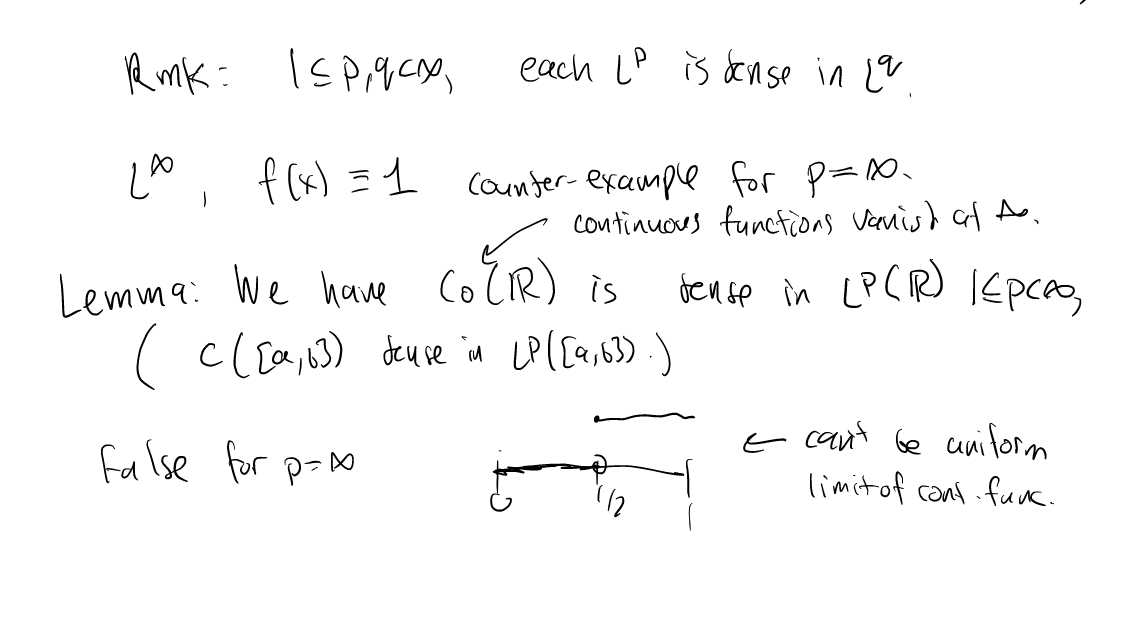
\includegraphics[width=10cm]{toInclude}
\end{figure}

So far, we have defined $L^p$ spaces where $0 < p < \infty$ and showed that for $1 \ge p < \infty$, $L^p$ is a Banach
space. However, if you take a look at a graph of $\left\| f\right\|_p$ as $p \rw \infty$, you'll find that there is
a striking pattern that comes back many times:

\begin{figure}[H]
	\centering
	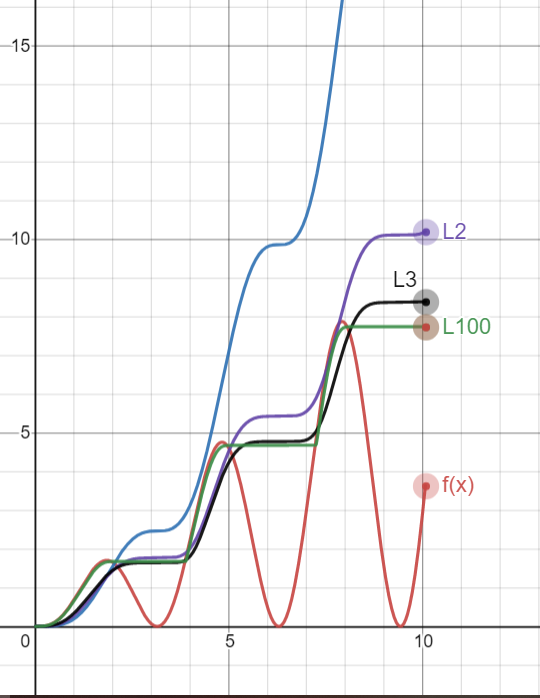
\includegraphics[width=10cm]{LInftyNorm}
\end{figure}
Notice that as $p \rw \infty$, the resulting $\|f\|_p$ value got closer to a max function. In fact, that is indeed the
case! We might be tempted to then say that $\|f\|_\infty = \sup f$. However, the problem with this is that we might have
a measure $0$ set that diverges, while the supremum of the rest of the function is attained by a value $k < \infty$.
The idea of $\sup f$ on all but a zero measure set will be called the \emph{essential supremum}, and all functions that
have a finite essential supremum will be denoted as $L^\infty$. In this way, $L^\infty$ is simply a natural extension of our definition of $L^p$:

\begin{defn}{$L^\infty$}{lInfty}
	Let $(X, \EM, \mu)$ be a measure space and let $f: X \rw [0, \infty]$ be a measurable function. Let 
	\[
		S = \set{r \in \R }{\mu(f^{-1}((r, \infty])) = 0}
	\]
	Then the \emph{essential supremum} of $f$, denoted $\left\| f\right\|_{\infty}$ or $\esssup f$ is :
	\[
		\left\| f\right\|_{\infty} := \begin{cases}
			\infty & \text{ if $S = \emptyset$}\\
			\inf S & \text{ if $S \ne \emptyset$}
		\end{cases}
	\]
	or, equivalently:
	\[
		\|f\|_\infty = \inf_{\substack{E \in \EM\\ \mu(X\setminus E) = 0}} \left(\sup_{x \in E} |f(x)|\right)
	\]
	If $f$ is a complex measurable, function, then $\left\| f\right\|_\infty = \left\| |f|\right\|_\infty$
\end{defn}

Essentially, $\| f\|_\infty$ is the least upper bound of $f$, ignoring measure zero sets worth of points.  Using this
definition, we can define $L^\infty$ to be the equivalence classes of functions $f$ such that $\left\| f\right\|_\infty
< \infty$. 

(Make this rigorous) Another quick way of visualizing these norms is by taking the set of all points $\R^2$ such that $\|(x,y)\|_p = 1$
A quick visual way of seeing the relation between $L^p$ and $L^\infty$ is as
follows: if we take $X = R^2$ and take $S_p =  \set{x \in \R^2}{\left\|x\right\|_p = 1}$,
we'd get

\begin{figure}[H]
	\centering
	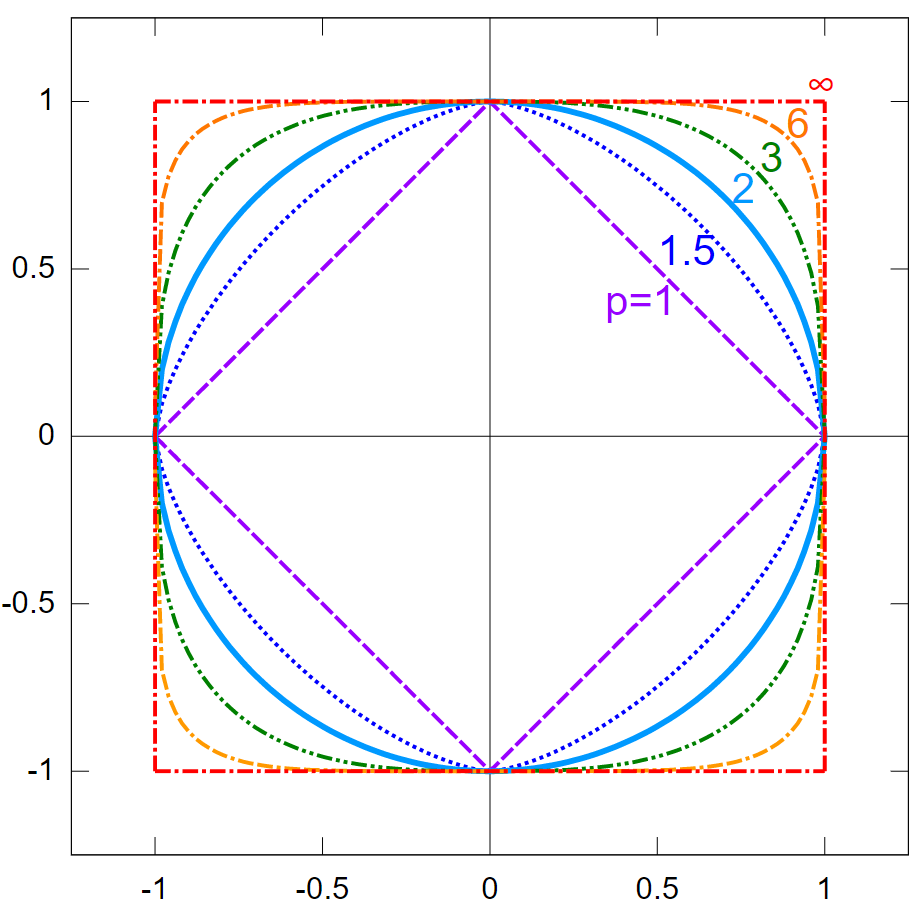
\includegraphics[width=10cm]{p-norm_example}
\end{figure}

(some remarks Folland does on p. 184)

\begin{prop}{Properties of $L^\infty$}{propLInfty}
	Let $(X, \EM, \mu)$ be a measure and $L^\infty$ the set of measurable function such that $\|f\|_\infty < \infty$.
	Then:
	\begin{enumerate}
		\item If $f,g$ are measurable functions on $X$, then 
			\[
				\left\| fg\right\|_1 \le \left\|f\right\|_1\left\|g\right\|_\infty
			\]
			If $f \in L^1$ and $g \in L^\infty$, then $\left\| fg\right\|_1 =
			\left\|f\right\|_1\left\|g\right\|_\infty$ if and only if $|g(x)| = \|g\|_\infty$ a.e. on the set where
			$f(x) \ne 0$
		\item $\left\|\cdot \right\|_\infty$ is a norm on $L^\infty$
		\item $\left\| f_n -f\right\|_\infty \rw 0$ if and only if there exists $E \in \EM$ such that $\mu(E^c) = 0$ and
			$f_n \rw f$ uniformally on $E$
		\item $L^\infty$ is a Banach space
		\item The simple functions are dense in $L^\infty$
	\end{enumerate}
\end{prop}

As a consequence of the well-definedness of $L^\infty$, $1^{-1} + \infty^{-1} = 1$ is indeed a well-defined notion
(since $\infty^{-1} = 1/\infty = 0$. Thus, $1$ and $\infty$ are conjugate exponents!
\begin{Proof}
	\begin{enumerate}
		\item We'll be using the $\|f\|_\infy = \inf_{\substack{E \in \EM\\ \mu(X\setminus E) = 0}}\left(\sup_{x \in E}
			|f(x)|\right)$ definition of the essential supremum to take advantage of the supremum within the definition.
			Our goal is to show that 
			\[
				\int |fg| = \|fg\|_1 \le \|f\|_1\|g\|_\infty
			\]
			First, we will limit our attention of $\int |fg|$ to some $E \in \EM$ such that $\mu(X\setminus E)
			= \mu(E^c) = 0$ (i.e., we are ignoring finite-measure points). Then:
			\[
				\int |fg| = \int_{E} |fg| + \int_{E^c} |fg| = \int_E |fg|
			\]
			Next, we take advantage the fact that we are working with an infimum to see that:
			\[
				\|f\|_\infty \le \sup_{x \in A} |f(x)| < \|f\|_\infty + \epsilon
			\]
			Therefore, we can take:
			\[
				\int_E |fg| \le \int_E |\sup_{x in E}|f(x)|\cdot g| = \int_E \left|\sup_{x \in E}|f(x)|\right|\cdot |g|
				= \left|\sup_{x \in E}|f(x)|\right|\int_E |g|
			\]
			where the last equality comes from the fact that the supremum is a constant. Finally, by the property of the
			infimum, we have:
			\[
				\left|\sup_{x \in E}|f(x)|\right|\int_E |g| \le (\|f\|_\infty + \epsilon)\int |g|
			\]
			Notice that this inequality does not depend on $\epsilon$, and so:
			\[
				\|fg\|_1 = \int_E |fg| \le  \|f\|_\infty\|g\|_1
			\]
			as we sought to show
	\end{enumerate}
\end{Proof}

\subsection[Relating Lp sapces]{Relating $L^p$ spaces}

In this section, we will show how we can relate $L^p$ spaces with each other. Fundamentally, the way we get any order
with $L^p$ spaces is through H\"older's inequality. We take full advantage of it in the following proofs. The end-goal
is to show that if $p < q < r$ where we allow $r = \infty$, then:
\[
	L^p \cap L^r \sse L^q \sse L^p + L^r
\]
which at first glance might seem strange since it feels like the relation should be $L^p \sse L^q$ for $p < q$ (or the
contravariant). However, as we saw in example~\ref{ex:countingMeasEx}, due to the varying types of growths a function
can have (in particular, it can shrink too slowly to have a finite measure, or it explodes at some point, or
a combination of both), the relationship is not so simple. We thus explore these relation's in this section. 


\begin{prop}{$L^p$ subset}{lpInclusion}
	Let $0 < p < q < r \le \infty$. Then
	\[
		L^q \sse L^p + L^r
	\]
	In particular, each $f \in L^q$ is the sum of a function in $L^p$ and a function in $L^q$
\end{prop}

\begin{Proof}
	very short. p.185
\end{Proof}

\begin{prop}{$L^p$ superset}{lpContainement}
	Let $0 < p < q < r \le \infty$. Then
	\[
		L^p \cap L^r \sse L^q
	\]
	In particular, if if we find that $f$ is bounded in growth from above and bellow by $p$ and $q$, $\|f\|_p < \infty$ and $\|f\|_r
	< \infty$, then $f$ is bounded in growth by $q$. 

\end{prop}

\begin{Proof}
	Let $\|f\|_r < \infty$ and $\|f\|_q < \infty$. We need to show that $\|f\|_p < \infty$. Notice that it is equivalent
	to show that $\|f\|_r^n < \infty$ and $\|f\|_q^m < \infty$ then $\|f\|_p^\ell < \infty$ for $n,m,\ell \in \R_{\ge 0}$ (since
	if it's finite, then all powers will be finite). We'll prove it in the case where $r = \infty$ and $r < \infty$. In
	the infinite case, we simply take advantage of bounding properties of the essential supremum, and in the other case
	we use H\"older's inequality. 

	 Starting with the $r = \infty$ case,
	notice that
	\[
		|f|^q  = |f|^{q-p+p} = |f|^q|f|^{q-p} \le \|f\|_\infty^{q-p}|f|^p
	\]
	and so, taking the integral and the $q$th root, we get:
	\begin{align*}
		\|f\|_q &= \left(\int |f|^q\right)^{1/q}\\
				&\le \left(\int \|f\|_\infty^{q-p}|f|^p\right)^{1/q}\\
				&= \|f\|_\infty^{\frac{q-p}{q}}\left(\int |f|^p\right)^{1/q}\\
				&=  \|f\|_\infty^{\frac{q-p}{q}}\left(\int |f|^p\right)^{p/pq}\\
				&= \|f\|_\infty^{1-\frac{p}{q}} \|f\|_p^{p/q} < \infty
	\end{align*}
	The fact that the last inequality is less than infinity comes from the that $\|f\|_p < \infty$ and $\|f\|_\infty
	< \infty$, so any power is less than infinity, and so $\|f\|_q < \infty$. Furthermore, notice that the sum of the
	power's is $1$; this fact will come back for another intuition of $\|f\|_\infty$. 
	%define the continuous function $\lambda \mapsto \frac{\lambda}{p}$. Since $1/q < 1/p$ and the function maps
	%connected intervals to connected intervals, there exists a $\lambda_0$ such that $\frac{\lambda_0}{p} = \frac{1}{q}$.
	%In fact, we can precisely determine $\lambda_0$ to be $\frac{p}{q}$. So:
	%\[
	%	\frac{(p/q)}{p} = 1/q \quad\LRw\quad \frac{q(p/q)}{p} = 1\quad\LRw\quad \frac{1}{\frac{p}{q(p/q)}}
	%	+ \frac{1}{\infty}
	%	= 1
	%\]
	%Thus, by H\"olders inequality, we get:
	%\[
	%	|f|^q = (|f|^{q-p}|f|^{q})
	%\[
	%	here
	%\]


	For the $r < \infty$ case the key is to find a way to integrate $p$ and $r$ using conjugate exponents. Since
	\[
		p < q < r
	\]
	then
	\[
		\frac{1}{p} > \frac{1}{q} > \frac{1}{r}
	\]
	therefore, define the continuous function $\lambda \mapsto \frac{1-\lambda}{p} + \frac{\lambda}{r}$. Since $[0,1]$
	is open, and $1/p > 1/r$, there exists a $\lambda_0$ such that
	\[
		\frac{1-\lambda_0}{p} + \frac{\lambda_0}{r} = \frac{1}{q}
	\]
	manipulating the equation around to get conjugate exponents, notice that:
	\[
		\frac{(1-\lambda_0)q}{p} + \frac{\lambda_0q}{r} = 1\quad\LRw\quad \frac{1}{\frac{p}{(1-\lambda_0)q}}
		+ \frac{1}{\frac{r}{\lambda_0q}} = 1
	\]
	Thus, we have that $\frac{p}{(1-\lambda_0)q}$ and $\frac{r}{\lambda_0p}$. With conjugate exponents established, we
	proceed with trying to bound $\|f\|_q$. As we commented, it is equivalent to bound $\|f\|_q^m$, so let $m = q$ (this
	will be a common trick to apply H\"older's inequality). Also, since $1-\lambda_0 + \lambda_0 = 1$, we have that $q
	= \lambda_0 q + (1-\lambda_0)q$, giving us the ability to split up our integral:
	\begin{align*}
		\|f\|_q^q &= \int |f|^q\\
				  &= \int |f|^{\lambda_0 q + (1-\lambda_0)q}\\
				  &= \int |f|^{\lambda_0 q}|f|^{(1-\lambda_0)q}\\
				  &=\left\||f|^{\lambda_0 q}|f|^{(1-\lambda_0)q}\right\|_1\\
				  &\le \left\||f|^{\lambda_0 q}\right\|_{\frac{p}{(1-\lambda_0) q}}\left\||f|^{(1-\lambda_0)
	q}\right\|_{\frac{r}{\lambda_0 q}} &\text{H\"older's inequality}\\
									   &= \left(\int |f|^p\right)^{\frac{(1-\lambda_0)q}{p}} \left(\int
										   |f|^r\right)^{\frac{\lambda_0q}{r}}\\
									   &= \left\|f\right\|_p^{(1-\lambda_0) q}\left\|f\right\|_r^{\lambda_0 q}
										   < \infty
	\end{align*}
	Since the last two terms are finite, any power of them are also finite, and so we have bounded $\|f\|_q^q < \infty$,
	and so $\|f\|_q < \infty$, as we sought to show. 
\end{Proof}

\begin{prop}{$\ell^p$ Covariant Inclusion}{ellPSubset}
	Let $A$. If $0 < p < q \le \infty$, then $\ell^p(A) \sse \ell^q(A)$ 
\end{prop}

\begin{Proof}
	They key part is to take advantage of the properties of the counting measure. Since
	the only set of measure $0$ in the counting measure is the empty-set, we have that the essential supremum is
	actually the supremum! 

	Let's say $f \in \ell^p$, so that $\sum_{a \in A} |f(a)|^p = \|f\|_p < \infty$. We'll start by showing that
	$\|f\|_\infty < \infty$. Since the $\|f\|_\infty$ is in fact the supremum, we have that:
	\[
		\|f\|_\infty^p = \sup_{a \in A} |f(a)|^p \le \sum_{a \in A} |f(a)|^p = \|f\|_p < \infty
	\]
	Therefore, $\|f\|_\infty < \infty$. 
\end{Proof}

\begin{prop}{$L^p$ Contravariant Inclusion}{lPSubset}
	Let $(X, \EM, \mu)$ be a measure space where $\mu(X) < \infty$. If $0 < p < q \le \infty$, then $L^p \supseteq L^q$
\end{prop}

\begin{Proof}
	We need to show that if $f \in L^q$ then $f \in L^p$. Since $f \in L^q$, $\left\| f\right\|_q < \infty$, so
	$\left\|f\right\|_q^n < \infty$ for all $n \in \N$. If we can show that $\left\|f\right\|_p^m \le \left\|
	f\right\|_q^n$ for some $m,n \in \N$, then the proof is complete. 

	We'll apply H\"older's inequality in the caes of $q = \infty$ and $q < \infty$. If $q = \infty$, then:
	\[
		\|f\|_p^p = \int |f|^p = \int |f|^p\cdot 1 \overset{\text{H.}}{\le} \|f\|_\infty^p \int 1 = \|f\|_\infty^p\mu(X)
		< \infty
	\]
	since $\int 1 = \mu(X)$. If $q < \infty$, then we do a similar argument. First, since $p < q$, notice that:
	\[
		\frac{1}{\frac{q}{p}} + \frac{1}{\frac{q}{q-p}} = \frac{p}{q} + \frac{q-p}{q} = \frac{q}{q} = 1
	\]
	and so $\frac{q}{p}$ and $\frac{q}{p-q}$ are conjugate exponents. Therefore, by H\"older's inequality:
	\begin{align*}
		\|f\|_p^p &= \int |f|^p\\
				  &= \int |f|^p\cdot 1\\
				  &= \left\| |f|^p\cdot 1\right\|_1\\
				  &\le \left\| |f|^p\right\|_{\frac{q}{p}} \left\|1\right\|_{\frac{q}{p-q}}&\text{H\"older's Inequality}\\
				  &= \left(\int |f|^{p\frac{q}{p}}\right)^{\frac{p}{q}}\left(\int 1\right)^{\frac{q-p}{p}}\\
				  &=\left\|f\right\|_q^p\mu(X)^{\frac{q-p}{p}} < \infty
	\end{align*}
	therefore, $\|f\|_p^p < \infty$, so $\|f\|_p < \infty$, showing that $ f \in L^p$, as we sought to show. 
\end{Proof}

\begin{prop}{Relating $L^p$ and $L^\infty$}{lPAndlInftyRelatoin}
	Let $f \in L_1$ and $f \in L^\infty$, then:
	\[
		\lim_{p \rw \infty} \left\| f\right\|_p = \left\| f\right\|_\infty
	\]
\end{prop}

\begin{Proof}
	here
\end{Proof}

(write this somewhere)

\begin{enumerate}
	\item $L^1$ is natural for integration
	\item $L^\infty$ natural for pointwise questions
	\item $L^p$ interpolates in between ($L^2$ particularly important, will let us get an inner product!)
\end{enumerate}


\end{document}


